% Options for packages loaded elsewhere
\PassOptionsToPackage{unicode}{hyperref}
\PassOptionsToPackage{hyphens}{url}
%
\documentclass[
]{article}
\usepackage{amsmath,amssymb}
\usepackage{lmodern}
\usepackage{iftex}
\ifPDFTeX
  \usepackage[T1]{fontenc}
  \usepackage[utf8]{inputenc}
  \usepackage{textcomp} % provide euro and other symbols
\else % if luatex or xetex
  \usepackage{unicode-math}
  \defaultfontfeatures{Scale=MatchLowercase}
  \defaultfontfeatures[\rmfamily]{Ligatures=TeX,Scale=1}
\fi
% Use upquote if available, for straight quotes in verbatim environments
\IfFileExists{upquote.sty}{\usepackage{upquote}}{}
\IfFileExists{microtype.sty}{% use microtype if available
  \usepackage[]{microtype}
  \UseMicrotypeSet[protrusion]{basicmath} % disable protrusion for tt fonts
}{}
\makeatletter
\@ifundefined{KOMAClassName}{% if non-KOMA class
  \IfFileExists{parskip.sty}{%
    \usepackage{parskip}
  }{% else
    \setlength{\parindent}{0pt}
    \setlength{\parskip}{6pt plus 2pt minus 1pt}}
}{% if KOMA class
  \KOMAoptions{parskip=half}}
\makeatother
\usepackage{xcolor}
\usepackage[margin=1in]{geometry}
\usepackage{color}
\usepackage{fancyvrb}
\newcommand{\VerbBar}{|}
\newcommand{\VERB}{\Verb[commandchars=\\\{\}]}
\DefineVerbatimEnvironment{Highlighting}{Verbatim}{commandchars=\\\{\}}
% Add ',fontsize=\small' for more characters per line
\usepackage{framed}
\definecolor{shadecolor}{RGB}{248,248,248}
\newenvironment{Shaded}{\begin{snugshade}}{\end{snugshade}}
\newcommand{\AlertTok}[1]{\textcolor[rgb]{0.94,0.16,0.16}{#1}}
\newcommand{\AnnotationTok}[1]{\textcolor[rgb]{0.56,0.35,0.01}{\textbf{\textit{#1}}}}
\newcommand{\AttributeTok}[1]{\textcolor[rgb]{0.77,0.63,0.00}{#1}}
\newcommand{\BaseNTok}[1]{\textcolor[rgb]{0.00,0.00,0.81}{#1}}
\newcommand{\BuiltInTok}[1]{#1}
\newcommand{\CharTok}[1]{\textcolor[rgb]{0.31,0.60,0.02}{#1}}
\newcommand{\CommentTok}[1]{\textcolor[rgb]{0.56,0.35,0.01}{\textit{#1}}}
\newcommand{\CommentVarTok}[1]{\textcolor[rgb]{0.56,0.35,0.01}{\textbf{\textit{#1}}}}
\newcommand{\ConstantTok}[1]{\textcolor[rgb]{0.00,0.00,0.00}{#1}}
\newcommand{\ControlFlowTok}[1]{\textcolor[rgb]{0.13,0.29,0.53}{\textbf{#1}}}
\newcommand{\DataTypeTok}[1]{\textcolor[rgb]{0.13,0.29,0.53}{#1}}
\newcommand{\DecValTok}[1]{\textcolor[rgb]{0.00,0.00,0.81}{#1}}
\newcommand{\DocumentationTok}[1]{\textcolor[rgb]{0.56,0.35,0.01}{\textbf{\textit{#1}}}}
\newcommand{\ErrorTok}[1]{\textcolor[rgb]{0.64,0.00,0.00}{\textbf{#1}}}
\newcommand{\ExtensionTok}[1]{#1}
\newcommand{\FloatTok}[1]{\textcolor[rgb]{0.00,0.00,0.81}{#1}}
\newcommand{\FunctionTok}[1]{\textcolor[rgb]{0.00,0.00,0.00}{#1}}
\newcommand{\ImportTok}[1]{#1}
\newcommand{\InformationTok}[1]{\textcolor[rgb]{0.56,0.35,0.01}{\textbf{\textit{#1}}}}
\newcommand{\KeywordTok}[1]{\textcolor[rgb]{0.13,0.29,0.53}{\textbf{#1}}}
\newcommand{\NormalTok}[1]{#1}
\newcommand{\OperatorTok}[1]{\textcolor[rgb]{0.81,0.36,0.00}{\textbf{#1}}}
\newcommand{\OtherTok}[1]{\textcolor[rgb]{0.56,0.35,0.01}{#1}}
\newcommand{\PreprocessorTok}[1]{\textcolor[rgb]{0.56,0.35,0.01}{\textit{#1}}}
\newcommand{\RegionMarkerTok}[1]{#1}
\newcommand{\SpecialCharTok}[1]{\textcolor[rgb]{0.00,0.00,0.00}{#1}}
\newcommand{\SpecialStringTok}[1]{\textcolor[rgb]{0.31,0.60,0.02}{#1}}
\newcommand{\StringTok}[1]{\textcolor[rgb]{0.31,0.60,0.02}{#1}}
\newcommand{\VariableTok}[1]{\textcolor[rgb]{0.00,0.00,0.00}{#1}}
\newcommand{\VerbatimStringTok}[1]{\textcolor[rgb]{0.31,0.60,0.02}{#1}}
\newcommand{\WarningTok}[1]{\textcolor[rgb]{0.56,0.35,0.01}{\textbf{\textit{#1}}}}
\usepackage{graphicx}
\makeatletter
\def\maxwidth{\ifdim\Gin@nat@width>\linewidth\linewidth\else\Gin@nat@width\fi}
\def\maxheight{\ifdim\Gin@nat@height>\textheight\textheight\else\Gin@nat@height\fi}
\makeatother
% Scale images if necessary, so that they will not overflow the page
% margins by default, and it is still possible to overwrite the defaults
% using explicit options in \includegraphics[width, height, ...]{}
\setkeys{Gin}{width=\maxwidth,height=\maxheight,keepaspectratio}
% Set default figure placement to htbp
\makeatletter
\def\fps@figure{htbp}
\makeatother
\setlength{\emergencystretch}{3em} % prevent overfull lines
\providecommand{\tightlist}{%
  \setlength{\itemsep}{0pt}\setlength{\parskip}{0pt}}
\setcounter{secnumdepth}{-\maxdimen} % remove section numbering
\ifLuaTeX
  \usepackage{selnolig}  % disable illegal ligatures
\fi
\IfFileExists{bookmark.sty}{\usepackage{bookmark}}{\usepackage{hyperref}}
\IfFileExists{xurl.sty}{\usepackage{xurl}}{} % add URL line breaks if available
\urlstyle{same} % disable monospaced font for URLs
\hypersetup{
  pdftitle={p50},
  hidelinks,
  pdfcreator={LaTeX via pandoc}}

\title{p50}
\author{}
\date{\vspace{-2.5em}2023-07-13}

\begin{document}
\maketitle

\begin{Shaded}
\begin{Highlighting}[]
\FunctionTok{library}\NormalTok{(reshape2)}
\FunctionTok{library}\NormalTok{(ggplot2)}
\FunctionTok{library}\NormalTok{(visreg)}
\FunctionTok{library}\NormalTok{(nlme)}
\end{Highlighting}
\end{Shaded}

\begin{Shaded}
\begin{Highlighting}[]
\CommentTok{\# prop angles}
\NormalTok{rs1}\OtherTok{=}\FunctionTok{read.csv}\NormalTok{(}\StringTok{\textquotesingle{}\textasciitilde{}/Downloads/rs1\_propsMerged(4).csv\textquotesingle{}}\NormalTok{,}\AttributeTok{header=}\NormalTok{F)}
\NormalTok{rs2}\OtherTok{=}\FunctionTok{read.csv}\NormalTok{(}\StringTok{\textquotesingle{}\textasciitilde{}/Downloads/rs2\_propsMerged(4).csv\textquotesingle{}}\NormalTok{,}\AttributeTok{header=}\NormalTok{F)}
\NormalTok{emo}\OtherTok{=}\FunctionTok{read.csv}\NormalTok{(}\StringTok{\textquotesingle{}\textasciitilde{}/Downloads/emotion\_propsMerged(4).csv\textquotesingle{}}\NormalTok{,}\AttributeTok{header=}\NormalTok{F)}
\NormalTok{gambling}\OtherTok{=}\FunctionTok{read.csv}\NormalTok{(}\StringTok{\textquotesingle{}\textasciitilde{}/Downloads/gambling\_propsMerged(4).csv\textquotesingle{}}\NormalTok{,}\AttributeTok{header=}\NormalTok{F)}
\NormalTok{wm}\OtherTok{=}\FunctionTok{read.csv}\NormalTok{(}\StringTok{\textquotesingle{}\textasciitilde{}/Downloads/wm\_propsMerged(4).csv\textquotesingle{}}\NormalTok{,}\AttributeTok{header=}\NormalTok{F)}
\CommentTok{\# set colnames}
\CommentTok{\#colnames(rs1)=c(\textquotesingle{}bvProp\textquotesingle{},\textquotesingle{}pProp\textquotesingle{},\textquotesingle{}m1Prop\textquotesingle{},\textquotesingle{}m2Prop\textquotesingle{},\textquotesingle{}bvTRs\textquotesingle{},\textquotesingle{}pTRs\textquotesingle{},\textquotesingle{}m1TRs\textquotesingle{},\textquotesingle{}m2TRs\textquotesingle{})}
\CommentTok{\#colnames(rs2)=c(\textquotesingle{}bvProp\textquotesingle{},\textquotesingle{}pProp\textquotesingle{},\textquotesingle{}m1Prop\textquotesingle{},\textquotesingle{}m2Prop\textquotesingle{},\textquotesingle{}bvTRs\textquotesingle{},\textquotesingle{}pTRs\textquotesingle{},\textquotesingle{}m1TRs\textquotesingle{},\textquotesingle{}m2TRs\textquotesingle{})}
\CommentTok{\#colnames(emo)=c(\textquotesingle{}bvProp\textquotesingle{},\textquotesingle{}pProp\textquotesingle{},\textquotesingle{}m1Prop\textquotesingle{},\textquotesingle{}m2Prop\textquotesingle{},\textquotesingle{}bvTRs\textquotesingle{},\textquotesingle{}pTRs\textquotesingle{},\textquotesingle{}m1TRs\textquotesingle{},\textquotesingle{}m2TRs\textquotesingle{})}
\CommentTok{\#colnames(gambling)=c(\textquotesingle{}bvProp\textquotesingle{},\textquotesingle{}pProp\textquotesingle{},\textquotesingle{}m1Prop\textquotesingle{},\textquotesingle{}m2Prop\textquotesingle{},\textquotesingle{}bvTRs\textquotesingle{},\textquotesingle{}pTRs\textquotesingle{},\textquotesingle{}m1TRs\textquotesingle{},\textquotesingle{}m2TRs\textquotesingle{})}
\CommentTok{\#colnames(wm)=c(\textquotesingle{}bvProp\textquotesingle{},\textquotesingle{}pProp\textquotesingle{},\textquotesingle{}m1Prop\textquotesingle{},\textquotesingle{}m2Prop\textquotesingle{},\textquotesingle{}bvTRs\textquotesingle{},\textquotesingle{}pTRs\textquotesingle{},\textquotesingle{}m1TRs\textquotesingle{},\textquotesingle{}m2TRs\textquotesingle{})}
\NormalTok{rs1}\SpecialCharTok{$}\NormalTok{Task}\OtherTok{=}\StringTok{\textquotesingle{}rs\textquotesingle{}}
\NormalTok{rs2}\SpecialCharTok{$}\NormalTok{Task}\OtherTok{=}\StringTok{\textquotesingle{}rs2\textquotesingle{}}
\NormalTok{emo}\SpecialCharTok{$}\NormalTok{Task}\OtherTok{=}\StringTok{\textquotesingle{}emotion\textquotesingle{}}
\NormalTok{gambling}\SpecialCharTok{$}\NormalTok{Task}\OtherTok{=}\StringTok{\textquotesingle{}gambling\textquotesingle{}}
\NormalTok{wm}\SpecialCharTok{$}\NormalTok{Task}\OtherTok{=}\StringTok{\textquotesingle{}wm\textquotesingle{}}

\CommentTok{\# remove subj 4}
\NormalTok{rs1}\OtherTok{=}\NormalTok{rs1[}\SpecialCharTok{{-}}\FunctionTok{c}\NormalTok{(}\DecValTok{4}\NormalTok{),]}
\NormalTok{rs2}\OtherTok{=}\NormalTok{rs2[}\SpecialCharTok{{-}}\FunctionTok{c}\NormalTok{(}\DecValTok{4}\NormalTok{),]}
\NormalTok{emo}\OtherTok{=}\NormalTok{emo[}\SpecialCharTok{{-}}\FunctionTok{c}\NormalTok{(}\DecValTok{4}\NormalTok{),]}
\NormalTok{gambling}\OtherTok{=}\NormalTok{gambling[}\SpecialCharTok{{-}}\FunctionTok{c}\NormalTok{(}\DecValTok{4}\NormalTok{),]}
\NormalTok{wm}\OtherTok{=}\NormalTok{wm[}\SpecialCharTok{{-}}\FunctionTok{c}\NormalTok{(}\DecValTok{4}\NormalTok{),]}

\CommentTok{\# this is going to be ugly but simple}
\CommentTok{\# manually pair columns as sep. observations of baseline, placebo, 80, 120mg}
\NormalTok{rs1bv}\OtherTok{=}\FunctionTok{data.frame}\NormalTok{(}\FunctionTok{cbind}\NormalTok{(rs1}\SpecialCharTok{$}\NormalTok{V1,rs1}\SpecialCharTok{$}\NormalTok{V2,rs1}\SpecialCharTok{$}\NormalTok{V3,rs1}\SpecialCharTok{$}\NormalTok{V4,rs1}\SpecialCharTok{$}\NormalTok{V17))}
\NormalTok{rs1p}\OtherTok{=}\FunctionTok{data.frame}\NormalTok{(}\FunctionTok{cbind}\NormalTok{(rs1}\SpecialCharTok{$}\NormalTok{V5,rs1}\SpecialCharTok{$}\NormalTok{V6,rs1}\SpecialCharTok{$}\NormalTok{V7,rs1}\SpecialCharTok{$}\NormalTok{V8,rs1}\SpecialCharTok{$}\NormalTok{V18))}
\NormalTok{rs1m1}\OtherTok{=}\FunctionTok{data.frame}\NormalTok{(}\FunctionTok{cbind}\NormalTok{(rs1}\SpecialCharTok{$}\NormalTok{V9,rs1}\SpecialCharTok{$}\NormalTok{V10,rs1}\SpecialCharTok{$}\NormalTok{V11,rs1}\SpecialCharTok{$}\NormalTok{V12,rs1}\SpecialCharTok{$}\NormalTok{V19))}
\NormalTok{rs1m2}\OtherTok{=}\FunctionTok{data.frame}\NormalTok{(}\FunctionTok{cbind}\NormalTok{(rs1}\SpecialCharTok{$}\NormalTok{V13,rs1}\SpecialCharTok{$}\NormalTok{V14,rs1}\SpecialCharTok{$}\NormalTok{V15,rs1}\SpecialCharTok{$}\NormalTok{V16,rs1}\SpecialCharTok{$}\NormalTok{V20))}
\FunctionTok{colnames}\NormalTok{(rs1bv)}\OtherTok{=}\FunctionTok{c}\NormalTok{(}\StringTok{\textquotesingle{}TDProp1\textquotesingle{}}\NormalTok{,}\StringTok{\textquotesingle{}TDProp2\textquotesingle{}}\NormalTok{,}\StringTok{\textquotesingle{}TDProp3\textquotesingle{}}\NormalTok{,}\StringTok{\textquotesingle{}TDProp4\textquotesingle{}}\NormalTok{,}\StringTok{\textquotesingle{}RemTRs\textquotesingle{}}\NormalTok{)}
\FunctionTok{colnames}\NormalTok{(rs1p)}\OtherTok{=}\FunctionTok{c}\NormalTok{(}\StringTok{\textquotesingle{}TDProp1\textquotesingle{}}\NormalTok{,}\StringTok{\textquotesingle{}TDProp2\textquotesingle{}}\NormalTok{,}\StringTok{\textquotesingle{}TDProp3\textquotesingle{}}\NormalTok{,}\StringTok{\textquotesingle{}TDProp4\textquotesingle{}}\NormalTok{,}\StringTok{\textquotesingle{}RemTRs\textquotesingle{}}\NormalTok{)}
\FunctionTok{colnames}\NormalTok{(rs1m1)}\OtherTok{=}\FunctionTok{c}\NormalTok{(}\StringTok{\textquotesingle{}TDProp1\textquotesingle{}}\NormalTok{,}\StringTok{\textquotesingle{}TDProp2\textquotesingle{}}\NormalTok{,}\StringTok{\textquotesingle{}TDProp3\textquotesingle{}}\NormalTok{,}\StringTok{\textquotesingle{}TDProp4\textquotesingle{}}\NormalTok{,}\StringTok{\textquotesingle{}RemTRs\textquotesingle{}}\NormalTok{)}
\FunctionTok{colnames}\NormalTok{(rs1m2)}\OtherTok{=}\FunctionTok{c}\NormalTok{(}\StringTok{\textquotesingle{}TDProp1\textquotesingle{}}\NormalTok{,}\StringTok{\textquotesingle{}TDProp2\textquotesingle{}}\NormalTok{,}\StringTok{\textquotesingle{}TDProp3\textquotesingle{}}\NormalTok{,}\StringTok{\textquotesingle{}TDProp4\textquotesingle{}}\NormalTok{,}\StringTok{\textquotesingle{}RemTRs\textquotesingle{}}\NormalTok{)}

\NormalTok{rs2bv}\OtherTok{=}\FunctionTok{data.frame}\NormalTok{(}\FunctionTok{cbind}\NormalTok{(rs2}\SpecialCharTok{$}\NormalTok{V1,rs2}\SpecialCharTok{$}\NormalTok{V2,rs2}\SpecialCharTok{$}\NormalTok{V3,rs2}\SpecialCharTok{$}\NormalTok{V4,rs2}\SpecialCharTok{$}\NormalTok{V17))}
\NormalTok{rs2p}\OtherTok{=}\FunctionTok{data.frame}\NormalTok{(}\FunctionTok{cbind}\NormalTok{(rs2}\SpecialCharTok{$}\NormalTok{V5,rs2}\SpecialCharTok{$}\NormalTok{V6,rs2}\SpecialCharTok{$}\NormalTok{V7,rs2}\SpecialCharTok{$}\NormalTok{V8,rs2}\SpecialCharTok{$}\NormalTok{V18))}
\NormalTok{rs2m1}\OtherTok{=}\FunctionTok{data.frame}\NormalTok{(}\FunctionTok{cbind}\NormalTok{(rs2}\SpecialCharTok{$}\NormalTok{V9,rs2}\SpecialCharTok{$}\NormalTok{V10,rs2}\SpecialCharTok{$}\NormalTok{V11,rs2}\SpecialCharTok{$}\NormalTok{V12,rs2}\SpecialCharTok{$}\NormalTok{V19))}
\NormalTok{rs2m2}\OtherTok{=}\FunctionTok{data.frame}\NormalTok{(}\FunctionTok{cbind}\NormalTok{(rs2}\SpecialCharTok{$}\NormalTok{V13,rs2}\SpecialCharTok{$}\NormalTok{V14,rs2}\SpecialCharTok{$}\NormalTok{V15,rs2}\SpecialCharTok{$}\NormalTok{V16,rs2}\SpecialCharTok{$}\NormalTok{V20))}
\FunctionTok{colnames}\NormalTok{(rs2bv)}\OtherTok{=}\FunctionTok{c}\NormalTok{(}\StringTok{\textquotesingle{}TDProp1\textquotesingle{}}\NormalTok{,}\StringTok{\textquotesingle{}TDProp2\textquotesingle{}}\NormalTok{,}\StringTok{\textquotesingle{}TDProp3\textquotesingle{}}\NormalTok{,}\StringTok{\textquotesingle{}TDProp4\textquotesingle{}}\NormalTok{,}\StringTok{\textquotesingle{}RemTRs\textquotesingle{}}\NormalTok{)}
\FunctionTok{colnames}\NormalTok{(rs2p)}\OtherTok{=}\FunctionTok{c}\NormalTok{(}\StringTok{\textquotesingle{}TDProp1\textquotesingle{}}\NormalTok{,}\StringTok{\textquotesingle{}TDProp2\textquotesingle{}}\NormalTok{,}\StringTok{\textquotesingle{}TDProp3\textquotesingle{}}\NormalTok{,}\StringTok{\textquotesingle{}TDProp4\textquotesingle{}}\NormalTok{,}\StringTok{\textquotesingle{}RemTRs\textquotesingle{}}\NormalTok{)}
\FunctionTok{colnames}\NormalTok{(rs2m1)}\OtherTok{=}\FunctionTok{c}\NormalTok{(}\StringTok{\textquotesingle{}TDProp1\textquotesingle{}}\NormalTok{,}\StringTok{\textquotesingle{}TDProp2\textquotesingle{}}\NormalTok{,}\StringTok{\textquotesingle{}TDProp3\textquotesingle{}}\NormalTok{,}\StringTok{\textquotesingle{}TDProp4\textquotesingle{}}\NormalTok{,}\StringTok{\textquotesingle{}RemTRs\textquotesingle{}}\NormalTok{)}
\FunctionTok{colnames}\NormalTok{(rs2m2)}\OtherTok{=}\FunctionTok{c}\NormalTok{(}\StringTok{\textquotesingle{}TDProp1\textquotesingle{}}\NormalTok{,}\StringTok{\textquotesingle{}TDProp2\textquotesingle{}}\NormalTok{,}\StringTok{\textquotesingle{}TDProp3\textquotesingle{}}\NormalTok{,}\StringTok{\textquotesingle{}TDProp4\textquotesingle{}}\NormalTok{,}\StringTok{\textquotesingle{}RemTRs\textquotesingle{}}\NormalTok{)}

\NormalTok{emobv}\OtherTok{=}\FunctionTok{data.frame}\NormalTok{(}\FunctionTok{cbind}\NormalTok{(emo}\SpecialCharTok{$}\NormalTok{V1,emo}\SpecialCharTok{$}\NormalTok{V2,emo}\SpecialCharTok{$}\NormalTok{V3,emo}\SpecialCharTok{$}\NormalTok{V4,emo}\SpecialCharTok{$}\NormalTok{V17))}
\NormalTok{emop}\OtherTok{=}\FunctionTok{data.frame}\NormalTok{(}\FunctionTok{cbind}\NormalTok{(emo}\SpecialCharTok{$}\NormalTok{V5,emo}\SpecialCharTok{$}\NormalTok{V6,emo}\SpecialCharTok{$}\NormalTok{V7,emo}\SpecialCharTok{$}\NormalTok{V8,emo}\SpecialCharTok{$}\NormalTok{V18))}
\NormalTok{emom1}\OtherTok{=}\FunctionTok{data.frame}\NormalTok{(}\FunctionTok{cbind}\NormalTok{(emo}\SpecialCharTok{$}\NormalTok{V9,emo}\SpecialCharTok{$}\NormalTok{V10,emo}\SpecialCharTok{$}\NormalTok{V11,emo}\SpecialCharTok{$}\NormalTok{V12,emo}\SpecialCharTok{$}\NormalTok{V19))}
\NormalTok{emom2}\OtherTok{=}\FunctionTok{data.frame}\NormalTok{(}\FunctionTok{cbind}\NormalTok{(emo}\SpecialCharTok{$}\NormalTok{V13,emo}\SpecialCharTok{$}\NormalTok{V14,emo}\SpecialCharTok{$}\NormalTok{V15,emo}\SpecialCharTok{$}\NormalTok{V16,emo}\SpecialCharTok{$}\NormalTok{V20))}
\FunctionTok{colnames}\NormalTok{(emobv)}\OtherTok{=}\FunctionTok{c}\NormalTok{(}\StringTok{\textquotesingle{}TDProp1\textquotesingle{}}\NormalTok{,}\StringTok{\textquotesingle{}TDProp2\textquotesingle{}}\NormalTok{,}\StringTok{\textquotesingle{}TDProp3\textquotesingle{}}\NormalTok{,}\StringTok{\textquotesingle{}TDProp4\textquotesingle{}}\NormalTok{,}\StringTok{\textquotesingle{}RemTRs\textquotesingle{}}\NormalTok{)}
\FunctionTok{colnames}\NormalTok{(emop)}\OtherTok{=}\FunctionTok{c}\NormalTok{(}\StringTok{\textquotesingle{}TDProp1\textquotesingle{}}\NormalTok{,}\StringTok{\textquotesingle{}TDProp2\textquotesingle{}}\NormalTok{,}\StringTok{\textquotesingle{}TDProp3\textquotesingle{}}\NormalTok{,}\StringTok{\textquotesingle{}TDProp4\textquotesingle{}}\NormalTok{,}\StringTok{\textquotesingle{}RemTRs\textquotesingle{}}\NormalTok{)}
\FunctionTok{colnames}\NormalTok{(emom1)}\OtherTok{=}\FunctionTok{c}\NormalTok{(}\StringTok{\textquotesingle{}TDProp1\textquotesingle{}}\NormalTok{,}\StringTok{\textquotesingle{}TDProp2\textquotesingle{}}\NormalTok{,}\StringTok{\textquotesingle{}TDProp3\textquotesingle{}}\NormalTok{,}\StringTok{\textquotesingle{}TDProp4\textquotesingle{}}\NormalTok{,}\StringTok{\textquotesingle{}RemTRs\textquotesingle{}}\NormalTok{)}
\FunctionTok{colnames}\NormalTok{(emom2)}\OtherTok{=}\FunctionTok{c}\NormalTok{(}\StringTok{\textquotesingle{}TDProp1\textquotesingle{}}\NormalTok{,}\StringTok{\textquotesingle{}TDProp2\textquotesingle{}}\NormalTok{,}\StringTok{\textquotesingle{}TDProp3\textquotesingle{}}\NormalTok{,}\StringTok{\textquotesingle{}TDProp4\textquotesingle{}}\NormalTok{,}\StringTok{\textquotesingle{}RemTRs\textquotesingle{}}\NormalTok{)}

\NormalTok{gamblingbv}\OtherTok{=}\FunctionTok{data.frame}\NormalTok{(}\FunctionTok{cbind}\NormalTok{(gambling}\SpecialCharTok{$}\NormalTok{V1,gambling}\SpecialCharTok{$}\NormalTok{V2,gambling}\SpecialCharTok{$}\NormalTok{V3,gambling}\SpecialCharTok{$}\NormalTok{V4,gambling}\SpecialCharTok{$}\NormalTok{V17))}
\NormalTok{gamblingp}\OtherTok{=}\FunctionTok{data.frame}\NormalTok{(}\FunctionTok{cbind}\NormalTok{(gambling}\SpecialCharTok{$}\NormalTok{V5,gambling}\SpecialCharTok{$}\NormalTok{V6,gambling}\SpecialCharTok{$}\NormalTok{V7,gambling}\SpecialCharTok{$}\NormalTok{V8,gambling}\SpecialCharTok{$}\NormalTok{V18))}
\NormalTok{gamblingm1}\OtherTok{=}\FunctionTok{data.frame}\NormalTok{(}\FunctionTok{cbind}\NormalTok{(gambling}\SpecialCharTok{$}\NormalTok{V9,gambling}\SpecialCharTok{$}\NormalTok{V10,gambling}\SpecialCharTok{$}\NormalTok{V11,gambling}\SpecialCharTok{$}\NormalTok{V12,gambling}\SpecialCharTok{$}\NormalTok{V19))}
\NormalTok{gamblingm2}\OtherTok{=}\FunctionTok{data.frame}\NormalTok{(}\FunctionTok{cbind}\NormalTok{(gambling}\SpecialCharTok{$}\NormalTok{V13,gambling}\SpecialCharTok{$}\NormalTok{V14,gambling}\SpecialCharTok{$}\NormalTok{V15,gambling}\SpecialCharTok{$}\NormalTok{V16,gambling}\SpecialCharTok{$}\NormalTok{V20))}
\FunctionTok{colnames}\NormalTok{(gamblingbv)}\OtherTok{=}\FunctionTok{c}\NormalTok{(}\StringTok{\textquotesingle{}TDProp1\textquotesingle{}}\NormalTok{,}\StringTok{\textquotesingle{}TDProp2\textquotesingle{}}\NormalTok{,}\StringTok{\textquotesingle{}TDProp3\textquotesingle{}}\NormalTok{,}\StringTok{\textquotesingle{}TDProp4\textquotesingle{}}\NormalTok{,}\StringTok{\textquotesingle{}RemTRs\textquotesingle{}}\NormalTok{)}
\FunctionTok{colnames}\NormalTok{(gamblingp)}\OtherTok{=}\FunctionTok{c}\NormalTok{(}\StringTok{\textquotesingle{}TDProp1\textquotesingle{}}\NormalTok{,}\StringTok{\textquotesingle{}TDProp2\textquotesingle{}}\NormalTok{,}\StringTok{\textquotesingle{}TDProp3\textquotesingle{}}\NormalTok{,}\StringTok{\textquotesingle{}TDProp4\textquotesingle{}}\NormalTok{,}\StringTok{\textquotesingle{}RemTRs\textquotesingle{}}\NormalTok{)}
\FunctionTok{colnames}\NormalTok{(gamblingm1)}\OtherTok{=}\FunctionTok{c}\NormalTok{(}\StringTok{\textquotesingle{}TDProp1\textquotesingle{}}\NormalTok{,}\StringTok{\textquotesingle{}TDProp2\textquotesingle{}}\NormalTok{,}\StringTok{\textquotesingle{}TDProp3\textquotesingle{}}\NormalTok{,}\StringTok{\textquotesingle{}TDProp4\textquotesingle{}}\NormalTok{,}\StringTok{\textquotesingle{}RemTRs\textquotesingle{}}\NormalTok{)}
\FunctionTok{colnames}\NormalTok{(gamblingm2)}\OtherTok{=}\FunctionTok{c}\NormalTok{(}\StringTok{\textquotesingle{}TDProp1\textquotesingle{}}\NormalTok{,}\StringTok{\textquotesingle{}TDProp2\textquotesingle{}}\NormalTok{,}\StringTok{\textquotesingle{}TDProp3\textquotesingle{}}\NormalTok{,}\StringTok{\textquotesingle{}TDProp4\textquotesingle{}}\NormalTok{,}\StringTok{\textquotesingle{}RemTRs\textquotesingle{}}\NormalTok{)}

\NormalTok{wmbv}\OtherTok{=}\FunctionTok{data.frame}\NormalTok{(}\FunctionTok{cbind}\NormalTok{(wm}\SpecialCharTok{$}\NormalTok{V1,wm}\SpecialCharTok{$}\NormalTok{V2,wm}\SpecialCharTok{$}\NormalTok{V3,wm}\SpecialCharTok{$}\NormalTok{V4,wm}\SpecialCharTok{$}\NormalTok{V17))}
\NormalTok{wmp}\OtherTok{=}\FunctionTok{data.frame}\NormalTok{(}\FunctionTok{cbind}\NormalTok{(wm}\SpecialCharTok{$}\NormalTok{V5,wm}\SpecialCharTok{$}\NormalTok{V6,wm}\SpecialCharTok{$}\NormalTok{V7,wm}\SpecialCharTok{$}\NormalTok{V8,wm}\SpecialCharTok{$}\NormalTok{V18))}
\NormalTok{wmm1}\OtherTok{=}\FunctionTok{data.frame}\NormalTok{(}\FunctionTok{cbind}\NormalTok{(wm}\SpecialCharTok{$}\NormalTok{V9,wm}\SpecialCharTok{$}\NormalTok{V10,wm}\SpecialCharTok{$}\NormalTok{V11,wm}\SpecialCharTok{$}\NormalTok{V12,wm}\SpecialCharTok{$}\NormalTok{V19))}
\NormalTok{wmm2}\OtherTok{=}\FunctionTok{data.frame}\NormalTok{(}\FunctionTok{cbind}\NormalTok{(wm}\SpecialCharTok{$}\NormalTok{V13,wm}\SpecialCharTok{$}\NormalTok{V14,wm}\SpecialCharTok{$}\NormalTok{V15,wm}\SpecialCharTok{$}\NormalTok{V16,wm}\SpecialCharTok{$}\NormalTok{V20))}
\FunctionTok{colnames}\NormalTok{(wmbv)}\OtherTok{=}\FunctionTok{c}\NormalTok{(}\StringTok{\textquotesingle{}TDProp1\textquotesingle{}}\NormalTok{,}\StringTok{\textquotesingle{}TDProp2\textquotesingle{}}\NormalTok{,}\StringTok{\textquotesingle{}TDProp3\textquotesingle{}}\NormalTok{,}\StringTok{\textquotesingle{}TDProp4\textquotesingle{}}\NormalTok{,}\StringTok{\textquotesingle{}RemTRs\textquotesingle{}}\NormalTok{)}
\FunctionTok{colnames}\NormalTok{(wmp)}\OtherTok{=}\FunctionTok{c}\NormalTok{(}\StringTok{\textquotesingle{}TDProp1\textquotesingle{}}\NormalTok{,}\StringTok{\textquotesingle{}TDProp2\textquotesingle{}}\NormalTok{,}\StringTok{\textquotesingle{}TDProp3\textquotesingle{}}\NormalTok{,}\StringTok{\textquotesingle{}TDProp4\textquotesingle{}}\NormalTok{,}\StringTok{\textquotesingle{}RemTRs\textquotesingle{}}\NormalTok{)}
\FunctionTok{colnames}\NormalTok{(wmm1)}\OtherTok{=}\FunctionTok{c}\NormalTok{(}\StringTok{\textquotesingle{}TDProp1\textquotesingle{}}\NormalTok{,}\StringTok{\textquotesingle{}TDProp2\textquotesingle{}}\NormalTok{,}\StringTok{\textquotesingle{}TDProp3\textquotesingle{}}\NormalTok{,}\StringTok{\textquotesingle{}TDProp4\textquotesingle{}}\NormalTok{,}\StringTok{\textquotesingle{}RemTRs\textquotesingle{}}\NormalTok{)}
\FunctionTok{colnames}\NormalTok{(wmm2)}\OtherTok{=}\FunctionTok{c}\NormalTok{(}\StringTok{\textquotesingle{}TDProp1\textquotesingle{}}\NormalTok{,}\StringTok{\textquotesingle{}TDProp2\textquotesingle{}}\NormalTok{,}\StringTok{\textquotesingle{}TDProp3\textquotesingle{}}\NormalTok{,}\StringTok{\textquotesingle{}TDProp4\textquotesingle{}}\NormalTok{,}\StringTok{\textquotesingle{}RemTRs\textquotesingle{}}\NormalTok{)}

\CommentTok{\# get subject IDs from this rds}
\NormalTok{alff}\OtherTok{=}\FunctionTok{readRDS}\NormalTok{(}\StringTok{\textquotesingle{}\textasciitilde{}/OutPlacDrug\_alff.rds\textquotesingle{}}\NormalTok{)}
\NormalTok{rs1bv}\SpecialCharTok{$}\NormalTok{Subjects}\OtherTok{=}\NormalTok{alff}\SpecialCharTok{$}\NormalTok{SubjID}
\NormalTok{rs1p}\SpecialCharTok{$}\NormalTok{Subjects}\OtherTok{=}\NormalTok{alff}\SpecialCharTok{$}\NormalTok{SubjID}
\NormalTok{rs1m1}\SpecialCharTok{$}\NormalTok{Subjects}\OtherTok{=}\NormalTok{alff}\SpecialCharTok{$}\NormalTok{SubjID}
\NormalTok{rs1m2}\SpecialCharTok{$}\NormalTok{Subjects}\OtherTok{=}\NormalTok{alff}\SpecialCharTok{$}\NormalTok{SubjID}

\NormalTok{rs2bv}\SpecialCharTok{$}\NormalTok{Subjects}\OtherTok{=}\NormalTok{alff}\SpecialCharTok{$}\NormalTok{SubjID}
\NormalTok{rs2p}\SpecialCharTok{$}\NormalTok{Subjects}\OtherTok{=}\NormalTok{alff}\SpecialCharTok{$}\NormalTok{SubjID}
\NormalTok{rs2m1}\SpecialCharTok{$}\NormalTok{Subjects}\OtherTok{=}\NormalTok{alff}\SpecialCharTok{$}\NormalTok{SubjID}
\NormalTok{rs2m2}\SpecialCharTok{$}\NormalTok{Subjects}\OtherTok{=}\NormalTok{alff}\SpecialCharTok{$}\NormalTok{SubjID}

\NormalTok{emobv}\SpecialCharTok{$}\NormalTok{Subjects}\OtherTok{=}\NormalTok{alff}\SpecialCharTok{$}\NormalTok{SubjID}
\NormalTok{emop}\SpecialCharTok{$}\NormalTok{Subjects}\OtherTok{=}\NormalTok{alff}\SpecialCharTok{$}\NormalTok{SubjID}
\NormalTok{emom1}\SpecialCharTok{$}\NormalTok{Subjects}\OtherTok{=}\NormalTok{alff}\SpecialCharTok{$}\NormalTok{SubjID}
\NormalTok{emom2}\SpecialCharTok{$}\NormalTok{Subjects}\OtherTok{=}\NormalTok{alff}\SpecialCharTok{$}\NormalTok{SubjID}

\NormalTok{gamblingbv}\SpecialCharTok{$}\NormalTok{Subjects}\OtherTok{=}\NormalTok{alff}\SpecialCharTok{$}\NormalTok{SubjID}
\NormalTok{gamblingp}\SpecialCharTok{$}\NormalTok{Subjects}\OtherTok{=}\NormalTok{alff}\SpecialCharTok{$}\NormalTok{SubjID}
\NormalTok{gamblingm1}\SpecialCharTok{$}\NormalTok{Subjects}\OtherTok{=}\NormalTok{alff}\SpecialCharTok{$}\NormalTok{SubjID}
\NormalTok{gamblingm2}\SpecialCharTok{$}\NormalTok{Subjects}\OtherTok{=}\NormalTok{alff}\SpecialCharTok{$}\NormalTok{SubjID}

\NormalTok{wmbv}\SpecialCharTok{$}\NormalTok{Subjects}\OtherTok{=}\NormalTok{alff}\SpecialCharTok{$}\NormalTok{SubjID}
\NormalTok{wmp}\SpecialCharTok{$}\NormalTok{Subjects}\OtherTok{=}\NormalTok{alff}\SpecialCharTok{$}\NormalTok{SubjID}
\NormalTok{wmm1}\SpecialCharTok{$}\NormalTok{Subjects}\OtherTok{=}\NormalTok{alff}\SpecialCharTok{$}\NormalTok{SubjID}
\NormalTok{wmm2}\SpecialCharTok{$}\NormalTok{Subjects}\OtherTok{=}\NormalTok{alff}\SpecialCharTok{$}\NormalTok{SubjID}

\CommentTok{\# add in task (rs to be made equivalent after motion merge)}
\NormalTok{rs1bv}\SpecialCharTok{$}\NormalTok{Task}\OtherTok{=}\StringTok{\textquotesingle{}rs\textquotesingle{}}
\NormalTok{rs1p}\SpecialCharTok{$}\NormalTok{Task}\OtherTok{=}\StringTok{\textquotesingle{}rs\textquotesingle{}}
\NormalTok{rs1m1}\SpecialCharTok{$}\NormalTok{Task}\OtherTok{=}\StringTok{\textquotesingle{}rs\textquotesingle{}}
\NormalTok{rs1m2}\SpecialCharTok{$}\NormalTok{Task}\OtherTok{=}\StringTok{\textquotesingle{}rs\textquotesingle{}}

\NormalTok{rs2bv}\SpecialCharTok{$}\NormalTok{Task}\OtherTok{=}\StringTok{\textquotesingle{}rs2\textquotesingle{}}
\NormalTok{rs2p}\SpecialCharTok{$}\NormalTok{Task}\OtherTok{=}\StringTok{\textquotesingle{}rs2\textquotesingle{}}
\NormalTok{rs2m1}\SpecialCharTok{$}\NormalTok{Task}\OtherTok{=}\StringTok{\textquotesingle{}rs2\textquotesingle{}}
\NormalTok{rs2m2}\SpecialCharTok{$}\NormalTok{Task}\OtherTok{=}\StringTok{\textquotesingle{}rs2\textquotesingle{}}

\NormalTok{emobv}\SpecialCharTok{$}\NormalTok{Task}\OtherTok{=}\StringTok{\textquotesingle{}emotion\textquotesingle{}}
\NormalTok{emop}\SpecialCharTok{$}\NormalTok{Task}\OtherTok{=}\StringTok{\textquotesingle{}emotion\textquotesingle{}}
\NormalTok{emom1}\SpecialCharTok{$}\NormalTok{Task}\OtherTok{=}\StringTok{\textquotesingle{}emotion\textquotesingle{}}
\NormalTok{emom2}\SpecialCharTok{$}\NormalTok{Task}\OtherTok{=}\StringTok{\textquotesingle{}emotion\textquotesingle{}}

\NormalTok{gamblingbv}\SpecialCharTok{$}\NormalTok{Task}\OtherTok{=}\StringTok{\textquotesingle{}gambling\textquotesingle{}}
\NormalTok{gamblingp}\SpecialCharTok{$}\NormalTok{Task}\OtherTok{=}\StringTok{\textquotesingle{}gambling\textquotesingle{}}
\NormalTok{gamblingm1}\SpecialCharTok{$}\NormalTok{Task}\OtherTok{=}\StringTok{\textquotesingle{}gambling\textquotesingle{}}
\NormalTok{gamblingm2}\SpecialCharTok{$}\NormalTok{Task}\OtherTok{=}\StringTok{\textquotesingle{}gambling\textquotesingle{}}

\NormalTok{wmbv}\SpecialCharTok{$}\NormalTok{Task}\OtherTok{=}\StringTok{\textquotesingle{}wm\textquotesingle{}}
\NormalTok{wmp}\SpecialCharTok{$}\NormalTok{Task}\OtherTok{=}\StringTok{\textquotesingle{}wm\textquotesingle{}}
\NormalTok{wmm1}\SpecialCharTok{$}\NormalTok{Task}\OtherTok{=}\StringTok{\textquotesingle{}wm\textquotesingle{}}
\NormalTok{wmm2}\SpecialCharTok{$}\NormalTok{Task}\OtherTok{=}\StringTok{\textquotesingle{}wm\textquotesingle{}}

\CommentTok{\# add in dosage}
\NormalTok{rs1bv}\SpecialCharTok{$}\NormalTok{Dosage}\OtherTok{=}\StringTok{\textquotesingle{}baseline\textquotesingle{}}
\NormalTok{rs1p}\SpecialCharTok{$}\NormalTok{Dosage}\OtherTok{=}\StringTok{\textquotesingle{}Placebo\textquotesingle{}}
\NormalTok{rs1m1}\SpecialCharTok{$}\NormalTok{Dosage}\OtherTok{=}\StringTok{\textquotesingle{}80mg\textquotesingle{}}
\NormalTok{rs1m2}\SpecialCharTok{$}\NormalTok{Dosage}\OtherTok{=}\StringTok{\textquotesingle{}120mg\textquotesingle{}}

\NormalTok{rs2bv}\SpecialCharTok{$}\NormalTok{Dosage}\OtherTok{=}\StringTok{\textquotesingle{}baseline\textquotesingle{}}
\NormalTok{rs2p}\SpecialCharTok{$}\NormalTok{Dosage}\OtherTok{=}\StringTok{\textquotesingle{}Placebo\textquotesingle{}}
\NormalTok{rs2m1}\SpecialCharTok{$}\NormalTok{Dosage}\OtherTok{=}\StringTok{\textquotesingle{}80mg\textquotesingle{}}
\NormalTok{rs2m2}\SpecialCharTok{$}\NormalTok{Dosage}\OtherTok{=}\StringTok{\textquotesingle{}120mg\textquotesingle{}}

\NormalTok{emobv}\SpecialCharTok{$}\NormalTok{Dosage}\OtherTok{=}\StringTok{\textquotesingle{}baseline\textquotesingle{}}
\NormalTok{emop}\SpecialCharTok{$}\NormalTok{Dosage}\OtherTok{=}\StringTok{\textquotesingle{}Placebo\textquotesingle{}}
\NormalTok{emom1}\SpecialCharTok{$}\NormalTok{Dosage}\OtherTok{=}\StringTok{\textquotesingle{}80mg\textquotesingle{}}
\NormalTok{emom2}\SpecialCharTok{$}\NormalTok{Dosage}\OtherTok{=}\StringTok{\textquotesingle{}120mg\textquotesingle{}}

\NormalTok{gamblingbv}\SpecialCharTok{$}\NormalTok{Dosage}\OtherTok{=}\StringTok{\textquotesingle{}baseline\textquotesingle{}}
\NormalTok{gamblingp}\SpecialCharTok{$}\NormalTok{Dosage}\OtherTok{=}\StringTok{\textquotesingle{}Placebo\textquotesingle{}}
\NormalTok{gamblingm1}\SpecialCharTok{$}\NormalTok{Dosage}\OtherTok{=}\StringTok{\textquotesingle{}80mg\textquotesingle{}}
\NormalTok{gamblingm2}\SpecialCharTok{$}\NormalTok{Dosage}\OtherTok{=}\StringTok{\textquotesingle{}120mg\textquotesingle{}}

\NormalTok{wmbv}\SpecialCharTok{$}\NormalTok{Dosage}\OtherTok{=}\StringTok{\textquotesingle{}baseline\textquotesingle{}}
\NormalTok{wmp}\SpecialCharTok{$}\NormalTok{Dosage}\OtherTok{=}\StringTok{\textquotesingle{}Placebo\textquotesingle{}}
\NormalTok{wmm1}\SpecialCharTok{$}\NormalTok{Dosage}\OtherTok{=}\StringTok{\textquotesingle{}80mg\textquotesingle{}}
\NormalTok{wmm2}\SpecialCharTok{$}\NormalTok{Dosage}\OtherTok{=}\StringTok{\textquotesingle{}120mg\textquotesingle{}}

\CommentTok{\# combine all}
\NormalTok{allScans}\OtherTok{=}\FunctionTok{rbind}\NormalTok{(rs1bv,rs1p,rs1m1,rs1m2,rs2bv,rs2p,rs2m1,rs2m2,emobv,emop,emom1,emom2,gamblingbv,gamblingp,gamblingm1,gamblingm2,wmbv,wmp,wmm1,wmm2)}

\CommentTok{\# read in motion}
\NormalTok{mot}\OtherTok{=}\FunctionTok{read.csv}\NormalTok{(}\StringTok{\textquotesingle{}\textasciitilde{}/Desktop/MDMA\_spikes\_summary.csv\textquotesingle{}}\NormalTok{)}

\CommentTok{\# motion merge}
\NormalTok{mergedDf}\OtherTok{=}\FunctionTok{merge}\NormalTok{(mot,allScans,}\AttributeTok{by=}\FunctionTok{c}\NormalTok{(}\StringTok{\textquotesingle{}Subjects\textquotesingle{}}\NormalTok{,}\StringTok{\textquotesingle{}Task\textquotesingle{}}\NormalTok{,}\StringTok{\textquotesingle{}Dosage\textquotesingle{}}\NormalTok{))}
\NormalTok{mergedDf}\SpecialCharTok{$}\NormalTok{Drug}\OtherTok{=}\DecValTok{0}
\NormalTok{mergedDf}\SpecialCharTok{$}\NormalTok{Drug[mergedDf}\SpecialCharTok{$}\NormalTok{Dosage}\SpecialCharTok{==}\StringTok{"120mg"}\NormalTok{]}\OtherTok{=}\DecValTok{1}
\NormalTok{mergedDf}\SpecialCharTok{$}\NormalTok{Drug[mergedDf}\SpecialCharTok{$}\NormalTok{Dosage}\SpecialCharTok{==}\StringTok{"80mg"}\NormalTok{]}\OtherTok{=}\DecValTok{1}
\NormalTok{mergedDf}\SpecialCharTok{$}\NormalTok{Drug}\OtherTok{=}\FunctionTok{as.factor}\NormalTok{(mergedDf}\SpecialCharTok{$}\NormalTok{Drug)}
\NormalTok{mergedDf}\SpecialCharTok{$}\NormalTok{Subjects}\OtherTok{\textless{}{-}}\FunctionTok{as.factor}\NormalTok{(mergedDf}\SpecialCharTok{$}\NormalTok{Subjects)}
\NormalTok{mergedDf}\SpecialCharTok{$}\NormalTok{Dosage}\OtherTok{\textless{}{-}}\FunctionTok{as.factor}\NormalTok{(mergedDf}\SpecialCharTok{$}\NormalTok{Dosage)}
\NormalTok{mergedDfProps}\OtherTok{=}\NormalTok{mergedDf}


\CommentTok{\# saveout merged DF for facewise analyses on HPC}
\CommentTok{\#saveRDS(mergedDf,\textquotesingle{}\textasciitilde{}/P50\_cleaned\_df.rds\textquotesingle{})}
\end{Highlighting}
\end{Shaded}

\begin{Shaded}
\begin{Highlighting}[]
\CommentTok{\# remove data that needs to be removed (subs 6 and 10, \textless{}250 TRs)}
\NormalTok{mergedDf}\OtherTok{=}\NormalTok{mergedDf[mergedDf}\SpecialCharTok{$}\NormalTok{Subjects}\SpecialCharTok{!=}\StringTok{\textquotesingle{}sub{-}MDMA006\textquotesingle{}}\NormalTok{,]}
\NormalTok{mergedDf}\OtherTok{=}\NormalTok{mergedDf[mergedDf}\SpecialCharTok{$}\NormalTok{Subjects}\SpecialCharTok{!=}\StringTok{\textquotesingle{}sub{-}MDMA010\textquotesingle{}}\NormalTok{,]}
\NormalTok{mergedDf}\OtherTok{=}\NormalTok{mergedDf[mergedDf}\SpecialCharTok{$}\NormalTok{RemTRs}\SpecialCharTok{\textgreater{}}\DecValTok{250}\NormalTok{,]}

\CommentTok{\# save out version for implementing in vertex{-}wise analyses}
\CommentTok{\#saveRDS(mergedDf,\textquotesingle{}\textasciitilde{}/forVertexwise\_MDMA.rds\textquotesingle{})}
\end{Highlighting}
\end{Shaded}

\begin{Shaded}
\begin{Highlighting}[]
\CommentTok{\# assign clearer subject labels}
\CommentTok{\# get unique subj names}
\NormalTok{mergedDf}\SpecialCharTok{$}\NormalTok{Subjects }\OtherTok{\textless{}{-}} \FunctionTok{droplevels}\NormalTok{(mergedDf}\SpecialCharTok{$}\NormalTok{Subjects)}
\NormalTok{unique\_values }\OtherTok{\textless{}{-}} \FunctionTok{unique}\NormalTok{(mergedDf}\SpecialCharTok{$}\NormalTok{Subjects)}
\NormalTok{new\_labels }\OtherTok{\textless{}{-}} \FunctionTok{paste0}\NormalTok{(}\StringTok{"MDMA"}\NormalTok{, }\FunctionTok{seq\_along}\NormalTok{(unique\_values))}
\FunctionTok{names}\NormalTok{(new\_labels) }\OtherTok{\textless{}{-}}\NormalTok{ unique\_values}

\CommentTok{\# Replace the values in Subjects using the new labels}
\NormalTok{mergedDf}\SpecialCharTok{$}\NormalTok{People }\OtherTok{\textless{}{-}}\NormalTok{ new\_labels[mergedDf}\SpecialCharTok{$}\NormalTok{Subjects]}

\CommentTok{\# final ordering}
\NormalTok{mergedDf}\SpecialCharTok{$}\NormalTok{People }\OtherTok{\textless{}{-}} \FunctionTok{factor}\NormalTok{(mergedDf}\SpecialCharTok{$}\NormalTok{People, }\AttributeTok{levels =}\NormalTok{ new\_labels)}

\CommentTok{\# change rs2 to rs for accurate task{-}modeling}
\NormalTok{mergedDf}\SpecialCharTok{$}\NormalTok{Task[mergedDf}\SpecialCharTok{$}\NormalTok{Task}\SpecialCharTok{==}\StringTok{\textquotesingle{}rs2\textquotesingle{}}\NormalTok{]}\OtherTok{=}\StringTok{\textquotesingle{}rs\textquotesingle{}}
\NormalTok{mergedDf}\SpecialCharTok{$}\NormalTok{Task}\OtherTok{=}\FunctionTok{as.factor}\NormalTok{(mergedDf}\SpecialCharTok{$}\NormalTok{Task)}
\NormalTok{mergedDf\_clean}\OtherTok{=}\NormalTok{mergedDf[mergedDf}\SpecialCharTok{$}\NormalTok{Dosage}\SpecialCharTok{!=}\StringTok{\textquotesingle{}baseline\textquotesingle{}}\NormalTok{,]}

\CommentTok{\# make donut plot}
\NormalTok{donutData}\OtherTok{\textless{}{-}} \FunctionTok{data.frame}\NormalTok{(}
  \AttributeTok{Category=}\FunctionTok{levels}\NormalTok{(mergedDf}\SpecialCharTok{$}\NormalTok{Dosage),}
  \AttributeTok{count=}\FunctionTok{tabulate}\NormalTok{(mergedDf}\SpecialCharTok{$}\NormalTok{Dosage)}
\NormalTok{)}

\CommentTok{\# convert labels to be consistent across studies}
\NormalTok{donutData}\SpecialCharTok{$}\NormalTok{Category}\OtherTok{=}\FunctionTok{c}\NormalTok{(}\StringTok{\textquotesingle{}Psychedelic\textquotesingle{}}\NormalTok{,}\StringTok{\textquotesingle{}x\textquotesingle{}}\NormalTok{,}\StringTok{\textquotesingle{}Baseline\textquotesingle{}}\NormalTok{,}\StringTok{\textquotesingle{}Placebo\textquotesingle{}}\NormalTok{)}
\CommentTok{\# merge 120 and 80mg for clear plots}
\NormalTok{donutData}\SpecialCharTok{$}\NormalTok{count[donutData}\SpecialCharTok{$}\NormalTok{Category}\SpecialCharTok{==}\StringTok{\textquotesingle{}Psychedelic\textquotesingle{}}\NormalTok{]}\OtherTok{=}\NormalTok{donutData}\SpecialCharTok{$}\NormalTok{count[donutData}\SpecialCharTok{$}\NormalTok{Category}\SpecialCharTok{==}\StringTok{\textquotesingle{}Psychedelic\textquotesingle{}}\NormalTok{]}\SpecialCharTok{+}\NormalTok{donutData}\SpecialCharTok{$}\NormalTok{count[donutData}\SpecialCharTok{$}\NormalTok{Category}\SpecialCharTok{==}\StringTok{\textquotesingle{}x\textquotesingle{}}\NormalTok{]}
\NormalTok{donutData}\OtherTok{=}\NormalTok{donutData[donutData}\SpecialCharTok{$}\NormalTok{Category}\SpecialCharTok{!=}\StringTok{\textquotesingle{}x\textquotesingle{}}\NormalTok{,]}

\CommentTok{\# percentages}
\NormalTok{donutData}\SpecialCharTok{$}\NormalTok{frac }\OtherTok{=}\NormalTok{ donutData}\SpecialCharTok{$}\NormalTok{count }\SpecialCharTok{/} \FunctionTok{sum}\NormalTok{(donutData}\SpecialCharTok{$}\NormalTok{count)}

\CommentTok{\# Compute the cumulative for plotting}
\NormalTok{donutData}\SpecialCharTok{$}\NormalTok{ymax }\OtherTok{=} \FunctionTok{cumsum}\NormalTok{(donutData}\SpecialCharTok{$}\NormalTok{frac)}

\CommentTok{\# Compute the bottom of each rectangle (plotted as rectangle and coord\_polar\textquotesingle{}ed)}
\NormalTok{donutData}\SpecialCharTok{$}\NormalTok{ymin }\OtherTok{=} \FunctionTok{c}\NormalTok{(}\DecValTok{0}\NormalTok{, }\FunctionTok{head}\NormalTok{(donutData}\SpecialCharTok{$}\NormalTok{ymax, }\AttributeTok{n=}\SpecialCharTok{{-}}\DecValTok{1}\NormalTok{))}

\CommentTok{\# convert to factor for manual ordering}
\NormalTok{donutData}\SpecialCharTok{$}\NormalTok{Category }\OtherTok{\textless{}{-}} \FunctionTok{factor}\NormalTok{(donutData}\SpecialCharTok{$}\NormalTok{Category, }\AttributeTok{levels =} \FunctionTok{c}\NormalTok{(}\StringTok{\textquotesingle{}Placebo\textquotesingle{}}\NormalTok{, }\StringTok{\textquotesingle{}Baseline\textquotesingle{}}\NormalTok{, }\StringTok{\textquotesingle{}Psychedelic\textquotesingle{}}\NormalTok{))}


\CommentTok{\# plot}
\FunctionTok{ggplot}\NormalTok{(donutData, }\FunctionTok{aes}\NormalTok{(}\AttributeTok{ymax=}\NormalTok{ymax, }\AttributeTok{ymin=}\NormalTok{ymin, }\AttributeTok{xmax=}\DecValTok{4}\NormalTok{, }\AttributeTok{xmin=}\DecValTok{3}\NormalTok{, }\AttributeTok{fill=}\NormalTok{Category)) }\SpecialCharTok{+}
     \FunctionTok{geom\_rect}\NormalTok{() }\SpecialCharTok{+}
     \FunctionTok{coord\_polar}\NormalTok{(}\AttributeTok{theta=}\StringTok{"y"}\NormalTok{) }\SpecialCharTok{+} 
     \FunctionTok{xlim}\NormalTok{(}\FunctionTok{c}\NormalTok{(}\DecValTok{1}\NormalTok{, }\DecValTok{4}\NormalTok{)) }\SpecialCharTok{+} \FunctionTok{theme\_classic}\NormalTok{(}\AttributeTok{base\_size=}\DecValTok{28}\NormalTok{)}\SpecialCharTok{+}\FunctionTok{theme}\NormalTok{(}
    \AttributeTok{axis.text =} \FunctionTok{element\_blank}\NormalTok{(),}
    \AttributeTok{axis.ticks =} \FunctionTok{element\_blank}\NormalTok{(),}
    \AttributeTok{axis.line =} \FunctionTok{element\_blank}\NormalTok{()}
\NormalTok{  )}\SpecialCharTok{+}\FunctionTok{guides}\NormalTok{(}\AttributeTok{fill =} \FunctionTok{guide\_legend}\NormalTok{(}\AttributeTok{title =} \ConstantTok{NULL}\NormalTok{))}\SpecialCharTok{+}\FunctionTok{scale\_fill\_manual}\NormalTok{(}\AttributeTok{values =} \FunctionTok{c}\NormalTok{(}\StringTok{"\#EF9500"}\NormalTok{,}\StringTok{"\#002642"}\NormalTok{,}\StringTok{"\#840032"}\NormalTok{))}
\end{Highlighting}
\end{Shaded}

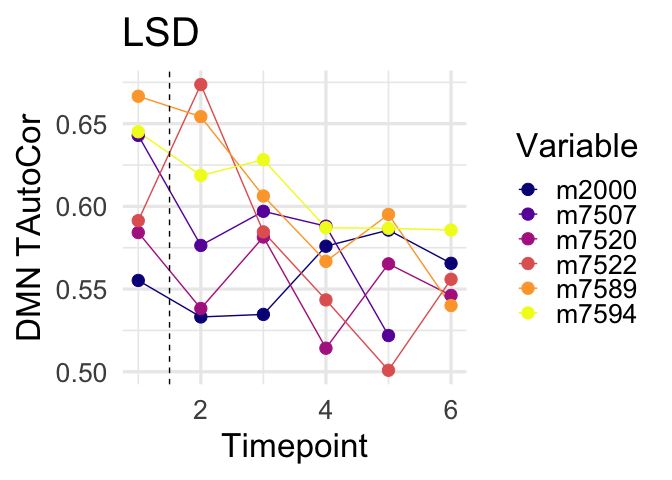
\includegraphics{Stats_n_Viz_files/figure-latex/unnamed-chunk-4-1.pdf}

\begin{Shaded}
\begin{Highlighting}[]
\CommentTok{\# generate extended color pal for subject plotting}
\FunctionTok{library}\NormalTok{(grDevices)}
\CommentTok{\# Define the extended custom palette function}
\NormalTok{extended\_palette }\OtherTok{\textless{}{-}} \FunctionTok{colorRampPalette}\NormalTok{(}\FunctionTok{rev}\NormalTok{(}\FunctionTok{c}\NormalTok{(}\StringTok{"\#FFEE00"}\NormalTok{, }\StringTok{"\#EF9500"}\NormalTok{, }\StringTok{"\#002642"}\NormalTok{, }\StringTok{"\#c1004f"}\NormalTok{, }\StringTok{"\#000000"}\NormalTok{)))}

\CommentTok{\# Generate a palette with the number of unique levels in V1}
\NormalTok{num\_colors }\OtherTok{\textless{}{-}} \FunctionTok{length}\NormalTok{(}\FunctionTok{unique}\NormalTok{(mergedDf\_clean}\SpecialCharTok{$}\NormalTok{Subjects))}
\NormalTok{generated\_colors }\OtherTok{\textless{}{-}} \FunctionTok{extended\_palette}\NormalTok{(num\_colors)}

\CommentTok{\# get head{-}motion regressed values for plotting}
\NormalTok{model\_to\_reg }\OtherTok{\textless{}{-}} \FunctionTok{lm}\NormalTok{(TDProp1 }\SpecialCharTok{\textasciitilde{}}\NormalTok{ MeanFD }\SpecialCharTok{+}\NormalTok{ RemTRs}\SpecialCharTok{+}\NormalTok{Task, }\AttributeTok{data =}\NormalTok{ mergedDf\_clean)}
\NormalTok{mergedDf\_clean}\SpecialCharTok{$}\NormalTok{Residuals}\OtherTok{\textless{}{-}}\FunctionTok{resid}\NormalTok{(model\_to\_reg)}\SpecialCharTok{+}\FunctionTok{mean}\NormalTok{(mergedDf\_clean}\SpecialCharTok{$}\NormalTok{TDProp1)}

\CommentTok{\# updated with manual Gaussian jitter}
\CommentTok{\# Add Gaussian jitter to x values (e.g., Drug factor levels)}
\FunctionTok{set.seed}\NormalTok{(}\DecValTok{2}\NormalTok{)}
\NormalTok{mergedDf\_clean}\SpecialCharTok{$}\NormalTok{JitteredDrug }\OtherTok{\textless{}{-}} \FunctionTok{as.numeric}\NormalTok{(mergedDf\_clean}\SpecialCharTok{$}\NormalTok{Drug) }\SpecialCharTok{+} \FunctionTok{rnorm}\NormalTok{(}\FunctionTok{nrow}\NormalTok{(mergedDf\_clean), }\AttributeTok{mean =} \DecValTok{0}\NormalTok{, }\AttributeTok{sd =} \FloatTok{0.1}\NormalTok{)}

\CommentTok{\# figure 2a}
\FunctionTok{ggplot}\NormalTok{(mergedDf\_clean, }\FunctionTok{aes}\NormalTok{(}\AttributeTok{x =}\NormalTok{ JitteredDrug, }\AttributeTok{y =}\NormalTok{ Residuals)) }\SpecialCharTok{+}
  \FunctionTok{geom\_point}\NormalTok{(}\AttributeTok{alpha =} \FloatTok{0.8}\NormalTok{, }\AttributeTok{size =} \DecValTok{4}\NormalTok{, }\FunctionTok{aes}\NormalTok{(}\AttributeTok{color =}\NormalTok{ People)) }\SpecialCharTok{+}  \CommentTok{\# Points with Gaussian jitter}
  \FunctionTok{geom\_boxplot}\NormalTok{(}\FunctionTok{aes}\NormalTok{(}\AttributeTok{group =}\NormalTok{ Drug), }\AttributeTok{alpha =} \FloatTok{0.2}\NormalTok{, }\AttributeTok{outlier.shape =} \ConstantTok{NA}\NormalTok{, }\AttributeTok{width =} \FloatTok{0.25}\NormalTok{) }\SpecialCharTok{+}  \CommentTok{\# Boxplot}
  \FunctionTok{labs}\NormalTok{(}\AttributeTok{title =} \StringTok{"MDMA vs. Placebo }\SpecialCharTok{\textbackslash{}n}\StringTok{"}\NormalTok{,}
       \AttributeTok{x =} \StringTok{""}\NormalTok{,}
       \AttributeTok{y =} \StringTok{"\% Bottom{-}up"}\NormalTok{) }\SpecialCharTok{+} 
  \FunctionTok{scale\_x\_continuous}\NormalTok{(}\AttributeTok{breaks =} \DecValTok{1}\SpecialCharTok{:}\DecValTok{2}\NormalTok{, }\AttributeTok{labels =} \FunctionTok{c}\NormalTok{(}\StringTok{\textquotesingle{}Placebo\textquotesingle{}}\NormalTok{, }\StringTok{\textquotesingle{}MDMA\textquotesingle{}}\NormalTok{)) }\SpecialCharTok{+}
  \FunctionTok{scale\_color\_manual}\NormalTok{(}\AttributeTok{values =}\NormalTok{ generated\_colors)}\SpecialCharTok{+}
  \FunctionTok{theme\_minimal}\NormalTok{(}\AttributeTok{base\_size=}\DecValTok{28}\NormalTok{)}
\end{Highlighting}
\end{Shaded}

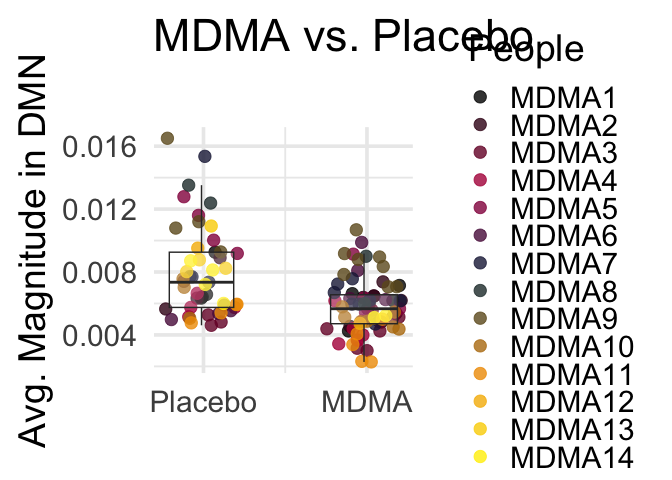
\includegraphics{Stats_n_Viz_files/figure-latex/unnamed-chunk-4-2.pdf}

\begin{Shaded}
\begin{Highlighting}[]
\CommentTok{\# job application version {-} 350 x 650}
\FunctionTok{ggplot}\NormalTok{(mergedDf\_clean, }\FunctionTok{aes}\NormalTok{(}\AttributeTok{x =}\NormalTok{ Drug, }\AttributeTok{y =}\NormalTok{ Residuals)) }\SpecialCharTok{+}
  \FunctionTok{geom\_jitter}\NormalTok{(}\AttributeTok{width =} \FloatTok{0.25}\NormalTok{, }\AttributeTok{height =} \DecValTok{0}\NormalTok{, }\AttributeTok{alpha =} \FloatTok{0.8}\NormalTok{, }\AttributeTok{size =} \DecValTok{2}\NormalTok{, }\FunctionTok{aes}\NormalTok{(}\AttributeTok{color =}\NormalTok{ People)) }\SpecialCharTok{+}  \CommentTok{\# Jittered points}
  \FunctionTok{geom\_boxplot}\NormalTok{(}\AttributeTok{alpha =} \FloatTok{0.2}\NormalTok{, }\AttributeTok{outlier.shape =} \ConstantTok{NA}\NormalTok{) }\SpecialCharTok{+}     \CommentTok{\# Boxplot}
  \FunctionTok{labs}\NormalTok{(}\AttributeTok{x =} \StringTok{""}\NormalTok{,}
       \AttributeTok{y =} \StringTok{"\% Bottom{-}up"}\NormalTok{) }\SpecialCharTok{+}
  \FunctionTok{scale\_x\_discrete}\NormalTok{(}\AttributeTok{labels =} \FunctionTok{c}\NormalTok{(}\StringTok{\textquotesingle{}Placebo\textquotesingle{}}\NormalTok{, }\StringTok{\textquotesingle{}MDMA\textquotesingle{}}\NormalTok{)) }\SpecialCharTok{+}
  \FunctionTok{scale\_color\_manual}\NormalTok{(}\AttributeTok{values =}\NormalTok{ generated\_colors) }\SpecialCharTok{+}  \CommentTok{\# Custom generated color palette}
  \FunctionTok{theme\_minimal}\NormalTok{(}\AttributeTok{base\_size =} \DecValTok{28}\NormalTok{)}\SpecialCharTok{+}
  \FunctionTok{theme}\NormalTok{(}\AttributeTok{legend.position =} \StringTok{"none"}\NormalTok{,}\AttributeTok{axis.text.x=}\FunctionTok{element\_text}\NormalTok{(}\AttributeTok{angle=}\DecValTok{45}\NormalTok{))}
\end{Highlighting}
\end{Shaded}

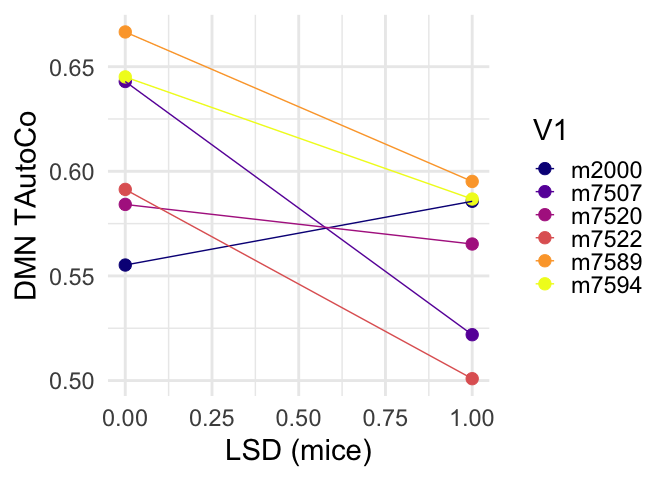
\includegraphics{Stats_n_Viz_files/figure-latex/unnamed-chunk-4-3.pdf}

\begin{Shaded}
\begin{Highlighting}[]
\CommentTok{\# full model for stats}
\NormalTok{fit\_lme }\OtherTok{\textless{}{-}} \FunctionTok{lme}\NormalTok{(TDProp1 }\SpecialCharTok{\textasciitilde{}}\NormalTok{ Drug }\SpecialCharTok{+}\NormalTok{ RemTRs }\SpecialCharTok{+}\NormalTok{ MeanFD}\SpecialCharTok{+}\NormalTok{Task, }\AttributeTok{random =} \SpecialCharTok{\textasciitilde{}} \DecValTok{1} \SpecialCharTok{|}\NormalTok{ Subjects, }\AttributeTok{data =}\NormalTok{ mergedDf\_clean)}
\NormalTok{summaryLME}\OtherTok{\textless{}{-}}\FunctionTok{summary}\NormalTok{(fit\_lme)}

\CommentTok{\# testing lme4 for robustness}
\FunctionTok{library}\NormalTok{(lme4)}
\end{Highlighting}
\end{Shaded}

\begin{verbatim}
## Loading required package: Matrix
\end{verbatim}

\begin{verbatim}
## 
## Attaching package: 'lme4'
\end{verbatim}

\begin{verbatim}
## The following object is masked from 'package:nlme':
## 
##     lmList
\end{verbatim}

\begin{Shaded}
\begin{Highlighting}[]
\FunctionTok{library}\NormalTok{(lmerTest)}
\end{Highlighting}
\end{Shaded}

\begin{verbatim}
## 
## Attaching package: 'lmerTest'
\end{verbatim}

\begin{verbatim}
## The following object is masked from 'package:lme4':
## 
##     lmer
\end{verbatim}

\begin{verbatim}
## The following object is masked from 'package:stats':
## 
##     step
\end{verbatim}

\begin{Shaded}
\begin{Highlighting}[]
\NormalTok{fit\_lmer }\OtherTok{\textless{}{-}} \FunctionTok{lmer}\NormalTok{(TDProp1 }\SpecialCharTok{\textasciitilde{}}\NormalTok{ Drug }\SpecialCharTok{+}\NormalTok{ RemTRs }\SpecialCharTok{+}\NormalTok{ MeanFD}\SpecialCharTok{+}\NormalTok{Task }\SpecialCharTok{+}\NormalTok{ (}\DecValTok{1} \SpecialCharTok{|}\NormalTok{ Subjects), }\AttributeTok{data =}\NormalTok{ mergedDf\_clean)}
\end{Highlighting}
\end{Shaded}

\begin{verbatim}
## Warning: Some predictor variables are on very different scales: consider
## rescaling
## Warning: Some predictor variables are on very different scales: consider
## rescaling
\end{verbatim}

\begin{Shaded}
\begin{Highlighting}[]
\CommentTok{\# checks out}

\DocumentationTok{\#\#\#\#\#}
\DocumentationTok{\#\#\#\# with all non{-}drug scans: Figure 2b}
\DocumentationTok{\#\#\#\#\#}

\CommentTok{\# get head{-}motion regressed values for plotting}
\NormalTok{model\_to\_reg }\OtherTok{\textless{}{-}} \FunctionTok{lm}\NormalTok{(TDProp1 }\SpecialCharTok{\textasciitilde{}}\NormalTok{ MeanFD }\SpecialCharTok{+}\NormalTok{ RemTRs}\SpecialCharTok{+}\NormalTok{Task, }\AttributeTok{data =}\NormalTok{ mergedDf)}
\NormalTok{mergedDf}\SpecialCharTok{$}\NormalTok{Residuals}\OtherTok{\textless{}{-}}\FunctionTok{resid}\NormalTok{(model\_to\_reg)}\SpecialCharTok{+}\FunctionTok{mean}\NormalTok{(mergedDf}\SpecialCharTok{$}\NormalTok{TDProp1)}

\CommentTok{\# updated with manual Gaussian jitter}
\CommentTok{\# Add Gaussian jitter to x values (e.g., Drug factor levels)}
\FunctionTok{set.seed}\NormalTok{(}\DecValTok{1}\NormalTok{)}
\NormalTok{mergedDf}\SpecialCharTok{$}\NormalTok{JitteredDrug }\OtherTok{\textless{}{-}} \FunctionTok{as.numeric}\NormalTok{(mergedDf}\SpecialCharTok{$}\NormalTok{Drug) }\SpecialCharTok{+} \FunctionTok{rnorm}\NormalTok{(}\FunctionTok{nrow}\NormalTok{(mergedDf), }\AttributeTok{mean =} \DecValTok{0}\NormalTok{, }\AttributeTok{sd =} \FloatTok{0.1}\NormalTok{)}

\CommentTok{\# figure 2a}
\FunctionTok{ggplot}\NormalTok{(mergedDf, }\FunctionTok{aes}\NormalTok{(}\AttributeTok{x =}\NormalTok{ JitteredDrug, }\AttributeTok{y =}\NormalTok{ Residuals)) }\SpecialCharTok{+}
  \FunctionTok{geom\_point}\NormalTok{(}\AttributeTok{alpha =} \FloatTok{0.8}\NormalTok{, }\AttributeTok{size =} \DecValTok{4}\NormalTok{, }\FunctionTok{aes}\NormalTok{(}\AttributeTok{color =}\NormalTok{ People)) }\SpecialCharTok{+}  \CommentTok{\# Points with Gaussian jitter}
  \FunctionTok{geom\_boxplot}\NormalTok{(}\FunctionTok{aes}\NormalTok{(}\AttributeTok{group =}\NormalTok{ Drug), }\AttributeTok{alpha =} \FloatTok{0.2}\NormalTok{, }\AttributeTok{outlier.shape =} \ConstantTok{NA}\NormalTok{, }\AttributeTok{width =} \FloatTok{0.25}\NormalTok{) }\SpecialCharTok{+}  \CommentTok{\# Boxplot}
  \FunctionTok{labs}\NormalTok{(}\AttributeTok{title =} \StringTok{"MDMA vs. No{-}drug scans }\SpecialCharTok{\textbackslash{}n}\StringTok{"}\NormalTok{,}
       \AttributeTok{x =} \StringTok{""}\NormalTok{,}
       \AttributeTok{y =} \StringTok{"\% Bottom{-}up"}\NormalTok{) }\SpecialCharTok{+} 
  \FunctionTok{scale\_x\_continuous}\NormalTok{(}\AttributeTok{breaks =} \DecValTok{1}\SpecialCharTok{:}\DecValTok{2}\NormalTok{, }\AttributeTok{labels =} \FunctionTok{c}\NormalTok{(}\StringTok{\textquotesingle{}No Drug\textquotesingle{}}\NormalTok{, }\StringTok{\textquotesingle{}MDMA\textquotesingle{}}\NormalTok{)) }\SpecialCharTok{+}
  \FunctionTok{theme\_minimal}\NormalTok{(}\AttributeTok{base\_size =} \DecValTok{25}\NormalTok{) }\SpecialCharTok{+}
  \FunctionTok{scale\_color\_manual}\NormalTok{(}\AttributeTok{values =}\NormalTok{ generated\_colors)}
\end{Highlighting}
\end{Shaded}

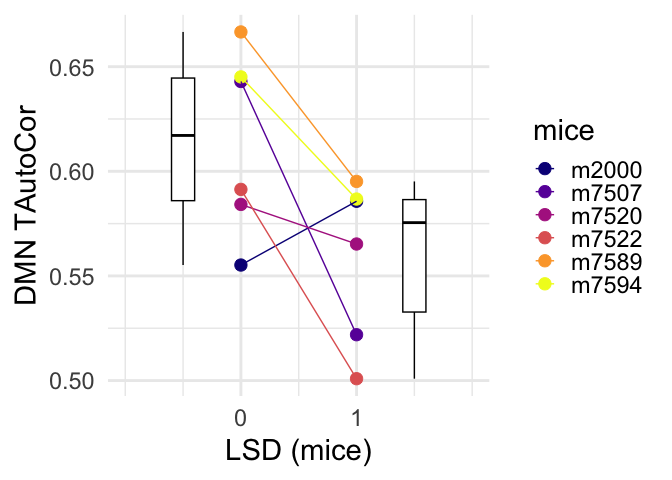
\includegraphics{Stats_n_Viz_files/figure-latex/unnamed-chunk-4-4.pdf}

\begin{Shaded}
\begin{Highlighting}[]
\CommentTok{\# figure 2a}
\CommentTok{\#ggplot(mergedDf, aes(x = Drug, y = Residuals)) +}
\CommentTok{\#  geom\_jitter(width = 0.25, height = 0, alpha = 0.8,size=4,aes(color = People)) +  \# Jittered points}
\CommentTok{\#  geom\_boxplot(alpha = 0.2,outlier.shape = NA) +     \# Boxplot}
\CommentTok{\#  labs(title = "MDMA vs. No{-}drug scans \textbackslash{}n",}
\CommentTok{\#       x = "",}
\CommentTok{\#       y = "\% Bottom{-}up") + scale\_x\_discrete(labels=c(\textquotesingle{}No Drug\textquotesingle{},\textquotesingle{}MDMA\textquotesingle{}))+}
\CommentTok{\#  theme\_minimal(base\_size=25)+scale\_color\_manual(values = generated\_colors)}

\CommentTok{\# full model for stats}
\NormalTok{fit\_lme }\OtherTok{\textless{}{-}} \FunctionTok{lme}\NormalTok{(TDProp1 }\SpecialCharTok{\textasciitilde{}}\NormalTok{ Drug }\SpecialCharTok{+}\NormalTok{ RemTRs }\SpecialCharTok{+}\NormalTok{ MeanFD}\SpecialCharTok{+}\NormalTok{Task, }\AttributeTok{random =} \SpecialCharTok{\textasciitilde{}} \DecValTok{1} \SpecialCharTok{|}\NormalTok{ Subjects, }\AttributeTok{data =}\NormalTok{ mergedDf)}
\NormalTok{summaryLME}\OtherTok{\textless{}{-}}\FunctionTok{summary}\NormalTok{(fit\_lme)}

\CommentTok{\# lme4 test for robustness}
\NormalTok{fit\_lmer }\OtherTok{\textless{}{-}} \FunctionTok{lmer}\NormalTok{(TDProp1 }\SpecialCharTok{\textasciitilde{}}\NormalTok{ Drug }\SpecialCharTok{+}\NormalTok{ RemTRs }\SpecialCharTok{+}\NormalTok{ MeanFD}\SpecialCharTok{+}\NormalTok{Task }\SpecialCharTok{+}\NormalTok{ (}\DecValTok{1} \SpecialCharTok{|}\NormalTok{ Subjects), }\AttributeTok{data =}\NormalTok{ mergedDf)}
\end{Highlighting}
\end{Shaded}

\begin{verbatim}
## Warning: Some predictor variables are on very different scales: consider
## rescaling
## Warning: Some predictor variables are on very different scales: consider
## rescaling
\end{verbatim}

\begin{Shaded}
\begin{Highlighting}[]
\CommentTok{\# checks out}

\CommentTok{\# make a "people"{-}"subjects" equivalence data frame to reference in figures down below}
\NormalTok{unique\_pairs }\OtherTok{\textless{}{-}} \FunctionTok{unique}\NormalTok{(mergedDf[}\FunctionTok{c}\NormalTok{(}\StringTok{"People"}\NormalTok{, }\StringTok{"Subjects"}\NormalTok{)])}
\end{Highlighting}
\end{Shaded}

\begin{Shaded}
\begin{Highlighting}[]
\CommentTok{\# extract standout sessions/participants}
\FunctionTok{library}\NormalTok{(dplyr)}
\end{Highlighting}
\end{Shaded}

\begin{verbatim}
## 
## Attaching package: 'dplyr'
\end{verbatim}

\begin{verbatim}
## The following object is masked from 'package:nlme':
## 
##     collapse
\end{verbatim}

\begin{verbatim}
## The following objects are masked from 'package:stats':
## 
##     filter, lag
\end{verbatim}

\begin{verbatim}
## The following objects are masked from 'package:base':
## 
##     intersect, setdiff, setequal, union
\end{verbatim}

\begin{Shaded}
\begin{Highlighting}[]
\CommentTok{\# Calculate the difference in TDProp1 between Drug and Placebo conditions}
\NormalTok{df\_diff }\OtherTok{\textless{}{-}}\NormalTok{ mergedDf\_clean }\SpecialCharTok{\%\textgreater{}\%}
  \FunctionTok{group\_by}\NormalTok{(Subjects) }\SpecialCharTok{\%\textgreater{}\%}
  \FunctionTok{summarise}\NormalTok{(}\AttributeTok{Diff\_TDProp1 =} \FunctionTok{mean}\NormalTok{(TDProp1[Drug }\SpecialCharTok{==} \DecValTok{0}\NormalTok{]}\SpecialCharTok{{-}}\FunctionTok{mean}\NormalTok{(TDProp1[Drug }\SpecialCharTok{==} \DecValTok{1}\NormalTok{]), }\AttributeTok{na.rm =} \ConstantTok{TRUE}\NormalTok{))}

\CommentTok{\# Identify the participant with the greatest increase in TDProp1}
\NormalTok{max\_diff\_subject }\OtherTok{\textless{}{-}}\NormalTok{ df\_diff }\SpecialCharTok{\%\textgreater{}\%}
  \FunctionTok{filter}\NormalTok{(Diff\_TDProp1 }\SpecialCharTok{==} \FunctionTok{max}\NormalTok{(Diff\_TDProp1, }\AttributeTok{na.rm =} \ConstantTok{TRUE}\NormalTok{)) }\SpecialCharTok{\%\textgreater{}\%}
  \FunctionTok{pull}\NormalTok{(Subjects)}

\FunctionTok{print}\NormalTok{(max\_diff\_subject)}
\end{Highlighting}
\end{Shaded}

\begin{verbatim}
## [1] sub-MDMA017
## 14 Levels: sub-MDMA001 sub-MDMA002 sub-MDMA003 sub-MDMA005 ... sub-MDMA017
\end{verbatim}

\begin{Shaded}
\begin{Highlighting}[]
\CommentTok{\# added chunk to code which sessions are post{-}mdma in macro timeline of study}

\CommentTok{\# initialize new column in mergedDf}
\NormalTok{mergedDf}\SpecialCharTok{$}\NormalTok{PostMDMASession }\OtherTok{\textless{}{-}} \DecValTok{2}

\CommentTok{\# load in subjSeshDoseCorrep (read delim, sep=\textquotesingle{} \textquotesingle{})}
\NormalTok{subjSeshDoseCorrep }\OtherTok{\textless{}{-}} \FunctionTok{read.table}\NormalTok{(}\StringTok{"\textasciitilde{}/Downloads/subjSeshDoseCorresp.csv"}\NormalTok{, }\AttributeTok{sep =} \StringTok{\textquotesingle{} \textquotesingle{}}\NormalTok{)}

\CommentTok{\# for each subject}
\ControlFlowTok{for}\NormalTok{ (i }\ControlFlowTok{in} \DecValTok{1}\SpecialCharTok{:}\FunctionTok{nrow}\NormalTok{(subjSeshDoseCorrep)) \{}
  \CommentTok{\# if i \textless{}10}
  \ControlFlowTok{if}\NormalTok{(i}\SpecialCharTok{\textless{}}\DecValTok{10}\NormalTok{)\{}
\NormalTok{    subjectID }\OtherTok{\textless{}{-}} \FunctionTok{paste0}\NormalTok{(}\StringTok{"sub{-}MDMA00"}\NormalTok{, i)  }\CommentTok{\# Reconstruct subject ID}
\NormalTok{  \} }\ControlFlowTok{else} \ControlFlowTok{if}\NormalTok{(i}\SpecialCharTok{\textgreater{}}\DecValTok{9}\NormalTok{)\{}
\NormalTok{    subjectID }\OtherTok{\textless{}{-}} \FunctionTok{paste0}\NormalTok{(}\StringTok{"sub{-}MDMA0"}\NormalTok{, i)  }\CommentTok{\# Reconstruct subject ID}
\NormalTok{  \}}
  \CommentTok{\# get position of placebo}
\NormalTok{  placeboPos }\OtherTok{\textless{}{-}} \FunctionTok{which}\NormalTok{(subjSeshDoseCorrep[i, }\DecValTok{2}\SpecialCharTok{:}\DecValTok{5}\NormalTok{] }\SpecialCharTok{==} \StringTok{"ses{-}01"}\NormalTok{)}
  \FunctionTok{print}\NormalTok{(placeboPos)}
  \CommentTok{\# get position in mergedDf}
\NormalTok{  placeboRows }\OtherTok{\textless{}{-}}\NormalTok{ mergedDf}\SpecialCharTok{$}\NormalTok{Subject }\SpecialCharTok{==}\NormalTok{ subjectID }\SpecialCharTok{\&}\NormalTok{ mergedDf}\SpecialCharTok{$}\NormalTok{Dosage }\SpecialCharTok{==} \StringTok{"Placebo"}
  \CommentTok{\# baseline is pos one, placebo is pos 2, 80 is pos 3, 120 is pos 4}
  \CommentTok{\# if placebo is ses{-}01, leave as initialize 0}
  \CommentTok{\# if placebo is ses{-}02, 1 for post{-}drugMacro}
  \CommentTok{\# if placebo is ses{-}03, 1 for post{-}drugMacro}
  \ControlFlowTok{if}\NormalTok{ (placeboPos }\SpecialCharTok{==} \DecValTok{2}\NormalTok{) \{}
\NormalTok{      mergedDf}\SpecialCharTok{$}\NormalTok{PostMDMASession[placeboRows] }\OtherTok{\textless{}{-}} \DecValTok{0}
\NormalTok{    \} }\ControlFlowTok{else} \ControlFlowTok{if}\NormalTok{ (placeboPos }\SpecialCharTok{==} \DecValTok{3}\NormalTok{ ) \{}
\NormalTok{      mergedDf}\SpecialCharTok{$}\NormalTok{PostMDMASession[placeboRows] }\OtherTok{\textless{}{-}} \DecValTok{1}
\NormalTok{    \} }\ControlFlowTok{else} \ControlFlowTok{if}\NormalTok{ (placeboPos }\SpecialCharTok{==} \DecValTok{4}\NormalTok{) \{}
\NormalTok{      mergedDf}\SpecialCharTok{$}\NormalTok{PostMDMASession[placeboRows] }\OtherTok{\textless{}{-}} \DecValTok{1}
\NormalTok{    \}}
\NormalTok{\}}
\end{Highlighting}
\end{Shaded}

\begin{verbatim}
## [1] 3
## [1] 2
## [1] 3
## [1] 2
## [1] 4
## [1] 3
## [1] 3
## [1] 2
## [1] 2
## [1] 4
## [1] 2
## [1] 3
## [1] 4
## [1] 4
## [1] 2
## [1] 3
## [1] 2
\end{verbatim}

\begin{Shaded}
\begin{Highlighting}[]
\CommentTok{\# make post drug a separate placebo condition}
\NormalTok{mergedDf}\SpecialCharTok{$}\NormalTok{Drug2}\OtherTok{\textless{}{-}}\FunctionTok{as.numeric}\NormalTok{(mergedDf}\SpecialCharTok{$}\NormalTok{Drug)}
\NormalTok{mergedDf}\SpecialCharTok{$}\NormalTok{Drug2[mergedDf}\SpecialCharTok{$}\NormalTok{PostMDMASession}\SpecialCharTok{==}\DecValTok{1}\NormalTok{]}\OtherTok{=}\DecValTok{3}
\CommentTok{\# placebo pre{-}drug is 1}
\CommentTok{\# placebo post{-}drug is 3}
\CommentTok{\# drug is 2}

\NormalTok{mergedDf}\SpecialCharTok{$}\NormalTok{Drug2}\OtherTok{\textless{}{-}}\FunctionTok{as.factor}\NormalTok{(mergedDf}\SpecialCharTok{$}\NormalTok{Drug2)}
\NormalTok{mergedDf }\OtherTok{\textless{}{-}} \FunctionTok{within}\NormalTok{(mergedDf, Drug2 }\OtherTok{\textless{}{-}} \FunctionTok{relevel}\NormalTok{(Drug2, }\AttributeTok{ref =} \DecValTok{1}\NormalTok{))}
\CommentTok{\# set MDMA visits to post MDMA}
\NormalTok{mergedDf}\SpecialCharTok{$}\NormalTok{PostMDMASession[mergedDf}\SpecialCharTok{$}\NormalTok{Drug}\SpecialCharTok{==}\DecValTok{1}\NormalTok{]}\OtherTok{=}\DecValTok{1}

\NormalTok{model }\OtherTok{\textless{}{-}} \FunctionTok{lme}\NormalTok{(TDProp1 }\SpecialCharTok{\textasciitilde{}}\NormalTok{ MeanFD }\SpecialCharTok{+}\NormalTok{Drug2}\SpecialCharTok{+}\NormalTok{ RemTRs, }\AttributeTok{random =} \SpecialCharTok{\textasciitilde{}} \DecValTok{1} \SpecialCharTok{|}\NormalTok{ Subjects, }\AttributeTok{data =}\NormalTok{ mergedDf)}
\end{Highlighting}
\end{Shaded}

\begin{Shaded}
\begin{Highlighting}[]
\CommentTok{\#meltedDf \textless{}{-} melt(mergedDf, id.vars = c("Subjects", "Task", "Dosage", "Session", "SpikesPercent", "MeanFD", "RemTRs", "Drug"))}
\CommentTok{\#meltedDf \textless{}{-} within(meltedDf, variable \textless{}{-} relevel(variable, ref = 3))}
\CommentTok{\#model \textless{}{-} lme(value \textasciitilde{} MeanFD + Drug + RemTRs+variable+variable*Drug+MeanFD*variable+RemTRs*variable, random = \textasciitilde{} 1 | Subjects/variable, data = meltedDf)}
\CommentTok{\#summary(model)}
\CommentTok{\#sjPlot::plot\_model(model, type = "eff",show.values = T)}
\CommentTok{\#}
\DocumentationTok{\#\# great, now let\textquotesingle{}s bootstrap it}
\DocumentationTok{\#\# Set the number of bootstrap samples}
\CommentTok{\#num\_bootstrap\_samples \textless{}{-} }
\DocumentationTok{\#\# initialize t vectors}
\CommentTok{\#td1\_d\textless{}{-}zeros(num\_bootstrap\_samples,1)}
\CommentTok{\#td1\_fd\textless{}{-}zeros(num\_bootstrap\_samples,1)}
\CommentTok{\#td2\_d\textless{}{-}zeros(num\_bootstrap\_samples,1)}
\CommentTok{\#td2\_fd\textless{}{-}zeros(num\_bootstrap\_samples,1)}
\CommentTok{\#td3\_d\textless{}{-}zeros(num\_bootstrap\_samples,1)}
\CommentTok{\#td3\_fd\textless{}{-}zeros(num\_bootstrap\_samples,1)}
\CommentTok{\#td4\_d\textless{}{-}zeros(num\_bootstrap\_samples,1)}
\CommentTok{\#td4\_fd\textless{}{-}zeros(num\_bootstrap\_samples,1)}
\CommentTok{\#}
\DocumentationTok{\#\# bootstrap loops}
\CommentTok{\#set.seed(420)}
\CommentTok{\#for (i in 1:num\_bootstrap\_samples)\{}
\CommentTok{\#  \# resample subjects instead of observations to be conserative}
\CommentTok{\#   BootSubjs=sample(unique(mergedDf$Subjects),14,replace=T)}
\CommentTok{\#   \# Create an empty dataframe to store the resampled observations}
\CommentTok{\#   bootSamp \textless{}{-} data.frame()}
\CommentTok{\#   for (j in 1:length(BootSubjs))\{}
\CommentTok{\#       subject\_obs \textless{}{-} meltedDf[meltedDf$Subjects == BootSubjs[j], ]}
\CommentTok{\#       bootSamp \textless{}{-} rbind(bootSamp, subject\_obs)}
\CommentTok{\#   \}}
\CommentTok{\#  \# fit model}
\CommentTok{\#  model\_i \textless{}{-} lme(value \textasciitilde{} MeanFD + Drug + RemTRs+variable+variable*Drug+variable*MeanFD, random = \textasciitilde{} 1 | Subjects/variable, data = bootSamp)}
\CommentTok{\#  \# get t{-}values}
\CommentTok{\#  td1\_d[i]=summary(model\_i)$tTable[rownames(summary(model\_i)$tTable) == "Drug1:variableTDProp1", "t{-}value"]}
\CommentTok{\#  td1\_fd[i]=summary(model\_i)$tTable[rownames(summary(model\_i)$tTable) == "MeanFD:variableTDProp1", "t{-}value"]}
\CommentTok{\#  td3\_d[i]=summary(model\_i)$tTable[rownames(summary(model\_i)$tTable) == "Drug1:variableTDProp3", "t{-}value"]}
\CommentTok{\#  td3\_fd[i]=summary(model\_i)$tTable[rownames(summary(model\_i)$tTable) == "MeanFD:variableTDProp3", "t{-}value"]}
\CommentTok{\#  td4\_d[i]=summary(model\_i)$tTable[rownames(summary(model\_i)$tTable) == "Drug1:variableTDProp4", "t{-}value"]}
\CommentTok{\#  td4\_fd[i]=summary(model\_i)$tTable[rownames(summary(model\_i)$tTable) == "MeanFD:variableTDProp4", "t{-}value"]}
\CommentTok{\#\}}
\CommentTok{\#}
\CommentTok{\#bootstrap\_results=data.frame(cbind(td1\_d,td1\_fd,td3\_d,td3\_fd,td4\_d,td4\_fd))}
\CommentTok{\#colnames(bootstrap\_results)=c(\textquotesingle{}td1\_drug\textquotesingle{},\textquotesingle{}td1\_fd\textquotesingle{},\textquotesingle{}td3\_drug\textquotesingle{},\textquotesingle{}td3\_fd\textquotesingle{},\textquotesingle{}td4\_drug\textquotesingle{},\textquotesingle{}td4\_fd\textquotesingle{})}
\CommentTok{\#plotdf=melt(bootstrap\_results)}
\CommentTok{\#}
\DocumentationTok{\#\# Create box{-}and{-}whisker plots}
\CommentTok{\#ggplot(plotdf, aes(x = variable, y = value,)) +}
\CommentTok{\#  geom\_boxplot(position = position\_dodge(width = 0.8)) +}
\CommentTok{\#  labs(x = "Model", y = "T{-}Values", title = "Bootstrap T{-}Values for Drug and MeanFD") +}
\CommentTok{\#  theme\_minimal(base\_size = 16)+scale\_fill\_manual(values=c(\textquotesingle{}blue\textquotesingle{},\textquotesingle{}red\textquotesingle{}))}
\end{Highlighting}
\end{Shaded}

\begin{Shaded}
\begin{Highlighting}[]
\CommentTok{\# autocorrelation}
\NormalTok{rs1}\OtherTok{=}\FunctionTok{read.csv}\NormalTok{(}\StringTok{\textquotesingle{}\textasciitilde{}/Downloads/rs1\_TAutoCorMerged.csv\textquotesingle{}}\NormalTok{,}\AttributeTok{header=}\NormalTok{F)}
\NormalTok{rs2}\OtherTok{=}\FunctionTok{read.csv}\NormalTok{(}\StringTok{\textquotesingle{}\textasciitilde{}/Downloads/rs2\_TAutoCorMerged.csv\textquotesingle{}}\NormalTok{,}\AttributeTok{header=}\NormalTok{F)}
\NormalTok{emo}\OtherTok{=}\FunctionTok{read.csv}\NormalTok{(}\StringTok{\textquotesingle{}\textasciitilde{}/Downloads/emotion\_TAutoCorMerged.csv\textquotesingle{}}\NormalTok{,}\AttributeTok{header=}\NormalTok{F)}
\NormalTok{gambling}\OtherTok{=}\FunctionTok{read.csv}\NormalTok{(}\StringTok{\textquotesingle{}\textasciitilde{}/Downloads/gambling\_TAutoCorMerged.csv\textquotesingle{}}\NormalTok{,}\AttributeTok{header=}\NormalTok{F)}
\NormalTok{wm}\OtherTok{=}\FunctionTok{read.csv}\NormalTok{(}\StringTok{\textquotesingle{}\textasciitilde{}/Downloads/wm\_TAutoCorMerged.csv\textquotesingle{}}\NormalTok{,}\AttributeTok{header=}\NormalTok{F)}
\CommentTok{\# set colnames}
\CommentTok{\#colnames(rs1)=c(\textquotesingle{}bvProp\textquotesingle{},\textquotesingle{}pProp\textquotesingle{},\textquotesingle{}m1Prop\textquotesingle{},\textquotesingle{}m2Prop\textquotesingle{},\textquotesingle{}bvTRs\textquotesingle{},\textquotesingle{}pTRs\textquotesingle{},\textquotesingle{}m1TRs\textquotesingle{},\textquotesingle{}m2TRs\textquotesingle{})}
\CommentTok{\#colnames(rs2)=c(\textquotesingle{}bvProp\textquotesingle{},\textquotesingle{}pProp\textquotesingle{},\textquotesingle{}m1Prop\textquotesingle{},\textquotesingle{}m2Prop\textquotesingle{},\textquotesingle{}bvTRs\textquotesingle{},\textquotesingle{}pTRs\textquotesingle{},\textquotesingle{}m1TRs\textquotesingle{},\textquotesingle{}m2TRs\textquotesingle{})}
\CommentTok{\#colnames(emo)=c(\textquotesingle{}bvProp\textquotesingle{},\textquotesingle{}pProp\textquotesingle{},\textquotesingle{}m1Prop\textquotesingle{},\textquotesingle{}m2Prop\textquotesingle{},\textquotesingle{}bvTRs\textquotesingle{},\textquotesingle{}pTRs\textquotesingle{},\textquotesingle{}m1TRs\textquotesingle{},\textquotesingle{}m2TRs\textquotesingle{})}
\CommentTok{\#colnames(gambling)=c(\textquotesingle{}bvProp\textquotesingle{},\textquotesingle{}pProp\textquotesingle{},\textquotesingle{}m1Prop\textquotesingle{},\textquotesingle{}m2Prop\textquotesingle{},\textquotesingle{}bvTRs\textquotesingle{},\textquotesingle{}pTRs\textquotesingle{},\textquotesingle{}m1TRs\textquotesingle{},\textquotesingle{}m2TRs\textquotesingle{})}
\CommentTok{\#colnames(wm)=c(\textquotesingle{}bvProp\textquotesingle{},\textquotesingle{}pProp\textquotesingle{},\textquotesingle{}m1Prop\textquotesingle{},\textquotesingle{}m2Prop\textquotesingle{},\textquotesingle{}bvTRs\textquotesingle{},\textquotesingle{}pTRs\textquotesingle{},\textquotesingle{}m1TRs\textquotesingle{},\textquotesingle{}m2TRs\textquotesingle{})}
\NormalTok{rs1}\SpecialCharTok{$}\NormalTok{Task}\OtherTok{=}\StringTok{\textquotesingle{}rs\textquotesingle{}}
\NormalTok{rs2}\SpecialCharTok{$}\NormalTok{Task}\OtherTok{=}\StringTok{\textquotesingle{}rs2\textquotesingle{}}
\NormalTok{emo}\SpecialCharTok{$}\NormalTok{Task}\OtherTok{=}\StringTok{\textquotesingle{}emotion\textquotesingle{}}
\NormalTok{gambling}\SpecialCharTok{$}\NormalTok{Task}\OtherTok{=}\StringTok{\textquotesingle{}gambling\textquotesingle{}}
\NormalTok{wm}\SpecialCharTok{$}\NormalTok{Task}\OtherTok{=}\StringTok{\textquotesingle{}wm\textquotesingle{}}

\CommentTok{\# remove subj 4}
\NormalTok{rs1}\OtherTok{=}\NormalTok{rs1[}\SpecialCharTok{{-}}\FunctionTok{c}\NormalTok{(}\DecValTok{4}\NormalTok{),]}
\NormalTok{rs2}\OtherTok{=}\NormalTok{rs2[}\SpecialCharTok{{-}}\FunctionTok{c}\NormalTok{(}\DecValTok{4}\NormalTok{),]}
\NormalTok{emo}\OtherTok{=}\NormalTok{emo[}\SpecialCharTok{{-}}\FunctionTok{c}\NormalTok{(}\DecValTok{4}\NormalTok{),]}
\NormalTok{gambling}\OtherTok{=}\NormalTok{gambling[}\SpecialCharTok{{-}}\FunctionTok{c}\NormalTok{(}\DecValTok{4}\NormalTok{),]}
\NormalTok{wm}\OtherTok{=}\NormalTok{wm[}\SpecialCharTok{{-}}\FunctionTok{c}\NormalTok{(}\DecValTok{4}\NormalTok{),]}

\CommentTok{\# this is going to be ugly but simple}
\CommentTok{\# manually pair columns as sep. observations of baseline, placebo, 80, 120mg}
\NormalTok{rs1bv}\OtherTok{=}\FunctionTok{data.frame}\NormalTok{(}\FunctionTok{cbind}\NormalTok{(rs1}\SpecialCharTok{$}\NormalTok{V1,rs1}\SpecialCharTok{$}\NormalTok{V5))}
\NormalTok{rs1p}\OtherTok{=}\FunctionTok{data.frame}\NormalTok{(}\FunctionTok{cbind}\NormalTok{(rs1}\SpecialCharTok{$}\NormalTok{V2,rs1}\SpecialCharTok{$}\NormalTok{V6))}
\NormalTok{rs1m1}\OtherTok{=}\FunctionTok{data.frame}\NormalTok{(}\FunctionTok{cbind}\NormalTok{(rs1}\SpecialCharTok{$}\NormalTok{V3,rs1}\SpecialCharTok{$}\NormalTok{V7))}
\NormalTok{rs1m2}\OtherTok{=}\FunctionTok{data.frame}\NormalTok{(}\FunctionTok{cbind}\NormalTok{(rs1}\SpecialCharTok{$}\NormalTok{V4,rs1}\SpecialCharTok{$}\NormalTok{V8))}
\FunctionTok{colnames}\NormalTok{(rs1bv)}\OtherTok{=}\FunctionTok{c}\NormalTok{(}\StringTok{\textquotesingle{}AutoCor\textquotesingle{}}\NormalTok{,}\StringTok{\textquotesingle{}RemTRs\textquotesingle{}}\NormalTok{)}
\FunctionTok{colnames}\NormalTok{(rs1p)}\OtherTok{=}\FunctionTok{c}\NormalTok{(}\StringTok{\textquotesingle{}AutoCor\textquotesingle{}}\NormalTok{,}\StringTok{\textquotesingle{}RemTRs\textquotesingle{}}\NormalTok{)}
\FunctionTok{colnames}\NormalTok{(rs1m1)}\OtherTok{=}\FunctionTok{c}\NormalTok{(}\StringTok{\textquotesingle{}AutoCor\textquotesingle{}}\NormalTok{,}\StringTok{\textquotesingle{}RemTRs\textquotesingle{}}\NormalTok{)}
\FunctionTok{colnames}\NormalTok{(rs1m2)}\OtherTok{=}\FunctionTok{c}\NormalTok{(}\StringTok{\textquotesingle{}AutoCor\textquotesingle{}}\NormalTok{,}\StringTok{\textquotesingle{}RemTRs\textquotesingle{}}\NormalTok{)}

\NormalTok{rs2bv}\OtherTok{=}\FunctionTok{data.frame}\NormalTok{(}\FunctionTok{cbind}\NormalTok{(rs2}\SpecialCharTok{$}\NormalTok{V1,rs2}\SpecialCharTok{$}\NormalTok{V5))}
\NormalTok{rs2p}\OtherTok{=}\FunctionTok{data.frame}\NormalTok{(}\FunctionTok{cbind}\NormalTok{(rs2}\SpecialCharTok{$}\NormalTok{V2,rs2}\SpecialCharTok{$}\NormalTok{V6))}
\NormalTok{rs2m1}\OtherTok{=}\FunctionTok{data.frame}\NormalTok{(}\FunctionTok{cbind}\NormalTok{(rs2}\SpecialCharTok{$}\NormalTok{V3,rs2}\SpecialCharTok{$}\NormalTok{V7))}
\NormalTok{rs2m2}\OtherTok{=}\FunctionTok{data.frame}\NormalTok{(}\FunctionTok{cbind}\NormalTok{(rs2}\SpecialCharTok{$}\NormalTok{V4,rs2}\SpecialCharTok{$}\NormalTok{V8))}
\FunctionTok{colnames}\NormalTok{(rs2bv)}\OtherTok{=}\FunctionTok{c}\NormalTok{(}\StringTok{\textquotesingle{}AutoCor\textquotesingle{}}\NormalTok{,}\StringTok{\textquotesingle{}RemTRs\textquotesingle{}}\NormalTok{)}
\FunctionTok{colnames}\NormalTok{(rs2p)}\OtherTok{=}\FunctionTok{c}\NormalTok{(}\StringTok{\textquotesingle{}AutoCor\textquotesingle{}}\NormalTok{,}\StringTok{\textquotesingle{}RemTRs\textquotesingle{}}\NormalTok{)}
\FunctionTok{colnames}\NormalTok{(rs2m1)}\OtherTok{=}\FunctionTok{c}\NormalTok{(}\StringTok{\textquotesingle{}AutoCor\textquotesingle{}}\NormalTok{,}\StringTok{\textquotesingle{}RemTRs\textquotesingle{}}\NormalTok{)}
\FunctionTok{colnames}\NormalTok{(rs2m2)}\OtherTok{=}\FunctionTok{c}\NormalTok{(}\StringTok{\textquotesingle{}AutoCor\textquotesingle{}}\NormalTok{,}\StringTok{\textquotesingle{}RemTRs\textquotesingle{}}\NormalTok{)}

\NormalTok{emobv}\OtherTok{=}\FunctionTok{data.frame}\NormalTok{(}\FunctionTok{cbind}\NormalTok{(emo}\SpecialCharTok{$}\NormalTok{V1,emo}\SpecialCharTok{$}\NormalTok{V5))}
\NormalTok{emop}\OtherTok{=}\FunctionTok{data.frame}\NormalTok{(}\FunctionTok{cbind}\NormalTok{(emo}\SpecialCharTok{$}\NormalTok{V2,emo}\SpecialCharTok{$}\NormalTok{V6))}
\NormalTok{emom1}\OtherTok{=}\FunctionTok{data.frame}\NormalTok{(}\FunctionTok{cbind}\NormalTok{(emo}\SpecialCharTok{$}\NormalTok{V3,emo}\SpecialCharTok{$}\NormalTok{V7))}
\NormalTok{emom2}\OtherTok{=}\FunctionTok{data.frame}\NormalTok{(}\FunctionTok{cbind}\NormalTok{(emo}\SpecialCharTok{$}\NormalTok{V4,emo}\SpecialCharTok{$}\NormalTok{V8))}
\FunctionTok{colnames}\NormalTok{(emobv)}\OtherTok{=}\FunctionTok{c}\NormalTok{(}\StringTok{\textquotesingle{}AutoCor\textquotesingle{}}\NormalTok{,}\StringTok{\textquotesingle{}RemTRs\textquotesingle{}}\NormalTok{)}
\FunctionTok{colnames}\NormalTok{(emop)}\OtherTok{=}\FunctionTok{c}\NormalTok{(}\StringTok{\textquotesingle{}AutoCor\textquotesingle{}}\NormalTok{,}\StringTok{\textquotesingle{}RemTRs\textquotesingle{}}\NormalTok{)}
\FunctionTok{colnames}\NormalTok{(emom1)}\OtherTok{=}\FunctionTok{c}\NormalTok{(}\StringTok{\textquotesingle{}AutoCor\textquotesingle{}}\NormalTok{,}\StringTok{\textquotesingle{}RemTRs\textquotesingle{}}\NormalTok{)}
\FunctionTok{colnames}\NormalTok{(emom2)}\OtherTok{=}\FunctionTok{c}\NormalTok{(}\StringTok{\textquotesingle{}AutoCor\textquotesingle{}}\NormalTok{,}\StringTok{\textquotesingle{}RemTRs\textquotesingle{}}\NormalTok{)}

\NormalTok{gamblingbv}\OtherTok{=}\FunctionTok{data.frame}\NormalTok{(}\FunctionTok{cbind}\NormalTok{(gambling}\SpecialCharTok{$}\NormalTok{V1,gambling}\SpecialCharTok{$}\NormalTok{V5))}
\NormalTok{gamblingp}\OtherTok{=}\FunctionTok{data.frame}\NormalTok{(}\FunctionTok{cbind}\NormalTok{(gambling}\SpecialCharTok{$}\NormalTok{V2,gambling}\SpecialCharTok{$}\NormalTok{V6))}
\NormalTok{gamblingm1}\OtherTok{=}\FunctionTok{data.frame}\NormalTok{(}\FunctionTok{cbind}\NormalTok{(gambling}\SpecialCharTok{$}\NormalTok{V3,gambling}\SpecialCharTok{$}\NormalTok{V7))}
\NormalTok{gamblingm2}\OtherTok{=}\FunctionTok{data.frame}\NormalTok{(}\FunctionTok{cbind}\NormalTok{(gambling}\SpecialCharTok{$}\NormalTok{V4,gambling}\SpecialCharTok{$}\NormalTok{V8))}
\FunctionTok{colnames}\NormalTok{(gamblingbv)}\OtherTok{=}\FunctionTok{c}\NormalTok{(}\StringTok{\textquotesingle{}AutoCor\textquotesingle{}}\NormalTok{,}\StringTok{\textquotesingle{}RemTRs\textquotesingle{}}\NormalTok{)}
\FunctionTok{colnames}\NormalTok{(gamblingp)}\OtherTok{=}\FunctionTok{c}\NormalTok{(}\StringTok{\textquotesingle{}AutoCor\textquotesingle{}}\NormalTok{,}\StringTok{\textquotesingle{}RemTRs\textquotesingle{}}\NormalTok{)}
\FunctionTok{colnames}\NormalTok{(gamblingm1)}\OtherTok{=}\FunctionTok{c}\NormalTok{(}\StringTok{\textquotesingle{}AutoCor\textquotesingle{}}\NormalTok{,}\StringTok{\textquotesingle{}RemTRs\textquotesingle{}}\NormalTok{)}
\FunctionTok{colnames}\NormalTok{(gamblingm2)}\OtherTok{=}\FunctionTok{c}\NormalTok{(}\StringTok{\textquotesingle{}AutoCor\textquotesingle{}}\NormalTok{,}\StringTok{\textquotesingle{}RemTRs\textquotesingle{}}\NormalTok{)}

\NormalTok{wmbv}\OtherTok{=}\FunctionTok{data.frame}\NormalTok{(}\FunctionTok{cbind}\NormalTok{(wm}\SpecialCharTok{$}\NormalTok{V1,wm}\SpecialCharTok{$}\NormalTok{V5))}
\NormalTok{wmp}\OtherTok{=}\FunctionTok{data.frame}\NormalTok{(}\FunctionTok{cbind}\NormalTok{(wm}\SpecialCharTok{$}\NormalTok{V2,wm}\SpecialCharTok{$}\NormalTok{V6))}
\NormalTok{wmm1}\OtherTok{=}\FunctionTok{data.frame}\NormalTok{(}\FunctionTok{cbind}\NormalTok{(wm}\SpecialCharTok{$}\NormalTok{V3,wm}\SpecialCharTok{$}\NormalTok{V7))}
\NormalTok{wmm2}\OtherTok{=}\FunctionTok{data.frame}\NormalTok{(}\FunctionTok{cbind}\NormalTok{(wm}\SpecialCharTok{$}\NormalTok{V4,wm}\SpecialCharTok{$}\NormalTok{V8))}
\FunctionTok{colnames}\NormalTok{(wmbv)}\OtherTok{=}\FunctionTok{c}\NormalTok{(}\StringTok{\textquotesingle{}AutoCor\textquotesingle{}}\NormalTok{,}\StringTok{\textquotesingle{}RemTRs\textquotesingle{}}\NormalTok{)}
\FunctionTok{colnames}\NormalTok{(wmp)}\OtherTok{=}\FunctionTok{c}\NormalTok{(}\StringTok{\textquotesingle{}AutoCor\textquotesingle{}}\NormalTok{,}\StringTok{\textquotesingle{}RemTRs\textquotesingle{}}\NormalTok{)}
\FunctionTok{colnames}\NormalTok{(wmm1)}\OtherTok{=}\FunctionTok{c}\NormalTok{(}\StringTok{\textquotesingle{}AutoCor\textquotesingle{}}\NormalTok{,}\StringTok{\textquotesingle{}RemTRs\textquotesingle{}}\NormalTok{)}
\FunctionTok{colnames}\NormalTok{(wmm2)}\OtherTok{=}\FunctionTok{c}\NormalTok{(}\StringTok{\textquotesingle{}AutoCor\textquotesingle{}}\NormalTok{,}\StringTok{\textquotesingle{}RemTRs\textquotesingle{}}\NormalTok{)}

\CommentTok{\# get subject IDs from this rds}
\NormalTok{alff}\OtherTok{=}\FunctionTok{readRDS}\NormalTok{(}\StringTok{\textquotesingle{}\textasciitilde{}/OutPlacDrug\_alff.rds\textquotesingle{}}\NormalTok{)}
\NormalTok{rs1bv}\SpecialCharTok{$}\NormalTok{Subjects}\OtherTok{=}\NormalTok{alff}\SpecialCharTok{$}\NormalTok{SubjID}
\NormalTok{rs1p}\SpecialCharTok{$}\NormalTok{Subjects}\OtherTok{=}\NormalTok{alff}\SpecialCharTok{$}\NormalTok{SubjID}
\NormalTok{rs1m1}\SpecialCharTok{$}\NormalTok{Subjects}\OtherTok{=}\NormalTok{alff}\SpecialCharTok{$}\NormalTok{SubjID}
\NormalTok{rs1m2}\SpecialCharTok{$}\NormalTok{Subjects}\OtherTok{=}\NormalTok{alff}\SpecialCharTok{$}\NormalTok{SubjID}

\NormalTok{rs2bv}\SpecialCharTok{$}\NormalTok{Subjects}\OtherTok{=}\NormalTok{alff}\SpecialCharTok{$}\NormalTok{SubjID}
\NormalTok{rs2p}\SpecialCharTok{$}\NormalTok{Subjects}\OtherTok{=}\NormalTok{alff}\SpecialCharTok{$}\NormalTok{SubjID}
\NormalTok{rs2m1}\SpecialCharTok{$}\NormalTok{Subjects}\OtherTok{=}\NormalTok{alff}\SpecialCharTok{$}\NormalTok{SubjID}
\NormalTok{rs2m2}\SpecialCharTok{$}\NormalTok{Subjects}\OtherTok{=}\NormalTok{alff}\SpecialCharTok{$}\NormalTok{SubjID}

\NormalTok{emobv}\SpecialCharTok{$}\NormalTok{Subjects}\OtherTok{=}\NormalTok{alff}\SpecialCharTok{$}\NormalTok{SubjID}
\NormalTok{emop}\SpecialCharTok{$}\NormalTok{Subjects}\OtherTok{=}\NormalTok{alff}\SpecialCharTok{$}\NormalTok{SubjID}
\NormalTok{emom1}\SpecialCharTok{$}\NormalTok{Subjects}\OtherTok{=}\NormalTok{alff}\SpecialCharTok{$}\NormalTok{SubjID}
\NormalTok{emom2}\SpecialCharTok{$}\NormalTok{Subjects}\OtherTok{=}\NormalTok{alff}\SpecialCharTok{$}\NormalTok{SubjID}

\NormalTok{gamblingbv}\SpecialCharTok{$}\NormalTok{Subjects}\OtherTok{=}\NormalTok{alff}\SpecialCharTok{$}\NormalTok{SubjID}
\NormalTok{gamblingp}\SpecialCharTok{$}\NormalTok{Subjects}\OtherTok{=}\NormalTok{alff}\SpecialCharTok{$}\NormalTok{SubjID}
\NormalTok{gamblingm1}\SpecialCharTok{$}\NormalTok{Subjects}\OtherTok{=}\NormalTok{alff}\SpecialCharTok{$}\NormalTok{SubjID}
\NormalTok{gamblingm2}\SpecialCharTok{$}\NormalTok{Subjects}\OtherTok{=}\NormalTok{alff}\SpecialCharTok{$}\NormalTok{SubjID}

\NormalTok{wmbv}\SpecialCharTok{$}\NormalTok{Subjects}\OtherTok{=}\NormalTok{alff}\SpecialCharTok{$}\NormalTok{SubjID}
\NormalTok{wmp}\SpecialCharTok{$}\NormalTok{Subjects}\OtherTok{=}\NormalTok{alff}\SpecialCharTok{$}\NormalTok{SubjID}
\NormalTok{wmm1}\SpecialCharTok{$}\NormalTok{Subjects}\OtherTok{=}\NormalTok{alff}\SpecialCharTok{$}\NormalTok{SubjID}
\NormalTok{wmm2}\SpecialCharTok{$}\NormalTok{Subjects}\OtherTok{=}\NormalTok{alff}\SpecialCharTok{$}\NormalTok{SubjID}

\CommentTok{\# add in task (rs to be made equivalent after motion merge)}
\NormalTok{rs1bv}\SpecialCharTok{$}\NormalTok{Task}\OtherTok{=}\StringTok{\textquotesingle{}rs\textquotesingle{}}
\NormalTok{rs1p}\SpecialCharTok{$}\NormalTok{Task}\OtherTok{=}\StringTok{\textquotesingle{}rs\textquotesingle{}}
\NormalTok{rs1m1}\SpecialCharTok{$}\NormalTok{Task}\OtherTok{=}\StringTok{\textquotesingle{}rs\textquotesingle{}}
\NormalTok{rs1m2}\SpecialCharTok{$}\NormalTok{Task}\OtherTok{=}\StringTok{\textquotesingle{}rs\textquotesingle{}}

\NormalTok{rs2bv}\SpecialCharTok{$}\NormalTok{Task}\OtherTok{=}\StringTok{\textquotesingle{}rs2\textquotesingle{}}
\NormalTok{rs2p}\SpecialCharTok{$}\NormalTok{Task}\OtherTok{=}\StringTok{\textquotesingle{}rs2\textquotesingle{}}
\NormalTok{rs2m1}\SpecialCharTok{$}\NormalTok{Task}\OtherTok{=}\StringTok{\textquotesingle{}rs2\textquotesingle{}}
\NormalTok{rs2m2}\SpecialCharTok{$}\NormalTok{Task}\OtherTok{=}\StringTok{\textquotesingle{}rs2\textquotesingle{}}

\NormalTok{emobv}\SpecialCharTok{$}\NormalTok{Task}\OtherTok{=}\StringTok{\textquotesingle{}emotion\textquotesingle{}}
\NormalTok{emop}\SpecialCharTok{$}\NormalTok{Task}\OtherTok{=}\StringTok{\textquotesingle{}emotion\textquotesingle{}}
\NormalTok{emom1}\SpecialCharTok{$}\NormalTok{Task}\OtherTok{=}\StringTok{\textquotesingle{}emotion\textquotesingle{}}
\NormalTok{emom2}\SpecialCharTok{$}\NormalTok{Task}\OtherTok{=}\StringTok{\textquotesingle{}emotion\textquotesingle{}}

\NormalTok{gamblingbv}\SpecialCharTok{$}\NormalTok{Task}\OtherTok{=}\StringTok{\textquotesingle{}gambling\textquotesingle{}}
\NormalTok{gamblingp}\SpecialCharTok{$}\NormalTok{Task}\OtherTok{=}\StringTok{\textquotesingle{}gambling\textquotesingle{}}
\NormalTok{gamblingm1}\SpecialCharTok{$}\NormalTok{Task}\OtherTok{=}\StringTok{\textquotesingle{}gambling\textquotesingle{}}
\NormalTok{gamblingm2}\SpecialCharTok{$}\NormalTok{Task}\OtherTok{=}\StringTok{\textquotesingle{}gambling\textquotesingle{}}

\NormalTok{wmbv}\SpecialCharTok{$}\NormalTok{Task}\OtherTok{=}\StringTok{\textquotesingle{}wm\textquotesingle{}}
\NormalTok{wmp}\SpecialCharTok{$}\NormalTok{Task}\OtherTok{=}\StringTok{\textquotesingle{}wm\textquotesingle{}}
\NormalTok{wmm1}\SpecialCharTok{$}\NormalTok{Task}\OtherTok{=}\StringTok{\textquotesingle{}wm\textquotesingle{}}
\NormalTok{wmm2}\SpecialCharTok{$}\NormalTok{Task}\OtherTok{=}\StringTok{\textquotesingle{}wm\textquotesingle{}}

\CommentTok{\# add in dosage}
\NormalTok{rs1bv}\SpecialCharTok{$}\NormalTok{Dosage}\OtherTok{=}\StringTok{\textquotesingle{}baseline\textquotesingle{}}
\NormalTok{rs1p}\SpecialCharTok{$}\NormalTok{Dosage}\OtherTok{=}\StringTok{\textquotesingle{}Placebo\textquotesingle{}}
\NormalTok{rs1m1}\SpecialCharTok{$}\NormalTok{Dosage}\OtherTok{=}\StringTok{\textquotesingle{}80mg\textquotesingle{}}
\NormalTok{rs1m2}\SpecialCharTok{$}\NormalTok{Dosage}\OtherTok{=}\StringTok{\textquotesingle{}120mg\textquotesingle{}}

\NormalTok{rs2bv}\SpecialCharTok{$}\NormalTok{Dosage}\OtherTok{=}\StringTok{\textquotesingle{}baseline\textquotesingle{}}
\NormalTok{rs2p}\SpecialCharTok{$}\NormalTok{Dosage}\OtherTok{=}\StringTok{\textquotesingle{}Placebo\textquotesingle{}}
\NormalTok{rs2m1}\SpecialCharTok{$}\NormalTok{Dosage}\OtherTok{=}\StringTok{\textquotesingle{}80mg\textquotesingle{}}
\NormalTok{rs2m2}\SpecialCharTok{$}\NormalTok{Dosage}\OtherTok{=}\StringTok{\textquotesingle{}120mg\textquotesingle{}}

\NormalTok{emobv}\SpecialCharTok{$}\NormalTok{Dosage}\OtherTok{=}\StringTok{\textquotesingle{}baseline\textquotesingle{}}
\NormalTok{emop}\SpecialCharTok{$}\NormalTok{Dosage}\OtherTok{=}\StringTok{\textquotesingle{}Placebo\textquotesingle{}}
\NormalTok{emom1}\SpecialCharTok{$}\NormalTok{Dosage}\OtherTok{=}\StringTok{\textquotesingle{}80mg\textquotesingle{}}
\NormalTok{emom2}\SpecialCharTok{$}\NormalTok{Dosage}\OtherTok{=}\StringTok{\textquotesingle{}120mg\textquotesingle{}}

\NormalTok{gamblingbv}\SpecialCharTok{$}\NormalTok{Dosage}\OtherTok{=}\StringTok{\textquotesingle{}baseline\textquotesingle{}}
\NormalTok{gamblingp}\SpecialCharTok{$}\NormalTok{Dosage}\OtherTok{=}\StringTok{\textquotesingle{}Placebo\textquotesingle{}}
\NormalTok{gamblingm1}\SpecialCharTok{$}\NormalTok{Dosage}\OtherTok{=}\StringTok{\textquotesingle{}80mg\textquotesingle{}}
\NormalTok{gamblingm2}\SpecialCharTok{$}\NormalTok{Dosage}\OtherTok{=}\StringTok{\textquotesingle{}120mg\textquotesingle{}}

\NormalTok{wmbv}\SpecialCharTok{$}\NormalTok{Dosage}\OtherTok{=}\StringTok{\textquotesingle{}baseline\textquotesingle{}}
\NormalTok{wmp}\SpecialCharTok{$}\NormalTok{Dosage}\OtherTok{=}\StringTok{\textquotesingle{}Placebo\textquotesingle{}}
\NormalTok{wmm1}\SpecialCharTok{$}\NormalTok{Dosage}\OtherTok{=}\StringTok{\textquotesingle{}80mg\textquotesingle{}}
\NormalTok{wmm2}\SpecialCharTok{$}\NormalTok{Dosage}\OtherTok{=}\StringTok{\textquotesingle{}120mg\textquotesingle{}}

\CommentTok{\# comibine all}
\NormalTok{allScans}\OtherTok{=}\FunctionTok{rbind}\NormalTok{(rs1bv,rs1p,rs1m1,rs1m2,rs2bv,rs2p,rs2m1,rs2m2,emobv,emop,emom1,emom2,gamblingbv,gamblingp,gamblingm1,gamblingm2,wmbv,wmp,wmm1,wmm2)}

\CommentTok{\# read in motion}
\NormalTok{mot}\OtherTok{=}\FunctionTok{read.csv}\NormalTok{(}\StringTok{\textquotesingle{}\textasciitilde{}/Desktop/MDMA\_spikes\_summary.csv\textquotesingle{}}\NormalTok{)}

\CommentTok{\# motion merge}
\NormalTok{mergedDf}\OtherTok{=}\FunctionTok{merge}\NormalTok{(mot,allScans,}\AttributeTok{by=}\FunctionTok{c}\NormalTok{(}\StringTok{\textquotesingle{}Subjects\textquotesingle{}}\NormalTok{,}\StringTok{\textquotesingle{}Task\textquotesingle{}}\NormalTok{,}\StringTok{\textquotesingle{}Dosage\textquotesingle{}}\NormalTok{))}
\CommentTok{\#mergedDf=mergedDf[mergedDf$Dosage!=\textquotesingle{}baseline\textquotesingle{},]}
\NormalTok{mergedDf}\SpecialCharTok{$}\NormalTok{Drug}\OtherTok{=}\DecValTok{0}
\NormalTok{mergedDf}\SpecialCharTok{$}\NormalTok{Drug[mergedDf}\SpecialCharTok{$}\NormalTok{Dosage}\SpecialCharTok{==}\StringTok{"120mg"}\NormalTok{]}\OtherTok{=}\DecValTok{1}
\NormalTok{mergedDf}\SpecialCharTok{$}\NormalTok{Drug[mergedDf}\SpecialCharTok{$}\NormalTok{Dosage}\SpecialCharTok{==}\StringTok{"80mg"}\NormalTok{]}\OtherTok{=}\DecValTok{1}
\NormalTok{mergedDf}\SpecialCharTok{$}\NormalTok{Drug}\OtherTok{=}\FunctionTok{as.factor}\NormalTok{(mergedDf}\SpecialCharTok{$}\NormalTok{Drug)}
\end{Highlighting}
\end{Shaded}

\begin{Shaded}
\begin{Highlighting}[]
\CommentTok{\# combine complexity and props and autocor}
\NormalTok{mergedDfPropsComplAutoC}\OtherTok{=}\FunctionTok{merge}\NormalTok{(mergedDfProps,mergedDf,}\AttributeTok{by=}\FunctionTok{c}\NormalTok{(}\StringTok{"Subjects"}\NormalTok{,}\StringTok{"Task"}\NormalTok{,}\StringTok{"Dosage"}\NormalTok{,}\StringTok{"Session"}\NormalTok{,}\StringTok{"MeanFD"}\NormalTok{,}\StringTok{"SpikesPercent"}\NormalTok{,}\StringTok{"RemTRs"}\NormalTok{,}\StringTok{"Drug"}\NormalTok{))}
\end{Highlighting}
\end{Shaded}

\begin{Shaded}
\begin{Highlighting}[]
\CommentTok{\# DMN seg}
\NormalTok{rs1}\OtherTok{=}\FunctionTok{read.csv}\NormalTok{(}\StringTok{\textquotesingle{}\textasciitilde{}/Downloads/rs1\_DMNSegMerged.csv\textquotesingle{}}\NormalTok{,}\AttributeTok{header=}\NormalTok{F)}
\NormalTok{rs2}\OtherTok{=}\FunctionTok{read.csv}\NormalTok{(}\StringTok{\textquotesingle{}\textasciitilde{}/Downloads/rs2\_DMNSegMerged.csv\textquotesingle{}}\NormalTok{,}\AttributeTok{header=}\NormalTok{F)}
\NormalTok{emo}\OtherTok{=}\FunctionTok{read.csv}\NormalTok{(}\StringTok{\textquotesingle{}\textasciitilde{}/Downloads/emotion\_DMNSegMerged.csv\textquotesingle{}}\NormalTok{,}\AttributeTok{header=}\NormalTok{F)}
\NormalTok{gambling}\OtherTok{=}\FunctionTok{read.csv}\NormalTok{(}\StringTok{\textquotesingle{}\textasciitilde{}/Downloads/gambling\_DMNSegMerged.csv\textquotesingle{}}\NormalTok{,}\AttributeTok{header=}\NormalTok{F)}
\NormalTok{wm}\OtherTok{=}\FunctionTok{read.csv}\NormalTok{(}\StringTok{\textquotesingle{}\textasciitilde{}/Downloads/wm\_DMNSegMerged.csv\textquotesingle{}}\NormalTok{,}\AttributeTok{header=}\NormalTok{F)}
\CommentTok{\# set colnames}
\CommentTok{\#colnames(rs1)=c(\textquotesingle{}bvProp\textquotesingle{},\textquotesingle{}pProp\textquotesingle{},\textquotesingle{}m1Prop\textquotesingle{},\textquotesingle{}m2Prop\textquotesingle{},\textquotesingle{}bvTRs\textquotesingle{},\textquotesingle{}pTRs\textquotesingle{},\textquotesingle{}m1TRs\textquotesingle{},\textquotesingle{}m2TRs\textquotesingle{})}
\CommentTok{\#colnames(rs2)=c(\textquotesingle{}bvProp\textquotesingle{},\textquotesingle{}pProp\textquotesingle{},\textquotesingle{}m1Prop\textquotesingle{},\textquotesingle{}m2Prop\textquotesingle{},\textquotesingle{}bvTRs\textquotesingle{},\textquotesingle{}pTRs\textquotesingle{},\textquotesingle{}m1TRs\textquotesingle{},\textquotesingle{}m2TRs\textquotesingle{})}
\CommentTok{\#colnames(emo)=c(\textquotesingle{}bvProp\textquotesingle{},\textquotesingle{}pProp\textquotesingle{},\textquotesingle{}m1Prop\textquotesingle{},\textquotesingle{}m2Prop\textquotesingle{},\textquotesingle{}bvTRs\textquotesingle{},\textquotesingle{}pTRs\textquotesingle{},\textquotesingle{}m1TRs\textquotesingle{},\textquotesingle{}m2TRs\textquotesingle{})}
\CommentTok{\#colnames(gambling)=c(\textquotesingle{}bvProp\textquotesingle{},\textquotesingle{}pProp\textquotesingle{},\textquotesingle{}m1Prop\textquotesingle{},\textquotesingle{}m2Prop\textquotesingle{},\textquotesingle{}bvTRs\textquotesingle{},\textquotesingle{}pTRs\textquotesingle{},\textquotesingle{}m1TRs\textquotesingle{},\textquotesingle{}m2TRs\textquotesingle{})}
\CommentTok{\#colnames(wm)=c(\textquotesingle{}bvProp\textquotesingle{},\textquotesingle{}pProp\textquotesingle{},\textquotesingle{}m1Prop\textquotesingle{},\textquotesingle{}m2Prop\textquotesingle{},\textquotesingle{}bvTRs\textquotesingle{},\textquotesingle{}pTRs\textquotesingle{},\textquotesingle{}m1TRs\textquotesingle{},\textquotesingle{}m2TRs\textquotesingle{})}
\NormalTok{rs1}\SpecialCharTok{$}\NormalTok{Task}\OtherTok{=}\StringTok{\textquotesingle{}rs\textquotesingle{}}
\NormalTok{rs2}\SpecialCharTok{$}\NormalTok{Task}\OtherTok{=}\StringTok{\textquotesingle{}rs2\textquotesingle{}}
\NormalTok{emo}\SpecialCharTok{$}\NormalTok{Task}\OtherTok{=}\StringTok{\textquotesingle{}emotion\textquotesingle{}}
\NormalTok{gambling}\SpecialCharTok{$}\NormalTok{Task}\OtherTok{=}\StringTok{\textquotesingle{}gambling\textquotesingle{}}
\NormalTok{wm}\SpecialCharTok{$}\NormalTok{Task}\OtherTok{=}\StringTok{\textquotesingle{}wm\textquotesingle{}}

\CommentTok{\# remove subj 4}
\NormalTok{rs1}\OtherTok{=}\NormalTok{rs1[}\SpecialCharTok{{-}}\FunctionTok{c}\NormalTok{(}\DecValTok{4}\NormalTok{),]}
\NormalTok{rs2}\OtherTok{=}\NormalTok{rs2[}\SpecialCharTok{{-}}\FunctionTok{c}\NormalTok{(}\DecValTok{4}\NormalTok{),]}
\NormalTok{emo}\OtherTok{=}\NormalTok{emo[}\SpecialCharTok{{-}}\FunctionTok{c}\NormalTok{(}\DecValTok{4}\NormalTok{),]}
\NormalTok{gambling}\OtherTok{=}\NormalTok{gambling[}\SpecialCharTok{{-}}\FunctionTok{c}\NormalTok{(}\DecValTok{4}\NormalTok{),]}
\NormalTok{wm}\OtherTok{=}\NormalTok{wm[}\SpecialCharTok{{-}}\FunctionTok{c}\NormalTok{(}\DecValTok{4}\NormalTok{),]}

\CommentTok{\# this is going to be ugly but simple}
\CommentTok{\# manually pair columns as sep. observations of baseline, placebo, 80, 120mg}
\NormalTok{rs1bv}\OtherTok{=}\FunctionTok{data.frame}\NormalTok{(}\FunctionTok{cbind}\NormalTok{(rs1}\SpecialCharTok{$}\NormalTok{V1,rs1}\SpecialCharTok{$}\NormalTok{V5))}
\NormalTok{rs1p}\OtherTok{=}\FunctionTok{data.frame}\NormalTok{(}\FunctionTok{cbind}\NormalTok{(rs1}\SpecialCharTok{$}\NormalTok{V2,rs1}\SpecialCharTok{$}\NormalTok{V6))}
\NormalTok{rs1m1}\OtherTok{=}\FunctionTok{data.frame}\NormalTok{(}\FunctionTok{cbind}\NormalTok{(rs1}\SpecialCharTok{$}\NormalTok{V3,rs1}\SpecialCharTok{$}\NormalTok{V7))}
\NormalTok{rs1m2}\OtherTok{=}\FunctionTok{data.frame}\NormalTok{(}\FunctionTok{cbind}\NormalTok{(rs1}\SpecialCharTok{$}\NormalTok{V4,rs1}\SpecialCharTok{$}\NormalTok{V8))}
\FunctionTok{colnames}\NormalTok{(rs1bv)}\OtherTok{=}\FunctionTok{c}\NormalTok{(}\StringTok{\textquotesingle{}DMNFC\textquotesingle{}}\NormalTok{,}\StringTok{\textquotesingle{}RemTRs\textquotesingle{}}\NormalTok{)}
\FunctionTok{colnames}\NormalTok{(rs1p)}\OtherTok{=}\FunctionTok{c}\NormalTok{(}\StringTok{\textquotesingle{}DMNFC\textquotesingle{}}\NormalTok{,}\StringTok{\textquotesingle{}RemTRs\textquotesingle{}}\NormalTok{)}
\FunctionTok{colnames}\NormalTok{(rs1m1)}\OtherTok{=}\FunctionTok{c}\NormalTok{(}\StringTok{\textquotesingle{}DMNFC\textquotesingle{}}\NormalTok{,}\StringTok{\textquotesingle{}RemTRs\textquotesingle{}}\NormalTok{)}
\FunctionTok{colnames}\NormalTok{(rs1m2)}\OtherTok{=}\FunctionTok{c}\NormalTok{(}\StringTok{\textquotesingle{}DMNFC\textquotesingle{}}\NormalTok{,}\StringTok{\textquotesingle{}RemTRs\textquotesingle{}}\NormalTok{)}

\NormalTok{rs2bv}\OtherTok{=}\FunctionTok{data.frame}\NormalTok{(}\FunctionTok{cbind}\NormalTok{(rs2}\SpecialCharTok{$}\NormalTok{V1,rs2}\SpecialCharTok{$}\NormalTok{V5))}
\NormalTok{rs2p}\OtherTok{=}\FunctionTok{data.frame}\NormalTok{(}\FunctionTok{cbind}\NormalTok{(rs2}\SpecialCharTok{$}\NormalTok{V2,rs2}\SpecialCharTok{$}\NormalTok{V6))}
\NormalTok{rs2m1}\OtherTok{=}\FunctionTok{data.frame}\NormalTok{(}\FunctionTok{cbind}\NormalTok{(rs2}\SpecialCharTok{$}\NormalTok{V3,rs2}\SpecialCharTok{$}\NormalTok{V7))}
\NormalTok{rs2m2}\OtherTok{=}\FunctionTok{data.frame}\NormalTok{(}\FunctionTok{cbind}\NormalTok{(rs2}\SpecialCharTok{$}\NormalTok{V4,rs2}\SpecialCharTok{$}\NormalTok{V8))}
\FunctionTok{colnames}\NormalTok{(rs2bv)}\OtherTok{=}\FunctionTok{c}\NormalTok{(}\StringTok{\textquotesingle{}DMNFC\textquotesingle{}}\NormalTok{,}\StringTok{\textquotesingle{}RemTRs\textquotesingle{}}\NormalTok{)}
\FunctionTok{colnames}\NormalTok{(rs2p)}\OtherTok{=}\FunctionTok{c}\NormalTok{(}\StringTok{\textquotesingle{}DMNFC\textquotesingle{}}\NormalTok{,}\StringTok{\textquotesingle{}RemTRs\textquotesingle{}}\NormalTok{)}
\FunctionTok{colnames}\NormalTok{(rs2m1)}\OtherTok{=}\FunctionTok{c}\NormalTok{(}\StringTok{\textquotesingle{}DMNFC\textquotesingle{}}\NormalTok{,}\StringTok{\textquotesingle{}RemTRs\textquotesingle{}}\NormalTok{)}
\FunctionTok{colnames}\NormalTok{(rs2m2)}\OtherTok{=}\FunctionTok{c}\NormalTok{(}\StringTok{\textquotesingle{}DMNFC\textquotesingle{}}\NormalTok{,}\StringTok{\textquotesingle{}RemTRs\textquotesingle{}}\NormalTok{)}

\NormalTok{emobv}\OtherTok{=}\FunctionTok{data.frame}\NormalTok{(}\FunctionTok{cbind}\NormalTok{(emo}\SpecialCharTok{$}\NormalTok{V1,emo}\SpecialCharTok{$}\NormalTok{V5))}
\NormalTok{emop}\OtherTok{=}\FunctionTok{data.frame}\NormalTok{(}\FunctionTok{cbind}\NormalTok{(emo}\SpecialCharTok{$}\NormalTok{V2,emo}\SpecialCharTok{$}\NormalTok{V6))}
\NormalTok{emom1}\OtherTok{=}\FunctionTok{data.frame}\NormalTok{(}\FunctionTok{cbind}\NormalTok{(emo}\SpecialCharTok{$}\NormalTok{V3,emo}\SpecialCharTok{$}\NormalTok{V7))}
\NormalTok{emom2}\OtherTok{=}\FunctionTok{data.frame}\NormalTok{(}\FunctionTok{cbind}\NormalTok{(emo}\SpecialCharTok{$}\NormalTok{V4,emo}\SpecialCharTok{$}\NormalTok{V8))}
\FunctionTok{colnames}\NormalTok{(emobv)}\OtherTok{=}\FunctionTok{c}\NormalTok{(}\StringTok{\textquotesingle{}DMNFC\textquotesingle{}}\NormalTok{,}\StringTok{\textquotesingle{}RemTRs\textquotesingle{}}\NormalTok{)}
\FunctionTok{colnames}\NormalTok{(emop)}\OtherTok{=}\FunctionTok{c}\NormalTok{(}\StringTok{\textquotesingle{}DMNFC\textquotesingle{}}\NormalTok{,}\StringTok{\textquotesingle{}RemTRs\textquotesingle{}}\NormalTok{)}
\FunctionTok{colnames}\NormalTok{(emom1)}\OtherTok{=}\FunctionTok{c}\NormalTok{(}\StringTok{\textquotesingle{}DMNFC\textquotesingle{}}\NormalTok{,}\StringTok{\textquotesingle{}RemTRs\textquotesingle{}}\NormalTok{)}
\FunctionTok{colnames}\NormalTok{(emom2)}\OtherTok{=}\FunctionTok{c}\NormalTok{(}\StringTok{\textquotesingle{}DMNFC\textquotesingle{}}\NormalTok{,}\StringTok{\textquotesingle{}RemTRs\textquotesingle{}}\NormalTok{)}

\NormalTok{gamblingbv}\OtherTok{=}\FunctionTok{data.frame}\NormalTok{(}\FunctionTok{cbind}\NormalTok{(gambling}\SpecialCharTok{$}\NormalTok{V1,gambling}\SpecialCharTok{$}\NormalTok{V5))}
\NormalTok{gamblingp}\OtherTok{=}\FunctionTok{data.frame}\NormalTok{(}\FunctionTok{cbind}\NormalTok{(gambling}\SpecialCharTok{$}\NormalTok{V2,gambling}\SpecialCharTok{$}\NormalTok{V6))}
\NormalTok{gamblingm1}\OtherTok{=}\FunctionTok{data.frame}\NormalTok{(}\FunctionTok{cbind}\NormalTok{(gambling}\SpecialCharTok{$}\NormalTok{V3,gambling}\SpecialCharTok{$}\NormalTok{V7))}
\NormalTok{gamblingm2}\OtherTok{=}\FunctionTok{data.frame}\NormalTok{(}\FunctionTok{cbind}\NormalTok{(gambling}\SpecialCharTok{$}\NormalTok{V4,gambling}\SpecialCharTok{$}\NormalTok{V8))}
\FunctionTok{colnames}\NormalTok{(gamblingbv)}\OtherTok{=}\FunctionTok{c}\NormalTok{(}\StringTok{\textquotesingle{}DMNFC\textquotesingle{}}\NormalTok{,}\StringTok{\textquotesingle{}RemTRs\textquotesingle{}}\NormalTok{)}
\FunctionTok{colnames}\NormalTok{(gamblingp)}\OtherTok{=}\FunctionTok{c}\NormalTok{(}\StringTok{\textquotesingle{}DMNFC\textquotesingle{}}\NormalTok{,}\StringTok{\textquotesingle{}RemTRs\textquotesingle{}}\NormalTok{)}
\FunctionTok{colnames}\NormalTok{(gamblingm1)}\OtherTok{=}\FunctionTok{c}\NormalTok{(}\StringTok{\textquotesingle{}DMNFC\textquotesingle{}}\NormalTok{,}\StringTok{\textquotesingle{}RemTRs\textquotesingle{}}\NormalTok{)}
\FunctionTok{colnames}\NormalTok{(gamblingm2)}\OtherTok{=}\FunctionTok{c}\NormalTok{(}\StringTok{\textquotesingle{}DMNFC\textquotesingle{}}\NormalTok{,}\StringTok{\textquotesingle{}RemTRs\textquotesingle{}}\NormalTok{)}

\NormalTok{wmbv}\OtherTok{=}\FunctionTok{data.frame}\NormalTok{(}\FunctionTok{cbind}\NormalTok{(wm}\SpecialCharTok{$}\NormalTok{V1,wm}\SpecialCharTok{$}\NormalTok{V5))}
\NormalTok{wmp}\OtherTok{=}\FunctionTok{data.frame}\NormalTok{(}\FunctionTok{cbind}\NormalTok{(wm}\SpecialCharTok{$}\NormalTok{V2,wm}\SpecialCharTok{$}\NormalTok{V6))}
\NormalTok{wmm1}\OtherTok{=}\FunctionTok{data.frame}\NormalTok{(}\FunctionTok{cbind}\NormalTok{(wm}\SpecialCharTok{$}\NormalTok{V3,wm}\SpecialCharTok{$}\NormalTok{V7))}
\NormalTok{wmm2}\OtherTok{=}\FunctionTok{data.frame}\NormalTok{(}\FunctionTok{cbind}\NormalTok{(wm}\SpecialCharTok{$}\NormalTok{V4,wm}\SpecialCharTok{$}\NormalTok{V8))}
\FunctionTok{colnames}\NormalTok{(wmbv)}\OtherTok{=}\FunctionTok{c}\NormalTok{(}\StringTok{\textquotesingle{}DMNFC\textquotesingle{}}\NormalTok{,}\StringTok{\textquotesingle{}RemTRs\textquotesingle{}}\NormalTok{)}
\FunctionTok{colnames}\NormalTok{(wmp)}\OtherTok{=}\FunctionTok{c}\NormalTok{(}\StringTok{\textquotesingle{}DMNFC\textquotesingle{}}\NormalTok{,}\StringTok{\textquotesingle{}RemTRs\textquotesingle{}}\NormalTok{)}
\FunctionTok{colnames}\NormalTok{(wmm1)}\OtherTok{=}\FunctionTok{c}\NormalTok{(}\StringTok{\textquotesingle{}DMNFC\textquotesingle{}}\NormalTok{,}\StringTok{\textquotesingle{}RemTRs\textquotesingle{}}\NormalTok{)}
\FunctionTok{colnames}\NormalTok{(wmm2)}\OtherTok{=}\FunctionTok{c}\NormalTok{(}\StringTok{\textquotesingle{}DMNFC\textquotesingle{}}\NormalTok{,}\StringTok{\textquotesingle{}RemTRs\textquotesingle{}}\NormalTok{)}

\CommentTok{\# get subject IDs from this rds}
\NormalTok{alff}\OtherTok{=}\FunctionTok{readRDS}\NormalTok{(}\StringTok{\textquotesingle{}\textasciitilde{}/OutPlacDrug\_alff.rds\textquotesingle{}}\NormalTok{)}
\NormalTok{rs1bv}\SpecialCharTok{$}\NormalTok{Subjects}\OtherTok{=}\NormalTok{alff}\SpecialCharTok{$}\NormalTok{SubjID}
\NormalTok{rs1p}\SpecialCharTok{$}\NormalTok{Subjects}\OtherTok{=}\NormalTok{alff}\SpecialCharTok{$}\NormalTok{SubjID}
\NormalTok{rs1m1}\SpecialCharTok{$}\NormalTok{Subjects}\OtherTok{=}\NormalTok{alff}\SpecialCharTok{$}\NormalTok{SubjID}
\NormalTok{rs1m2}\SpecialCharTok{$}\NormalTok{Subjects}\OtherTok{=}\NormalTok{alff}\SpecialCharTok{$}\NormalTok{SubjID}

\NormalTok{rs2bv}\SpecialCharTok{$}\NormalTok{Subjects}\OtherTok{=}\NormalTok{alff}\SpecialCharTok{$}\NormalTok{SubjID}
\NormalTok{rs2p}\SpecialCharTok{$}\NormalTok{Subjects}\OtherTok{=}\NormalTok{alff}\SpecialCharTok{$}\NormalTok{SubjID}
\NormalTok{rs2m1}\SpecialCharTok{$}\NormalTok{Subjects}\OtherTok{=}\NormalTok{alff}\SpecialCharTok{$}\NormalTok{SubjID}
\NormalTok{rs2m2}\SpecialCharTok{$}\NormalTok{Subjects}\OtherTok{=}\NormalTok{alff}\SpecialCharTok{$}\NormalTok{SubjID}

\NormalTok{emobv}\SpecialCharTok{$}\NormalTok{Subjects}\OtherTok{=}\NormalTok{alff}\SpecialCharTok{$}\NormalTok{SubjID}
\NormalTok{emop}\SpecialCharTok{$}\NormalTok{Subjects}\OtherTok{=}\NormalTok{alff}\SpecialCharTok{$}\NormalTok{SubjID}
\NormalTok{emom1}\SpecialCharTok{$}\NormalTok{Subjects}\OtherTok{=}\NormalTok{alff}\SpecialCharTok{$}\NormalTok{SubjID}
\NormalTok{emom2}\SpecialCharTok{$}\NormalTok{Subjects}\OtherTok{=}\NormalTok{alff}\SpecialCharTok{$}\NormalTok{SubjID}

\NormalTok{gamblingbv}\SpecialCharTok{$}\NormalTok{Subjects}\OtherTok{=}\NormalTok{alff}\SpecialCharTok{$}\NormalTok{SubjID}
\NormalTok{gamblingp}\SpecialCharTok{$}\NormalTok{Subjects}\OtherTok{=}\NormalTok{alff}\SpecialCharTok{$}\NormalTok{SubjID}
\NormalTok{gamblingm1}\SpecialCharTok{$}\NormalTok{Subjects}\OtherTok{=}\NormalTok{alff}\SpecialCharTok{$}\NormalTok{SubjID}
\NormalTok{gamblingm2}\SpecialCharTok{$}\NormalTok{Subjects}\OtherTok{=}\NormalTok{alff}\SpecialCharTok{$}\NormalTok{SubjID}

\NormalTok{wmbv}\SpecialCharTok{$}\NormalTok{Subjects}\OtherTok{=}\NormalTok{alff}\SpecialCharTok{$}\NormalTok{SubjID}
\NormalTok{wmp}\SpecialCharTok{$}\NormalTok{Subjects}\OtherTok{=}\NormalTok{alff}\SpecialCharTok{$}\NormalTok{SubjID}
\NormalTok{wmm1}\SpecialCharTok{$}\NormalTok{Subjects}\OtherTok{=}\NormalTok{alff}\SpecialCharTok{$}\NormalTok{SubjID}
\NormalTok{wmm2}\SpecialCharTok{$}\NormalTok{Subjects}\OtherTok{=}\NormalTok{alff}\SpecialCharTok{$}\NormalTok{SubjID}

\CommentTok{\# add in task (rs to be made equivalent after motion merge)}
\NormalTok{rs1bv}\SpecialCharTok{$}\NormalTok{Task}\OtherTok{=}\StringTok{\textquotesingle{}rs\textquotesingle{}}
\NormalTok{rs1p}\SpecialCharTok{$}\NormalTok{Task}\OtherTok{=}\StringTok{\textquotesingle{}rs\textquotesingle{}}
\NormalTok{rs1m1}\SpecialCharTok{$}\NormalTok{Task}\OtherTok{=}\StringTok{\textquotesingle{}rs\textquotesingle{}}
\NormalTok{rs1m2}\SpecialCharTok{$}\NormalTok{Task}\OtherTok{=}\StringTok{\textquotesingle{}rs\textquotesingle{}}

\NormalTok{rs2bv}\SpecialCharTok{$}\NormalTok{Task}\OtherTok{=}\StringTok{\textquotesingle{}rs2\textquotesingle{}}
\NormalTok{rs2p}\SpecialCharTok{$}\NormalTok{Task}\OtherTok{=}\StringTok{\textquotesingle{}rs2\textquotesingle{}}
\NormalTok{rs2m1}\SpecialCharTok{$}\NormalTok{Task}\OtherTok{=}\StringTok{\textquotesingle{}rs2\textquotesingle{}}
\NormalTok{rs2m2}\SpecialCharTok{$}\NormalTok{Task}\OtherTok{=}\StringTok{\textquotesingle{}rs2\textquotesingle{}}

\NormalTok{emobv}\SpecialCharTok{$}\NormalTok{Task}\OtherTok{=}\StringTok{\textquotesingle{}emotion\textquotesingle{}}
\NormalTok{emop}\SpecialCharTok{$}\NormalTok{Task}\OtherTok{=}\StringTok{\textquotesingle{}emotion\textquotesingle{}}
\NormalTok{emom1}\SpecialCharTok{$}\NormalTok{Task}\OtherTok{=}\StringTok{\textquotesingle{}emotion\textquotesingle{}}
\NormalTok{emom2}\SpecialCharTok{$}\NormalTok{Task}\OtherTok{=}\StringTok{\textquotesingle{}emotion\textquotesingle{}}

\NormalTok{gamblingbv}\SpecialCharTok{$}\NormalTok{Task}\OtherTok{=}\StringTok{\textquotesingle{}gambling\textquotesingle{}}
\NormalTok{gamblingp}\SpecialCharTok{$}\NormalTok{Task}\OtherTok{=}\StringTok{\textquotesingle{}gambling\textquotesingle{}}
\NormalTok{gamblingm1}\SpecialCharTok{$}\NormalTok{Task}\OtherTok{=}\StringTok{\textquotesingle{}gambling\textquotesingle{}}
\NormalTok{gamblingm2}\SpecialCharTok{$}\NormalTok{Task}\OtherTok{=}\StringTok{\textquotesingle{}gambling\textquotesingle{}}

\NormalTok{wmbv}\SpecialCharTok{$}\NormalTok{Task}\OtherTok{=}\StringTok{\textquotesingle{}wm\textquotesingle{}}
\NormalTok{wmp}\SpecialCharTok{$}\NormalTok{Task}\OtherTok{=}\StringTok{\textquotesingle{}wm\textquotesingle{}}
\NormalTok{wmm1}\SpecialCharTok{$}\NormalTok{Task}\OtherTok{=}\StringTok{\textquotesingle{}wm\textquotesingle{}}
\NormalTok{wmm2}\SpecialCharTok{$}\NormalTok{Task}\OtherTok{=}\StringTok{\textquotesingle{}wm\textquotesingle{}}

\CommentTok{\# add in dosage}
\NormalTok{rs1bv}\SpecialCharTok{$}\NormalTok{Dosage}\OtherTok{=}\StringTok{\textquotesingle{}baseline\textquotesingle{}}
\NormalTok{rs1p}\SpecialCharTok{$}\NormalTok{Dosage}\OtherTok{=}\StringTok{\textquotesingle{}Placebo\textquotesingle{}}
\NormalTok{rs1m1}\SpecialCharTok{$}\NormalTok{Dosage}\OtherTok{=}\StringTok{\textquotesingle{}80mg\textquotesingle{}}
\NormalTok{rs1m2}\SpecialCharTok{$}\NormalTok{Dosage}\OtherTok{=}\StringTok{\textquotesingle{}120mg\textquotesingle{}}

\NormalTok{rs2bv}\SpecialCharTok{$}\NormalTok{Dosage}\OtherTok{=}\StringTok{\textquotesingle{}baseline\textquotesingle{}}
\NormalTok{rs2p}\SpecialCharTok{$}\NormalTok{Dosage}\OtherTok{=}\StringTok{\textquotesingle{}Placebo\textquotesingle{}}
\NormalTok{rs2m1}\SpecialCharTok{$}\NormalTok{Dosage}\OtherTok{=}\StringTok{\textquotesingle{}80mg\textquotesingle{}}
\NormalTok{rs2m2}\SpecialCharTok{$}\NormalTok{Dosage}\OtherTok{=}\StringTok{\textquotesingle{}120mg\textquotesingle{}}

\NormalTok{emobv}\SpecialCharTok{$}\NormalTok{Dosage}\OtherTok{=}\StringTok{\textquotesingle{}baseline\textquotesingle{}}
\NormalTok{emop}\SpecialCharTok{$}\NormalTok{Dosage}\OtherTok{=}\StringTok{\textquotesingle{}Placebo\textquotesingle{}}
\NormalTok{emom1}\SpecialCharTok{$}\NormalTok{Dosage}\OtherTok{=}\StringTok{\textquotesingle{}80mg\textquotesingle{}}
\NormalTok{emom2}\SpecialCharTok{$}\NormalTok{Dosage}\OtherTok{=}\StringTok{\textquotesingle{}120mg\textquotesingle{}}

\NormalTok{gamblingbv}\SpecialCharTok{$}\NormalTok{Dosage}\OtherTok{=}\StringTok{\textquotesingle{}baseline\textquotesingle{}}
\NormalTok{gamblingp}\SpecialCharTok{$}\NormalTok{Dosage}\OtherTok{=}\StringTok{\textquotesingle{}Placebo\textquotesingle{}}
\NormalTok{gamblingm1}\SpecialCharTok{$}\NormalTok{Dosage}\OtherTok{=}\StringTok{\textquotesingle{}80mg\textquotesingle{}}
\NormalTok{gamblingm2}\SpecialCharTok{$}\NormalTok{Dosage}\OtherTok{=}\StringTok{\textquotesingle{}120mg\textquotesingle{}}

\NormalTok{wmbv}\SpecialCharTok{$}\NormalTok{Dosage}\OtherTok{=}\StringTok{\textquotesingle{}baseline\textquotesingle{}}
\NormalTok{wmp}\SpecialCharTok{$}\NormalTok{Dosage}\OtherTok{=}\StringTok{\textquotesingle{}Placebo\textquotesingle{}}
\NormalTok{wmm1}\SpecialCharTok{$}\NormalTok{Dosage}\OtherTok{=}\StringTok{\textquotesingle{}80mg\textquotesingle{}}
\NormalTok{wmm2}\SpecialCharTok{$}\NormalTok{Dosage}\OtherTok{=}\StringTok{\textquotesingle{}120mg\textquotesingle{}}

\CommentTok{\# comibine all}
\NormalTok{allScans}\OtherTok{=}\FunctionTok{rbind}\NormalTok{(rs1bv,rs1p,rs1m1,rs1m2,rs2bv,rs2p,rs2m1,rs2m2,emobv,emop,emom1,emom2,gamblingbv,gamblingp,gamblingm1,gamblingm2,wmbv,wmp,wmm1,wmm2)}

\CommentTok{\# read in motion}
\NormalTok{mot}\OtherTok{=}\FunctionTok{read.csv}\NormalTok{(}\StringTok{\textquotesingle{}\textasciitilde{}/Desktop/MDMA\_spikes\_summary.csv\textquotesingle{}}\NormalTok{)}

\CommentTok{\# motion merge}
\NormalTok{mergedDf}\OtherTok{=}\FunctionTok{merge}\NormalTok{(mot,allScans,}\AttributeTok{by=}\FunctionTok{c}\NormalTok{(}\StringTok{\textquotesingle{}Subjects\textquotesingle{}}\NormalTok{,}\StringTok{\textquotesingle{}Task\textquotesingle{}}\NormalTok{,}\StringTok{\textquotesingle{}Dosage\textquotesingle{}}\NormalTok{))}
\CommentTok{\#mergedDf=mergedDf[mergedDf$Dosage!=\textquotesingle{}baseline\textquotesingle{},]}
\NormalTok{mergedDf}\SpecialCharTok{$}\NormalTok{Drug}\OtherTok{=}\DecValTok{0}
\NormalTok{mergedDf}\SpecialCharTok{$}\NormalTok{Drug[mergedDf}\SpecialCharTok{$}\NormalTok{Dosage}\SpecialCharTok{==}\StringTok{"120mg"}\NormalTok{]}\OtherTok{=}\DecValTok{1}
\NormalTok{mergedDf}\SpecialCharTok{$}\NormalTok{Drug[mergedDf}\SpecialCharTok{$}\NormalTok{Dosage}\SpecialCharTok{==}\StringTok{"80mg"}\NormalTok{]}\OtherTok{=}\DecValTok{1}
\NormalTok{mergedDf}\SpecialCharTok{$}\NormalTok{Drug}\OtherTok{=}\FunctionTok{as.factor}\NormalTok{(mergedDf}\SpecialCharTok{$}\NormalTok{Drug)}
\end{Highlighting}
\end{Shaded}

\begin{Shaded}
\begin{Highlighting}[]
\CommentTok{\# combine complexity and props and autocor}
\NormalTok{mergedDfPropsComplAutoCdmnFC}\OtherTok{=}\FunctionTok{merge}\NormalTok{(mergedDfPropsComplAutoC,mergedDf,}\AttributeTok{by=}\FunctionTok{c}\NormalTok{(}\StringTok{"Subjects"}\NormalTok{,}\StringTok{"Task"}\NormalTok{,}\StringTok{"Dosage"}\NormalTok{,}\StringTok{"Session"}\NormalTok{,}\StringTok{"MeanFD"}\NormalTok{,}\StringTok{"SpikesPercent"}\NormalTok{,}\StringTok{"RemTRs"}\NormalTok{,}\StringTok{"Drug"}\NormalTok{))}
\end{Highlighting}
\end{Shaded}

\begin{Shaded}
\begin{Highlighting}[]
\CommentTok{\# DMN mag}
\NormalTok{rs1}\OtherTok{=}\FunctionTok{read.csv}\NormalTok{(}\StringTok{\textquotesingle{}\textasciitilde{}/Downloads/rs1\_DMNMagMerged(4).csv\textquotesingle{}}\NormalTok{,}\AttributeTok{header=}\NormalTok{F)}
\NormalTok{rs2}\OtherTok{=}\FunctionTok{read.csv}\NormalTok{(}\StringTok{\textquotesingle{}\textasciitilde{}/Downloads/rs2\_DMNMagMerged(4).csv\textquotesingle{}}\NormalTok{,}\AttributeTok{header=}\NormalTok{F)}
\NormalTok{emo}\OtherTok{=}\FunctionTok{read.csv}\NormalTok{(}\StringTok{\textquotesingle{}\textasciitilde{}/Downloads/emotion\_DMNMagMerged(4).csv\textquotesingle{}}\NormalTok{,}\AttributeTok{header=}\NormalTok{F)}
\NormalTok{gambling}\OtherTok{=}\FunctionTok{read.csv}\NormalTok{(}\StringTok{\textquotesingle{}\textasciitilde{}/Downloads/gambling\_DMNMagMerged(4).csv\textquotesingle{}}\NormalTok{,}\AttributeTok{header=}\NormalTok{F)}
\NormalTok{wm}\OtherTok{=}\FunctionTok{read.csv}\NormalTok{(}\StringTok{\textquotesingle{}\textasciitilde{}/Downloads/wm\_DMNMagMerged(4).csv\textquotesingle{}}\NormalTok{,}\AttributeTok{header=}\NormalTok{F)}
\CommentTok{\# set colnames}
\CommentTok{\#colnames(rs1)=c(\textquotesingle{}bvProp\textquotesingle{},\textquotesingle{}pProp\textquotesingle{},\textquotesingle{}m1Prop\textquotesingle{},\textquotesingle{}m2Prop\textquotesingle{},\textquotesingle{}bvTRs\textquotesingle{},\textquotesingle{}pTRs\textquotesingle{},\textquotesingle{}m1TRs\textquotesingle{},\textquotesingle{}m2TRs\textquotesingle{})}
\CommentTok{\#colnames(rs2)=c(\textquotesingle{}bvProp\textquotesingle{},\textquotesingle{}pProp\textquotesingle{},\textquotesingle{}m1Prop\textquotesingle{},\textquotesingle{}m2Prop\textquotesingle{},\textquotesingle{}bvTRs\textquotesingle{},\textquotesingle{}pTRs\textquotesingle{},\textquotesingle{}m1TRs\textquotesingle{},\textquotesingle{}m2TRs\textquotesingle{})}
\CommentTok{\#colnames(emo)=c(\textquotesingle{}bvProp\textquotesingle{},\textquotesingle{}pProp\textquotesingle{},\textquotesingle{}m1Prop\textquotesingle{},\textquotesingle{}m2Prop\textquotesingle{},\textquotesingle{}bvTRs\textquotesingle{},\textquotesingle{}pTRs\textquotesingle{},\textquotesingle{}m1TRs\textquotesingle{},\textquotesingle{}m2TRs\textquotesingle{})}
\CommentTok{\#colnames(gambling)=c(\textquotesingle{}bvProp\textquotesingle{},\textquotesingle{}pProp\textquotesingle{},\textquotesingle{}m1Prop\textquotesingle{},\textquotesingle{}m2Prop\textquotesingle{},\textquotesingle{}bvTRs\textquotesingle{},\textquotesingle{}pTRs\textquotesingle{},\textquotesingle{}m1TRs\textquotesingle{},\textquotesingle{}m2TRs\textquotesingle{})}
\CommentTok{\#colnames(wm)=c(\textquotesingle{}bvProp\textquotesingle{},\textquotesingle{}pProp\textquotesingle{},\textquotesingle{}m1Prop\textquotesingle{},\textquotesingle{}m2Prop\textquotesingle{},\textquotesingle{}bvTRs\textquotesingle{},\textquotesingle{}pTRs\textquotesingle{},\textquotesingle{}m1TRs\textquotesingle{},\textquotesingle{}m2TRs\textquotesingle{})}
\NormalTok{rs1}\SpecialCharTok{$}\NormalTok{Task}\OtherTok{=}\StringTok{\textquotesingle{}rs\textquotesingle{}}
\NormalTok{rs2}\SpecialCharTok{$}\NormalTok{Task}\OtherTok{=}\StringTok{\textquotesingle{}rs2\textquotesingle{}}
\NormalTok{emo}\SpecialCharTok{$}\NormalTok{Task}\OtherTok{=}\StringTok{\textquotesingle{}emotion\textquotesingle{}}
\NormalTok{gambling}\SpecialCharTok{$}\NormalTok{Task}\OtherTok{=}\StringTok{\textquotesingle{}gambling\textquotesingle{}}
\NormalTok{wm}\SpecialCharTok{$}\NormalTok{Task}\OtherTok{=}\StringTok{\textquotesingle{}wm\textquotesingle{}}

\CommentTok{\# remove subj 4}
\NormalTok{rs1}\OtherTok{=}\NormalTok{rs1[}\SpecialCharTok{{-}}\FunctionTok{c}\NormalTok{(}\DecValTok{4}\NormalTok{),]}
\NormalTok{rs2}\OtherTok{=}\NormalTok{rs2[}\SpecialCharTok{{-}}\FunctionTok{c}\NormalTok{(}\DecValTok{4}\NormalTok{),]}
\NormalTok{emo}\OtherTok{=}\NormalTok{emo[}\SpecialCharTok{{-}}\FunctionTok{c}\NormalTok{(}\DecValTok{4}\NormalTok{),]}
\NormalTok{gambling}\OtherTok{=}\NormalTok{gambling[}\SpecialCharTok{{-}}\FunctionTok{c}\NormalTok{(}\DecValTok{4}\NormalTok{),]}
\NormalTok{wm}\OtherTok{=}\NormalTok{wm[}\SpecialCharTok{{-}}\FunctionTok{c}\NormalTok{(}\DecValTok{4}\NormalTok{),]}

\CommentTok{\# this is going to be ugly but simple}
\CommentTok{\# manually pair columns as sep. observations of baseline, placebo, 80, 120mg}
\NormalTok{rs1bv}\OtherTok{=}\FunctionTok{data.frame}\NormalTok{(}\FunctionTok{cbind}\NormalTok{(rs1}\SpecialCharTok{$}\NormalTok{V1,rs1}\SpecialCharTok{$}\NormalTok{V5))}
\NormalTok{rs1p}\OtherTok{=}\FunctionTok{data.frame}\NormalTok{(}\FunctionTok{cbind}\NormalTok{(rs1}\SpecialCharTok{$}\NormalTok{V2,rs1}\SpecialCharTok{$}\NormalTok{V6))}
\NormalTok{rs1m1}\OtherTok{=}\FunctionTok{data.frame}\NormalTok{(}\FunctionTok{cbind}\NormalTok{(rs1}\SpecialCharTok{$}\NormalTok{V3,rs1}\SpecialCharTok{$}\NormalTok{V7))}
\NormalTok{rs1m2}\OtherTok{=}\FunctionTok{data.frame}\NormalTok{(}\FunctionTok{cbind}\NormalTok{(rs1}\SpecialCharTok{$}\NormalTok{V4,rs1}\SpecialCharTok{$}\NormalTok{V8))}
\FunctionTok{colnames}\NormalTok{(rs1bv)}\OtherTok{=}\FunctionTok{c}\NormalTok{(}\StringTok{\textquotesingle{}DMNMag\textquotesingle{}}\NormalTok{,}\StringTok{\textquotesingle{}RemTRs\textquotesingle{}}\NormalTok{)}
\FunctionTok{colnames}\NormalTok{(rs1p)}\OtherTok{=}\FunctionTok{c}\NormalTok{(}\StringTok{\textquotesingle{}DMNMag\textquotesingle{}}\NormalTok{,}\StringTok{\textquotesingle{}RemTRs\textquotesingle{}}\NormalTok{)}
\FunctionTok{colnames}\NormalTok{(rs1m1)}\OtherTok{=}\FunctionTok{c}\NormalTok{(}\StringTok{\textquotesingle{}DMNMag\textquotesingle{}}\NormalTok{,}\StringTok{\textquotesingle{}RemTRs\textquotesingle{}}\NormalTok{)}
\FunctionTok{colnames}\NormalTok{(rs1m2)}\OtherTok{=}\FunctionTok{c}\NormalTok{(}\StringTok{\textquotesingle{}DMNMag\textquotesingle{}}\NormalTok{,}\StringTok{\textquotesingle{}RemTRs\textquotesingle{}}\NormalTok{)}

\NormalTok{rs2bv}\OtherTok{=}\FunctionTok{data.frame}\NormalTok{(}\FunctionTok{cbind}\NormalTok{(rs2}\SpecialCharTok{$}\NormalTok{V1,rs2}\SpecialCharTok{$}\NormalTok{V5))}
\NormalTok{rs2p}\OtherTok{=}\FunctionTok{data.frame}\NormalTok{(}\FunctionTok{cbind}\NormalTok{(rs2}\SpecialCharTok{$}\NormalTok{V2,rs2}\SpecialCharTok{$}\NormalTok{V6))}
\NormalTok{rs2m1}\OtherTok{=}\FunctionTok{data.frame}\NormalTok{(}\FunctionTok{cbind}\NormalTok{(rs2}\SpecialCharTok{$}\NormalTok{V3,rs2}\SpecialCharTok{$}\NormalTok{V7))}
\NormalTok{rs2m2}\OtherTok{=}\FunctionTok{data.frame}\NormalTok{(}\FunctionTok{cbind}\NormalTok{(rs2}\SpecialCharTok{$}\NormalTok{V4,rs2}\SpecialCharTok{$}\NormalTok{V8))}
\FunctionTok{colnames}\NormalTok{(rs2bv)}\OtherTok{=}\FunctionTok{c}\NormalTok{(}\StringTok{\textquotesingle{}DMNMag\textquotesingle{}}\NormalTok{,}\StringTok{\textquotesingle{}RemTRs\textquotesingle{}}\NormalTok{)}
\FunctionTok{colnames}\NormalTok{(rs2p)}\OtherTok{=}\FunctionTok{c}\NormalTok{(}\StringTok{\textquotesingle{}DMNMag\textquotesingle{}}\NormalTok{,}\StringTok{\textquotesingle{}RemTRs\textquotesingle{}}\NormalTok{)}
\FunctionTok{colnames}\NormalTok{(rs2m1)}\OtherTok{=}\FunctionTok{c}\NormalTok{(}\StringTok{\textquotesingle{}DMNMag\textquotesingle{}}\NormalTok{,}\StringTok{\textquotesingle{}RemTRs\textquotesingle{}}\NormalTok{)}
\FunctionTok{colnames}\NormalTok{(rs2m2)}\OtherTok{=}\FunctionTok{c}\NormalTok{(}\StringTok{\textquotesingle{}DMNMag\textquotesingle{}}\NormalTok{,}\StringTok{\textquotesingle{}RemTRs\textquotesingle{}}\NormalTok{)}

\NormalTok{emobv}\OtherTok{=}\FunctionTok{data.frame}\NormalTok{(}\FunctionTok{cbind}\NormalTok{(emo}\SpecialCharTok{$}\NormalTok{V1,emo}\SpecialCharTok{$}\NormalTok{V5))}
\NormalTok{emop}\OtherTok{=}\FunctionTok{data.frame}\NormalTok{(}\FunctionTok{cbind}\NormalTok{(emo}\SpecialCharTok{$}\NormalTok{V2,emo}\SpecialCharTok{$}\NormalTok{V6))}
\NormalTok{emom1}\OtherTok{=}\FunctionTok{data.frame}\NormalTok{(}\FunctionTok{cbind}\NormalTok{(emo}\SpecialCharTok{$}\NormalTok{V3,emo}\SpecialCharTok{$}\NormalTok{V7))}
\NormalTok{emom2}\OtherTok{=}\FunctionTok{data.frame}\NormalTok{(}\FunctionTok{cbind}\NormalTok{(emo}\SpecialCharTok{$}\NormalTok{V4,emo}\SpecialCharTok{$}\NormalTok{V8))}
\FunctionTok{colnames}\NormalTok{(emobv)}\OtherTok{=}\FunctionTok{c}\NormalTok{(}\StringTok{\textquotesingle{}DMNMag\textquotesingle{}}\NormalTok{,}\StringTok{\textquotesingle{}RemTRs\textquotesingle{}}\NormalTok{)}
\FunctionTok{colnames}\NormalTok{(emop)}\OtherTok{=}\FunctionTok{c}\NormalTok{(}\StringTok{\textquotesingle{}DMNMag\textquotesingle{}}\NormalTok{,}\StringTok{\textquotesingle{}RemTRs\textquotesingle{}}\NormalTok{)}
\FunctionTok{colnames}\NormalTok{(emom1)}\OtherTok{=}\FunctionTok{c}\NormalTok{(}\StringTok{\textquotesingle{}DMNMag\textquotesingle{}}\NormalTok{,}\StringTok{\textquotesingle{}RemTRs\textquotesingle{}}\NormalTok{)}
\FunctionTok{colnames}\NormalTok{(emom2)}\OtherTok{=}\FunctionTok{c}\NormalTok{(}\StringTok{\textquotesingle{}DMNMag\textquotesingle{}}\NormalTok{,}\StringTok{\textquotesingle{}RemTRs\textquotesingle{}}\NormalTok{)}

\NormalTok{gamblingbv}\OtherTok{=}\FunctionTok{data.frame}\NormalTok{(}\FunctionTok{cbind}\NormalTok{(gambling}\SpecialCharTok{$}\NormalTok{V1,gambling}\SpecialCharTok{$}\NormalTok{V5))}
\NormalTok{gamblingp}\OtherTok{=}\FunctionTok{data.frame}\NormalTok{(}\FunctionTok{cbind}\NormalTok{(gambling}\SpecialCharTok{$}\NormalTok{V2,gambling}\SpecialCharTok{$}\NormalTok{V6))}
\NormalTok{gamblingm1}\OtherTok{=}\FunctionTok{data.frame}\NormalTok{(}\FunctionTok{cbind}\NormalTok{(gambling}\SpecialCharTok{$}\NormalTok{V3,gambling}\SpecialCharTok{$}\NormalTok{V7))}
\NormalTok{gamblingm2}\OtherTok{=}\FunctionTok{data.frame}\NormalTok{(}\FunctionTok{cbind}\NormalTok{(gambling}\SpecialCharTok{$}\NormalTok{V4,gambling}\SpecialCharTok{$}\NormalTok{V8))}
\FunctionTok{colnames}\NormalTok{(gamblingbv)}\OtherTok{=}\FunctionTok{c}\NormalTok{(}\StringTok{\textquotesingle{}DMNMag\textquotesingle{}}\NormalTok{,}\StringTok{\textquotesingle{}RemTRs\textquotesingle{}}\NormalTok{)}
\FunctionTok{colnames}\NormalTok{(gamblingp)}\OtherTok{=}\FunctionTok{c}\NormalTok{(}\StringTok{\textquotesingle{}DMNMag\textquotesingle{}}\NormalTok{,}\StringTok{\textquotesingle{}RemTRs\textquotesingle{}}\NormalTok{)}
\FunctionTok{colnames}\NormalTok{(gamblingm1)}\OtherTok{=}\FunctionTok{c}\NormalTok{(}\StringTok{\textquotesingle{}DMNMag\textquotesingle{}}\NormalTok{,}\StringTok{\textquotesingle{}RemTRs\textquotesingle{}}\NormalTok{)}
\FunctionTok{colnames}\NormalTok{(gamblingm2)}\OtherTok{=}\FunctionTok{c}\NormalTok{(}\StringTok{\textquotesingle{}DMNMag\textquotesingle{}}\NormalTok{,}\StringTok{\textquotesingle{}RemTRs\textquotesingle{}}\NormalTok{)}

\NormalTok{wmbv}\OtherTok{=}\FunctionTok{data.frame}\NormalTok{(}\FunctionTok{cbind}\NormalTok{(wm}\SpecialCharTok{$}\NormalTok{V1,wm}\SpecialCharTok{$}\NormalTok{V5))}
\NormalTok{wmp}\OtherTok{=}\FunctionTok{data.frame}\NormalTok{(}\FunctionTok{cbind}\NormalTok{(wm}\SpecialCharTok{$}\NormalTok{V2,wm}\SpecialCharTok{$}\NormalTok{V6))}
\NormalTok{wmm1}\OtherTok{=}\FunctionTok{data.frame}\NormalTok{(}\FunctionTok{cbind}\NormalTok{(wm}\SpecialCharTok{$}\NormalTok{V3,wm}\SpecialCharTok{$}\NormalTok{V7))}
\NormalTok{wmm2}\OtherTok{=}\FunctionTok{data.frame}\NormalTok{(}\FunctionTok{cbind}\NormalTok{(wm}\SpecialCharTok{$}\NormalTok{V4,wm}\SpecialCharTok{$}\NormalTok{V8))}
\FunctionTok{colnames}\NormalTok{(wmbv)}\OtherTok{=}\FunctionTok{c}\NormalTok{(}\StringTok{\textquotesingle{}DMNMag\textquotesingle{}}\NormalTok{,}\StringTok{\textquotesingle{}RemTRs\textquotesingle{}}\NormalTok{)}
\FunctionTok{colnames}\NormalTok{(wmp)}\OtherTok{=}\FunctionTok{c}\NormalTok{(}\StringTok{\textquotesingle{}DMNMag\textquotesingle{}}\NormalTok{,}\StringTok{\textquotesingle{}RemTRs\textquotesingle{}}\NormalTok{)}
\FunctionTok{colnames}\NormalTok{(wmm1)}\OtherTok{=}\FunctionTok{c}\NormalTok{(}\StringTok{\textquotesingle{}DMNMag\textquotesingle{}}\NormalTok{,}\StringTok{\textquotesingle{}RemTRs\textquotesingle{}}\NormalTok{)}
\FunctionTok{colnames}\NormalTok{(wmm2)}\OtherTok{=}\FunctionTok{c}\NormalTok{(}\StringTok{\textquotesingle{}DMNMag\textquotesingle{}}\NormalTok{,}\StringTok{\textquotesingle{}RemTRs\textquotesingle{}}\NormalTok{)}

\CommentTok{\# get subject IDs from this rds}
\NormalTok{alff}\OtherTok{=}\FunctionTok{readRDS}\NormalTok{(}\StringTok{\textquotesingle{}\textasciitilde{}/OutPlacDrug\_alff.rds\textquotesingle{}}\NormalTok{)}
\NormalTok{rs1bv}\SpecialCharTok{$}\NormalTok{Subjects}\OtherTok{=}\NormalTok{alff}\SpecialCharTok{$}\NormalTok{SubjID}
\NormalTok{rs1p}\SpecialCharTok{$}\NormalTok{Subjects}\OtherTok{=}\NormalTok{alff}\SpecialCharTok{$}\NormalTok{SubjID}
\NormalTok{rs1m1}\SpecialCharTok{$}\NormalTok{Subjects}\OtherTok{=}\NormalTok{alff}\SpecialCharTok{$}\NormalTok{SubjID}
\NormalTok{rs1m2}\SpecialCharTok{$}\NormalTok{Subjects}\OtherTok{=}\NormalTok{alff}\SpecialCharTok{$}\NormalTok{SubjID}

\NormalTok{rs2bv}\SpecialCharTok{$}\NormalTok{Subjects}\OtherTok{=}\NormalTok{alff}\SpecialCharTok{$}\NormalTok{SubjID}
\NormalTok{rs2p}\SpecialCharTok{$}\NormalTok{Subjects}\OtherTok{=}\NormalTok{alff}\SpecialCharTok{$}\NormalTok{SubjID}
\NormalTok{rs2m1}\SpecialCharTok{$}\NormalTok{Subjects}\OtherTok{=}\NormalTok{alff}\SpecialCharTok{$}\NormalTok{SubjID}
\NormalTok{rs2m2}\SpecialCharTok{$}\NormalTok{Subjects}\OtherTok{=}\NormalTok{alff}\SpecialCharTok{$}\NormalTok{SubjID}

\NormalTok{emobv}\SpecialCharTok{$}\NormalTok{Subjects}\OtherTok{=}\NormalTok{alff}\SpecialCharTok{$}\NormalTok{SubjID}
\NormalTok{emop}\SpecialCharTok{$}\NormalTok{Subjects}\OtherTok{=}\NormalTok{alff}\SpecialCharTok{$}\NormalTok{SubjID}
\NormalTok{emom1}\SpecialCharTok{$}\NormalTok{Subjects}\OtherTok{=}\NormalTok{alff}\SpecialCharTok{$}\NormalTok{SubjID}
\NormalTok{emom2}\SpecialCharTok{$}\NormalTok{Subjects}\OtherTok{=}\NormalTok{alff}\SpecialCharTok{$}\NormalTok{SubjID}

\NormalTok{gamblingbv}\SpecialCharTok{$}\NormalTok{Subjects}\OtherTok{=}\NormalTok{alff}\SpecialCharTok{$}\NormalTok{SubjID}
\NormalTok{gamblingp}\SpecialCharTok{$}\NormalTok{Subjects}\OtherTok{=}\NormalTok{alff}\SpecialCharTok{$}\NormalTok{SubjID}
\NormalTok{gamblingm1}\SpecialCharTok{$}\NormalTok{Subjects}\OtherTok{=}\NormalTok{alff}\SpecialCharTok{$}\NormalTok{SubjID}
\NormalTok{gamblingm2}\SpecialCharTok{$}\NormalTok{Subjects}\OtherTok{=}\NormalTok{alff}\SpecialCharTok{$}\NormalTok{SubjID}

\NormalTok{wmbv}\SpecialCharTok{$}\NormalTok{Subjects}\OtherTok{=}\NormalTok{alff}\SpecialCharTok{$}\NormalTok{SubjID}
\NormalTok{wmp}\SpecialCharTok{$}\NormalTok{Subjects}\OtherTok{=}\NormalTok{alff}\SpecialCharTok{$}\NormalTok{SubjID}
\NormalTok{wmm1}\SpecialCharTok{$}\NormalTok{Subjects}\OtherTok{=}\NormalTok{alff}\SpecialCharTok{$}\NormalTok{SubjID}
\NormalTok{wmm2}\SpecialCharTok{$}\NormalTok{Subjects}\OtherTok{=}\NormalTok{alff}\SpecialCharTok{$}\NormalTok{SubjID}

\CommentTok{\# add in task (rs to be made equivalent after motion merge)}
\NormalTok{rs1bv}\SpecialCharTok{$}\NormalTok{Task}\OtherTok{=}\StringTok{\textquotesingle{}rs\textquotesingle{}}
\NormalTok{rs1p}\SpecialCharTok{$}\NormalTok{Task}\OtherTok{=}\StringTok{\textquotesingle{}rs\textquotesingle{}}
\NormalTok{rs1m1}\SpecialCharTok{$}\NormalTok{Task}\OtherTok{=}\StringTok{\textquotesingle{}rs\textquotesingle{}}
\NormalTok{rs1m2}\SpecialCharTok{$}\NormalTok{Task}\OtherTok{=}\StringTok{\textquotesingle{}rs\textquotesingle{}}

\NormalTok{rs2bv}\SpecialCharTok{$}\NormalTok{Task}\OtherTok{=}\StringTok{\textquotesingle{}rs2\textquotesingle{}}
\NormalTok{rs2p}\SpecialCharTok{$}\NormalTok{Task}\OtherTok{=}\StringTok{\textquotesingle{}rs2\textquotesingle{}}
\NormalTok{rs2m1}\SpecialCharTok{$}\NormalTok{Task}\OtherTok{=}\StringTok{\textquotesingle{}rs2\textquotesingle{}}
\NormalTok{rs2m2}\SpecialCharTok{$}\NormalTok{Task}\OtherTok{=}\StringTok{\textquotesingle{}rs2\textquotesingle{}}

\NormalTok{emobv}\SpecialCharTok{$}\NormalTok{Task}\OtherTok{=}\StringTok{\textquotesingle{}emotion\textquotesingle{}}
\NormalTok{emop}\SpecialCharTok{$}\NormalTok{Task}\OtherTok{=}\StringTok{\textquotesingle{}emotion\textquotesingle{}}
\NormalTok{emom1}\SpecialCharTok{$}\NormalTok{Task}\OtherTok{=}\StringTok{\textquotesingle{}emotion\textquotesingle{}}
\NormalTok{emom2}\SpecialCharTok{$}\NormalTok{Task}\OtherTok{=}\StringTok{\textquotesingle{}emotion\textquotesingle{}}

\NormalTok{gamblingbv}\SpecialCharTok{$}\NormalTok{Task}\OtherTok{=}\StringTok{\textquotesingle{}gambling\textquotesingle{}}
\NormalTok{gamblingp}\SpecialCharTok{$}\NormalTok{Task}\OtherTok{=}\StringTok{\textquotesingle{}gambling\textquotesingle{}}
\NormalTok{gamblingm1}\SpecialCharTok{$}\NormalTok{Task}\OtherTok{=}\StringTok{\textquotesingle{}gambling\textquotesingle{}}
\NormalTok{gamblingm2}\SpecialCharTok{$}\NormalTok{Task}\OtherTok{=}\StringTok{\textquotesingle{}gambling\textquotesingle{}}

\NormalTok{wmbv}\SpecialCharTok{$}\NormalTok{Task}\OtherTok{=}\StringTok{\textquotesingle{}wm\textquotesingle{}}
\NormalTok{wmp}\SpecialCharTok{$}\NormalTok{Task}\OtherTok{=}\StringTok{\textquotesingle{}wm\textquotesingle{}}
\NormalTok{wmm1}\SpecialCharTok{$}\NormalTok{Task}\OtherTok{=}\StringTok{\textquotesingle{}wm\textquotesingle{}}
\NormalTok{wmm2}\SpecialCharTok{$}\NormalTok{Task}\OtherTok{=}\StringTok{\textquotesingle{}wm\textquotesingle{}}

\CommentTok{\# add in dosage}
\NormalTok{rs1bv}\SpecialCharTok{$}\NormalTok{Dosage}\OtherTok{=}\StringTok{\textquotesingle{}baseline\textquotesingle{}}
\NormalTok{rs1p}\SpecialCharTok{$}\NormalTok{Dosage}\OtherTok{=}\StringTok{\textquotesingle{}Placebo\textquotesingle{}}
\NormalTok{rs1m1}\SpecialCharTok{$}\NormalTok{Dosage}\OtherTok{=}\StringTok{\textquotesingle{}80mg\textquotesingle{}}
\NormalTok{rs1m2}\SpecialCharTok{$}\NormalTok{Dosage}\OtherTok{=}\StringTok{\textquotesingle{}120mg\textquotesingle{}}

\NormalTok{rs2bv}\SpecialCharTok{$}\NormalTok{Dosage}\OtherTok{=}\StringTok{\textquotesingle{}baseline\textquotesingle{}}
\NormalTok{rs2p}\SpecialCharTok{$}\NormalTok{Dosage}\OtherTok{=}\StringTok{\textquotesingle{}Placebo\textquotesingle{}}
\NormalTok{rs2m1}\SpecialCharTok{$}\NormalTok{Dosage}\OtherTok{=}\StringTok{\textquotesingle{}80mg\textquotesingle{}}
\NormalTok{rs2m2}\SpecialCharTok{$}\NormalTok{Dosage}\OtherTok{=}\StringTok{\textquotesingle{}120mg\textquotesingle{}}

\NormalTok{emobv}\SpecialCharTok{$}\NormalTok{Dosage}\OtherTok{=}\StringTok{\textquotesingle{}baseline\textquotesingle{}}
\NormalTok{emop}\SpecialCharTok{$}\NormalTok{Dosage}\OtherTok{=}\StringTok{\textquotesingle{}Placebo\textquotesingle{}}
\NormalTok{emom1}\SpecialCharTok{$}\NormalTok{Dosage}\OtherTok{=}\StringTok{\textquotesingle{}80mg\textquotesingle{}}
\NormalTok{emom2}\SpecialCharTok{$}\NormalTok{Dosage}\OtherTok{=}\StringTok{\textquotesingle{}120mg\textquotesingle{}}

\NormalTok{gamblingbv}\SpecialCharTok{$}\NormalTok{Dosage}\OtherTok{=}\StringTok{\textquotesingle{}baseline\textquotesingle{}}
\NormalTok{gamblingp}\SpecialCharTok{$}\NormalTok{Dosage}\OtherTok{=}\StringTok{\textquotesingle{}Placebo\textquotesingle{}}
\NormalTok{gamblingm1}\SpecialCharTok{$}\NormalTok{Dosage}\OtherTok{=}\StringTok{\textquotesingle{}80mg\textquotesingle{}}
\NormalTok{gamblingm2}\SpecialCharTok{$}\NormalTok{Dosage}\OtherTok{=}\StringTok{\textquotesingle{}120mg\textquotesingle{}}

\NormalTok{wmbv}\SpecialCharTok{$}\NormalTok{Dosage}\OtherTok{=}\StringTok{\textquotesingle{}baseline\textquotesingle{}}
\NormalTok{wmp}\SpecialCharTok{$}\NormalTok{Dosage}\OtherTok{=}\StringTok{\textquotesingle{}Placebo\textquotesingle{}}
\NormalTok{wmm1}\SpecialCharTok{$}\NormalTok{Dosage}\OtherTok{=}\StringTok{\textquotesingle{}80mg\textquotesingle{}}
\NormalTok{wmm2}\SpecialCharTok{$}\NormalTok{Dosage}\OtherTok{=}\StringTok{\textquotesingle{}120mg\textquotesingle{}}

\CommentTok{\# comibine all}
\NormalTok{allScans}\OtherTok{=}\FunctionTok{rbind}\NormalTok{(rs1bv,rs1p,rs1m1,rs1m2,rs2bv,rs2p,rs2m1,rs2m2,emobv,emop,emom1,emom2,gamblingbv,gamblingp,gamblingm1,gamblingm2,wmbv,wmp,wmm1,wmm2)}

\CommentTok{\# read in motion}
\NormalTok{mot}\OtherTok{=}\FunctionTok{read.csv}\NormalTok{(}\StringTok{\textquotesingle{}\textasciitilde{}/Desktop/MDMA\_spikes\_summary.csv\textquotesingle{}}\NormalTok{)}

\CommentTok{\# motion merge}
\NormalTok{mergedDf}\OtherTok{=}\FunctionTok{merge}\NormalTok{(mot,allScans,}\AttributeTok{by=}\FunctionTok{c}\NormalTok{(}\StringTok{\textquotesingle{}Subjects\textquotesingle{}}\NormalTok{,}\StringTok{\textquotesingle{}Task\textquotesingle{}}\NormalTok{,}\StringTok{\textquotesingle{}Dosage\textquotesingle{}}\NormalTok{))}
\NormalTok{mergedDfBVincl}\OtherTok{=}\NormalTok{mergedDf}
\NormalTok{mergedDf}\OtherTok{=}\NormalTok{mergedDf[mergedDf}\SpecialCharTok{$}\NormalTok{Dosage}\SpecialCharTok{!=}\StringTok{\textquotesingle{}baseline\textquotesingle{}}\NormalTok{,]}
\NormalTok{mergedDf}\SpecialCharTok{$}\NormalTok{Drug}\OtherTok{=}\DecValTok{0}
\NormalTok{mergedDf}\SpecialCharTok{$}\NormalTok{Drug[mergedDf}\SpecialCharTok{$}\NormalTok{Dosage}\SpecialCharTok{==}\StringTok{"120mg"}\NormalTok{]}\OtherTok{=}\DecValTok{1}
\NormalTok{mergedDf}\SpecialCharTok{$}\NormalTok{Drug[mergedDf}\SpecialCharTok{$}\NormalTok{Dosage}\SpecialCharTok{==}\StringTok{"80mg"}\NormalTok{]}\OtherTok{=}\DecValTok{1}
\NormalTok{mergedDf}\SpecialCharTok{$}\NormalTok{Drug}\OtherTok{=}\FunctionTok{as.factor}\NormalTok{(mergedDf}\SpecialCharTok{$}\NormalTok{Drug)}

\NormalTok{mergedDfBVincl}\SpecialCharTok{$}\NormalTok{Drug}\OtherTok{=}\DecValTok{0}
\NormalTok{mergedDfBVincl}\SpecialCharTok{$}\NormalTok{Drug[mergedDfBVincl}\SpecialCharTok{$}\NormalTok{Dosage}\SpecialCharTok{==}\StringTok{"120mg"}\NormalTok{]}\OtherTok{=}\DecValTok{1}
\NormalTok{mergedDfBVincl}\SpecialCharTok{$}\NormalTok{Drug[mergedDfBVincl}\SpecialCharTok{$}\NormalTok{Dosage}\SpecialCharTok{==}\StringTok{"80mg"}\NormalTok{]}\OtherTok{=}\DecValTok{1}
\NormalTok{mergedDfBVincl}\SpecialCharTok{$}\NormalTok{Drug}\OtherTok{=}\FunctionTok{as.factor}\NormalTok{(mergedDfBVincl}\SpecialCharTok{$}\NormalTok{Drug)}
\end{Highlighting}
\end{Shaded}

\begin{Shaded}
\begin{Highlighting}[]
\CommentTok{\# combine complexity and props and autocor}
\NormalTok{mergedDfPropsComplAutoCdmnFCdmnMag}\OtherTok{=}\FunctionTok{merge}\NormalTok{(mergedDfPropsComplAutoCdmnFC,mergedDf,}\AttributeTok{by=}\FunctionTok{c}\NormalTok{(}\StringTok{"Subjects"}\NormalTok{,}\StringTok{"Task"}\NormalTok{,}\StringTok{"Dosage"}\NormalTok{,}\StringTok{"Session"}\NormalTok{,}\StringTok{"MeanFD"}\NormalTok{,}\StringTok{"SpikesPercent"}\NormalTok{,}\StringTok{"RemTRs"}\NormalTok{,}\StringTok{"Drug"}\NormalTok{))}
\CommentTok{\# version with baseline included}
\NormalTok{mergedDfPropsComplAutoCdmnFCdmnMagbv}\OtherTok{=}\FunctionTok{merge}\NormalTok{(mergedDfPropsComplAutoCdmnFC,mergedDfBVincl,}\AttributeTok{by=}\FunctionTok{c}\NormalTok{(}\StringTok{"Subjects"}\NormalTok{,}\StringTok{"Task"}\NormalTok{,}\StringTok{"Dosage"}\NormalTok{,}\StringTok{"Session"}\NormalTok{,}\StringTok{"MeanFD"}\NormalTok{,}\StringTok{"SpikesPercent"}\NormalTok{,}\StringTok{"RemTRs"}\NormalTok{,}\StringTok{"Drug"}\NormalTok{))}

\CommentTok{\# remove data that needs to be removed (subs 6 and 10, \textless{}250 TRs)}
\NormalTok{mergedDfPropsComplAutoCdmnFCdmnMag}\OtherTok{=}\NormalTok{mergedDfPropsComplAutoCdmnFCdmnMag[mergedDfPropsComplAutoCdmnFCdmnMag}\SpecialCharTok{$}\NormalTok{Subjects}\SpecialCharTok{!=}\StringTok{\textquotesingle{}sub{-}MDMA006\textquotesingle{}}\NormalTok{,]}
\NormalTok{mergedDfPropsComplAutoCdmnFCdmnMag}\OtherTok{=}\NormalTok{mergedDfPropsComplAutoCdmnFCdmnMag[mergedDfPropsComplAutoCdmnFCdmnMag}\SpecialCharTok{$}\NormalTok{Subjects}\SpecialCharTok{!=}\StringTok{\textquotesingle{}sub{-}MDMA010\textquotesingle{}}\NormalTok{,]}
\NormalTok{mergedDfPropsComplAutoCdmnFCdmnMag}\OtherTok{=}\NormalTok{mergedDfPropsComplAutoCdmnFCdmnMag[mergedDfPropsComplAutoCdmnFCdmnMag}\SpecialCharTok{$}\NormalTok{RemTRs}\SpecialCharTok{\textgreater{}}\DecValTok{250}\NormalTok{,]}

\CommentTok{\# change rs2 to rs for accurate task{-}modeling}
\NormalTok{mergedDfPropsComplAutoCdmnFCdmnMag}\SpecialCharTok{$}\NormalTok{Task[mergedDfPropsComplAutoCdmnFCdmnMag}\SpecialCharTok{$}\NormalTok{Task}\SpecialCharTok{==}\StringTok{\textquotesingle{}rs2\textquotesingle{}}\NormalTok{]}\OtherTok{=}\StringTok{\textquotesingle{}rs\textquotesingle{}}
\NormalTok{mergedDfPropsComplAutoCdmnFCdmnMag}\SpecialCharTok{$}\NormalTok{Task}\OtherTok{=}\FunctionTok{as.factor}\NormalTok{(mergedDfPropsComplAutoCdmnFCdmnMag}\SpecialCharTok{$}\NormalTok{Task)}

\CommentTok{\# set rs to reference level}
\NormalTok{mergedDfPropsComplAutoCdmnFCdmnMag }\OtherTok{\textless{}{-}} \FunctionTok{within}\NormalTok{(mergedDfPropsComplAutoCdmnFCdmnMag, Task }\OtherTok{\textless{}{-}} \FunctionTok{relevel}\NormalTok{(Task, }\AttributeTok{ref =} \DecValTok{2}\NormalTok{))}

\DocumentationTok{\#\#\# baseline included}
\CommentTok{\# remove data that needs to be removed (subs 6 and 10, \textless{}250 TRs)}
\NormalTok{mergedDfPropsComplAutoCdmnFCdmnMagbv}\OtherTok{=}\NormalTok{mergedDfPropsComplAutoCdmnFCdmnMagbv[mergedDfPropsComplAutoCdmnFCdmnMagbv}\SpecialCharTok{$}\NormalTok{Subjects}\SpecialCharTok{!=}\StringTok{\textquotesingle{}sub{-}MDMA006\textquotesingle{}}\NormalTok{,]}
\NormalTok{mergedDfPropsComplAutoCdmnFCdmnMagbv}\OtherTok{=}\NormalTok{mergedDfPropsComplAutoCdmnFCdmnMagbv[mergedDfPropsComplAutoCdmnFCdmnMagbv}\SpecialCharTok{$}\NormalTok{Subjects}\SpecialCharTok{!=}\StringTok{\textquotesingle{}sub{-}MDMA010\textquotesingle{}}\NormalTok{,]}
\NormalTok{mergedDfPropsComplAutoCdmnFCdmnMagbv}\OtherTok{=}\NormalTok{mergedDfPropsComplAutoCdmnFCdmnMagbv[mergedDfPropsComplAutoCdmnFCdmnMagbv}\SpecialCharTok{$}\NormalTok{RemTRs}\SpecialCharTok{\textgreater{}}\DecValTok{250}\NormalTok{,]}

\CommentTok{\# change rs2 to rs for accurate task{-}modeling}
\NormalTok{mergedDfPropsComplAutoCdmnFCdmnMagbv}\SpecialCharTok{$}\NormalTok{Task[mergedDfPropsComplAutoCdmnFCdmnMagbv}\SpecialCharTok{$}\NormalTok{Task}\SpecialCharTok{==}\StringTok{\textquotesingle{}rs2\textquotesingle{}}\NormalTok{]}\OtherTok{=}\StringTok{\textquotesingle{}rs\textquotesingle{}}
\NormalTok{mergedDfPropsComplAutoCdmnFCdmnMagbv}\SpecialCharTok{$}\NormalTok{Task}\OtherTok{=}\FunctionTok{as.factor}\NormalTok{(mergedDfPropsComplAutoCdmnFCdmnMagbv}\SpecialCharTok{$}\NormalTok{Task)}

\CommentTok{\# set rs to reference level}
\NormalTok{mergedDfPropsComplAutoCdmnFCdmnMagbv }\OtherTok{\textless{}{-}} \FunctionTok{within}\NormalTok{(mergedDfPropsComplAutoCdmnFCdmnMagbv, Task }\OtherTok{\textless{}{-}} \FunctionTok{relevel}\NormalTok{(Task, }\AttributeTok{ref =} \DecValTok{2}\NormalTok{))}
\end{Highlighting}
\end{Shaded}

\begin{Shaded}
\begin{Highlighting}[]
\CommentTok{\# model}
\NormalTok{td\_model }\OtherTok{\textless{}{-}} \FunctionTok{lme}\NormalTok{(TDProp1 }\SpecialCharTok{\textasciitilde{}}\NormalTok{ MeanFD }\SpecialCharTok{+}\NormalTok{ Drug}\SpecialCharTok{+}\NormalTok{RemTRs}\SpecialCharTok{+}\NormalTok{Task, }\AttributeTok{random =} \SpecialCharTok{\textasciitilde{}} \DecValTok{1} \SpecialCharTok{|}\NormalTok{ Subjects, }\AttributeTok{data =}\NormalTok{ mergedDfPropsComplAutoCdmnFCdmnMag)}
\NormalTok{ta\_model }\OtherTok{\textless{}{-}} \FunctionTok{lme}\NormalTok{(AutoCor }\SpecialCharTok{\textasciitilde{}}\NormalTok{ MeanFD }\SpecialCharTok{+}\NormalTok{ Drug}\SpecialCharTok{+}\NormalTok{RemTRs}\SpecialCharTok{+}\NormalTok{Task, }\AttributeTok{random =} \SpecialCharTok{\textasciitilde{}} \DecValTok{1} \SpecialCharTok{|}\NormalTok{ Subjects, }\AttributeTok{data =}\NormalTok{ mergedDfPropsComplAutoCdmnFCdmnMag)}
\NormalTok{dmnseg\_model }\OtherTok{\textless{}{-}} \FunctionTok{lme}\NormalTok{(DMNFC }\SpecialCharTok{\textasciitilde{}}\NormalTok{ MeanFD }\SpecialCharTok{+}\NormalTok{ Drug}\SpecialCharTok{+}\NormalTok{RemTRs}\SpecialCharTok{+}\NormalTok{Task, }\AttributeTok{random =} \SpecialCharTok{\textasciitilde{}} \DecValTok{1} \SpecialCharTok{|}\NormalTok{ Subjects, }\AttributeTok{data =}\NormalTok{ mergedDfPropsComplAutoCdmnFCdmnMag)}
\NormalTok{dmnmag\_model }\OtherTok{\textless{}{-}} \FunctionTok{lme}\NormalTok{(DMNMag }\SpecialCharTok{\textasciitilde{}}\NormalTok{ MeanFD }\SpecialCharTok{+}\NormalTok{ Drug}\SpecialCharTok{+}\NormalTok{RemTRs}\SpecialCharTok{+}\NormalTok{Task, }\AttributeTok{random =} \SpecialCharTok{\textasciitilde{}} \DecValTok{1} \SpecialCharTok{|}\NormalTok{ Subjects, }\AttributeTok{data =}\NormalTok{ mergedDfPropsComplAutoCdmnFCdmnMag)}

\CommentTok{\# inclusive model}
\NormalTok{td\_model }\OtherTok{\textless{}{-}} \FunctionTok{lme}\NormalTok{(TDProp1 }\SpecialCharTok{\textasciitilde{}}\NormalTok{ MeanFD }\SpecialCharTok{+}\NormalTok{ Drug}\SpecialCharTok{+}\NormalTok{RemTRs}\SpecialCharTok{+}\NormalTok{Task}\SpecialCharTok{+}\NormalTok{AutoCor}\SpecialCharTok{+}\NormalTok{DMNFC, }\AttributeTok{random =} \SpecialCharTok{\textasciitilde{}} \DecValTok{1} \SpecialCharTok{|}\NormalTok{ Subjects, }\AttributeTok{data =}\NormalTok{ mergedDfPropsComplAutoCdmnFCdmnMag)}
\NormalTok{dmnmag\_model }\OtherTok{\textless{}{-}} \FunctionTok{lme}\NormalTok{(DMNMag }\SpecialCharTok{\textasciitilde{}}\NormalTok{ MeanFD }\SpecialCharTok{+}\NormalTok{ Drug}\SpecialCharTok{+}\NormalTok{RemTRs}\SpecialCharTok{+}\NormalTok{Task}\SpecialCharTok{+}\NormalTok{AutoCor}\SpecialCharTok{+}\NormalTok{DMNFC, }\AttributeTok{random =} \SpecialCharTok{\textasciitilde{}} \DecValTok{1} \SpecialCharTok{|}\NormalTok{ Subjects, }\AttributeTok{data =}\NormalTok{ mergedDfPropsComplAutoCdmnFCdmnMag)}

\CommentTok{\# inclusive model, no drug}
\NormalTok{td\_model }\OtherTok{\textless{}{-}} \FunctionTok{lme}\NormalTok{(TDProp1 }\SpecialCharTok{\textasciitilde{}}\NormalTok{ MeanFD }\SpecialCharTok{+}\NormalTok{ Drug}\SpecialCharTok{+}\NormalTok{RemTRs}\SpecialCharTok{+}\NormalTok{Task}\SpecialCharTok{+}\NormalTok{AutoCor}\SpecialCharTok{+}\NormalTok{DMNFC, }\AttributeTok{random =} \SpecialCharTok{\textasciitilde{}} \DecValTok{1} \SpecialCharTok{|}\NormalTok{ Subjects, }\AttributeTok{data =}\NormalTok{ mergedDfPropsComplAutoCdmnFCdmnMagbv)}
\NormalTok{dmnmag\_model }\OtherTok{\textless{}{-}} \FunctionTok{lme}\NormalTok{(DMNMag }\SpecialCharTok{\textasciitilde{}}\NormalTok{ MeanFD }\SpecialCharTok{+}\NormalTok{ Drug}\SpecialCharTok{+}\NormalTok{RemTRs}\SpecialCharTok{+}\NormalTok{Task}\SpecialCharTok{+}\NormalTok{AutoCor}\SpecialCharTok{+}\NormalTok{DMNFC, }\AttributeTok{random =} \SpecialCharTok{\textasciitilde{}} \DecValTok{1} \SpecialCharTok{|}\NormalTok{ Subjects, }\AttributeTok{data =}\NormalTok{ mergedDfPropsComplAutoCdmnFCdmnMagbv)}


\CommentTok{\# for correlation matrix}
\NormalTok{forCormat}\OtherTok{=}\FunctionTok{data.frame}\NormalTok{(mergedDfPropsComplAutoCdmnFCdmnMag}\SpecialCharTok{$}\NormalTok{TDProp1,mergedDfPropsComplAutoCdmnFCdmnMag}\SpecialCharTok{$}\NormalTok{AutoCor,mergedDfPropsComplAutoCdmnFCdmnMag}\SpecialCharTok{$}\NormalTok{DMNFC,mergedDfPropsComplAutoCdmnFCdmnMag}\SpecialCharTok{$}\NormalTok{MeanFD,mergedDfPropsComplAutoCdmnFCdmnMag}\SpecialCharTok{$}\NormalTok{RemTRs,mergedDfPropsComplAutoCdmnFCdmnMag}\SpecialCharTok{$}\NormalTok{DMNMag)}

\FunctionTok{colnames}\NormalTok{(forCormat)}\OtherTok{=}\FunctionTok{c}\NormalTok{(}\StringTok{\textquotesingle{}TDProp1\textquotesingle{}}\NormalTok{,}\StringTok{\textquotesingle{}AutoCor\textquotesingle{}}\NormalTok{,}\StringTok{\textquotesingle{}DMNFC\textquotesingle{}}\NormalTok{,}\StringTok{\textquotesingle{}MeanFD\textquotesingle{}}\NormalTok{,}\StringTok{\textquotesingle{}RemTRs\textquotesingle{}}\NormalTok{,}\StringTok{\textquotesingle{}DMNMag\textquotesingle{}}\NormalTok{)}

\FunctionTok{library}\NormalTok{(corrplot)}
\end{Highlighting}
\end{Shaded}

\begin{verbatim}
## corrplot 0.92 loaded
\end{verbatim}

\begin{Shaded}
\begin{Highlighting}[]
\FunctionTok{source}\NormalTok{(}\StringTok{"http://www.sthda.com/upload/rquery\_cormat.r"}\NormalTok{)}

\NormalTok{corrmatrix}\OtherTok{=}\FunctionTok{rquery.cormat}\NormalTok{(forCormat,}\AttributeTok{type=}\StringTok{"full"}\NormalTok{)}
\end{Highlighting}
\end{Shaded}

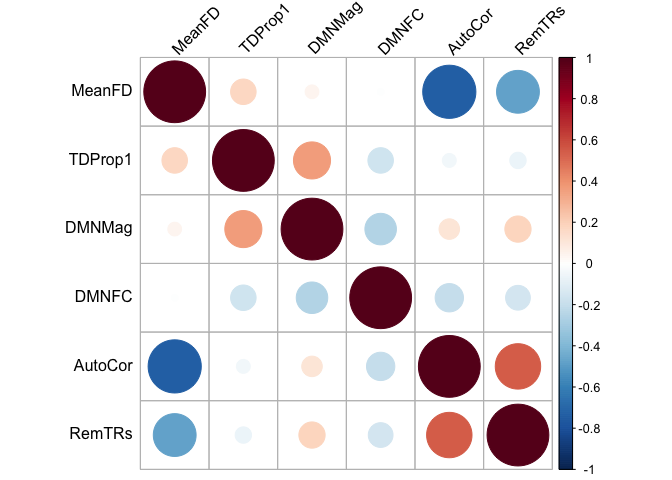
\includegraphics{Stats_n_Viz_files/figure-latex/unnamed-chunk-14-1.pdf}

\begin{Shaded}
\begin{Highlighting}[]
\FunctionTok{corrplot}\NormalTok{(}\FunctionTok{as.matrix}\NormalTok{(corrmatrix}\SpecialCharTok{$}\NormalTok{r),}\AttributeTok{method=}\StringTok{\textquotesingle{}number\textquotesingle{}}\NormalTok{)}
\end{Highlighting}
\end{Shaded}

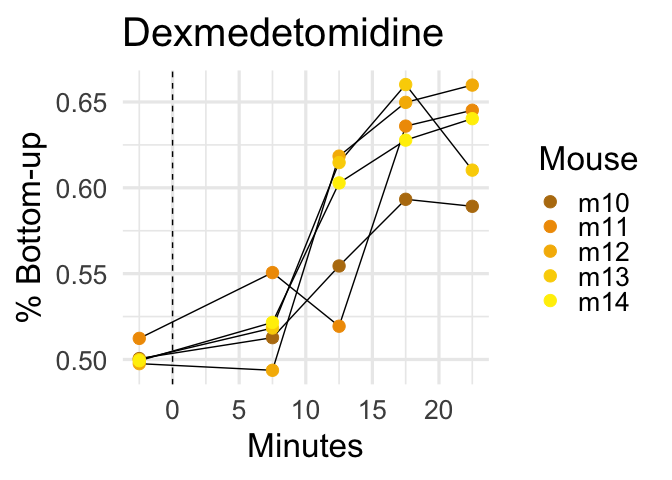
\includegraphics{Stats_n_Viz_files/figure-latex/unnamed-chunk-14-2.pdf}

\begin{Shaded}
\begin{Highlighting}[]
\CommentTok{\# need to establish which DMN metrics are associated above and beyond drug effect}
\CommentTok{\# DMN FC}
\NormalTok{dmnseg\_model }\OtherTok{\textless{}{-}} \FunctionTok{lme}\NormalTok{(DMNFC }\SpecialCharTok{\textasciitilde{}}\NormalTok{ MeanFD }\SpecialCharTok{+}\NormalTok{ Drug}\SpecialCharTok{+}\NormalTok{RemTRs}\SpecialCharTok{+}\NormalTok{Task}\SpecialCharTok{+}\NormalTok{TDProp1}\SpecialCharTok{+}\NormalTok{AutoCor}\SpecialCharTok{+}\NormalTok{DMNMag, }\AttributeTok{random =} \SpecialCharTok{\textasciitilde{}} \DecValTok{1} \SpecialCharTok{|}\NormalTok{ Subjects, }\AttributeTok{data =}\NormalTok{ mergedDfPropsComplAutoCdmnFCdmnMag)}
\CommentTok{\# DMN tdprops}
\NormalTok{td\_model }\OtherTok{\textless{}{-}} \FunctionTok{lme}\NormalTok{(TDProp1 }\SpecialCharTok{\textasciitilde{}}\NormalTok{ MeanFD }\SpecialCharTok{+}\NormalTok{ Drug}\SpecialCharTok{+}\NormalTok{RemTRs}\SpecialCharTok{+}\NormalTok{Task}\SpecialCharTok{+}\NormalTok{DMNFC}\SpecialCharTok{+}\NormalTok{AutoCor}\SpecialCharTok{+}\NormalTok{DMNMag, }\AttributeTok{random =} \SpecialCharTok{\textasciitilde{}} \DecValTok{1} \SpecialCharTok{|}\NormalTok{ Subjects, }\AttributeTok{data =}\NormalTok{ mergedDfPropsComplAutoCdmnFCdmnMag)}
\CommentTok{\# DMN Mag}
\NormalTok{dmnmag\_model }\OtherTok{\textless{}{-}} \FunctionTok{lme}\NormalTok{(DMNMag }\SpecialCharTok{\textasciitilde{}}\NormalTok{ MeanFD }\SpecialCharTok{+}\NormalTok{ Drug}\SpecialCharTok{+}\NormalTok{RemTRs}\SpecialCharTok{+}\NormalTok{Task}\SpecialCharTok{+}\NormalTok{DMNFC}\SpecialCharTok{+}\NormalTok{AutoCor}\SpecialCharTok{+}\NormalTok{TDProp1, }\AttributeTok{random =} \SpecialCharTok{\textasciitilde{}} \DecValTok{1} \SpecialCharTok{|}\NormalTok{ Subjects, }\AttributeTok{data =}\NormalTok{ mergedDfPropsComplAutoCdmnFCdmnMag)}
\CommentTok{\# DMN autocor}
\NormalTok{dmnAC\_model }\OtherTok{\textless{}{-}} \FunctionTok{lme}\NormalTok{(AutoCor }\SpecialCharTok{\textasciitilde{}}\NormalTok{ MeanFD }\SpecialCharTok{+}\NormalTok{ Drug}\SpecialCharTok{+}\NormalTok{RemTRs}\SpecialCharTok{+}\NormalTok{Task}\SpecialCharTok{+}\NormalTok{DMNFC}\SpecialCharTok{+}\NormalTok{DMNMag}\SpecialCharTok{+}\NormalTok{TDProp1, }\AttributeTok{random =} \SpecialCharTok{\textasciitilde{}} \DecValTok{1} \SpecialCharTok{|}\NormalTok{ Subjects, }\AttributeTok{data =}\NormalTok{ mergedDfPropsComplAutoCdmnFCdmnMag)}

\FunctionTok{library}\NormalTok{(pROC)}
\end{Highlighting}
\end{Shaded}

\begin{verbatim}
## Type 'citation("pROC")' for a citation.
\end{verbatim}

\begin{verbatim}
## 
## Attaching package: 'pROC'
\end{verbatim}

\begin{verbatim}
## The following objects are masked from 'package:stats':
## 
##     cov, smooth, var
\end{verbatim}

\begin{Shaded}
\begin{Highlighting}[]
\FunctionTok{library}\NormalTok{(plotROC)}
\end{Highlighting}
\end{Shaded}

\begin{verbatim}
## 
## Attaching package: 'plotROC'
\end{verbatim}

\begin{verbatim}
## The following object is masked from 'package:pROC':
## 
##     ggroc
\end{verbatim}

\begin{Shaded}
\begin{Highlighting}[]
\NormalTok{mergedDfPropsComplAutoCdmnFCdmnMag\_notask}\OtherTok{=}\NormalTok{mergedDfPropsComplAutoCdmnFCdmnMag[mergedDfPropsComplAutoCdmnFCdmnMag}\SpecialCharTok{$}\NormalTok{Task}\SpecialCharTok{==}\StringTok{\textquotesingle{}rs\textquotesingle{}}\NormalTok{,]}

\CommentTok{\# Fit logistic regression models}
\NormalTok{model1 }\OtherTok{\textless{}{-}} \FunctionTok{glm}\NormalTok{(Drug }\SpecialCharTok{\textasciitilde{}}\NormalTok{ MeanFD }\SpecialCharTok{+}\NormalTok{ RemTRs }\SpecialCharTok{+}\NormalTok{ DMNFC}\SpecialCharTok{+}\NormalTok{AutoCor, }\AttributeTok{data =}\NormalTok{ mergedDfPropsComplAutoCdmnFCdmnMag\_notask, }\AttributeTok{family =}\NormalTok{ binomial)}
\NormalTok{model2 }\OtherTok{\textless{}{-}} \FunctionTok{glm}\NormalTok{(Drug }\SpecialCharTok{\textasciitilde{}}\NormalTok{ MeanFD }\SpecialCharTok{+}\NormalTok{ RemTRs }\SpecialCharTok{+}\NormalTok{ DMNFC }\SpecialCharTok{+}\NormalTok{ AutoCor}\SpecialCharTok{+}\NormalTok{DMNMag}\SpecialCharTok{+}\NormalTok{TDProp1, }\AttributeTok{data =}\NormalTok{ mergedDfPropsComplAutoCdmnFCdmnMag\_notask, }\AttributeTok{family =}\NormalTok{ binomial)}

\CommentTok{\# Predict probabilities}
\NormalTok{prob1 }\OtherTok{\textless{}{-}} \FunctionTok{predict}\NormalTok{(model1, }\AttributeTok{type =} \StringTok{"response"}\NormalTok{)}
\NormalTok{prob2 }\OtherTok{\textless{}{-}} \FunctionTok{predict}\NormalTok{(model2, }\AttributeTok{type =} \StringTok{"response"}\NormalTok{)}

\CommentTok{\# Create a combined data frame for all models}
\NormalTok{df }\OtherTok{\textless{}{-}} \FunctionTok{data.frame}\NormalTok{(}
  \AttributeTok{labels =} \FunctionTok{as.numeric}\NormalTok{(}\FunctionTok{rep}\NormalTok{(mergedDfPropsComplAutoCdmnFCdmnMag\_notask}\SpecialCharTok{$}\NormalTok{Drug, }\DecValTok{2}\NormalTok{)),}
  \AttributeTok{predictions =} \FunctionTok{c}\NormalTok{(prob1, prob2),}
  \AttributeTok{model =} \FunctionTok{factor}\NormalTok{(}\FunctionTok{rep}\NormalTok{(}\FunctionTok{c}\NormalTok{(}\StringTok{"DMN Correlations"}\NormalTok{, }\StringTok{"+DMN Propagations"}\NormalTok{), }\AttributeTok{each =} \FunctionTok{nrow}\NormalTok{(mergedDfPropsComplAutoCdmnFCdmnMag\_notask)))}
\NormalTok{)}

\CommentTok{\# Generate the ROC plot}
\FunctionTok{ggplot}\NormalTok{(df, }\FunctionTok{aes}\NormalTok{(}\AttributeTok{m =}\NormalTok{ predictions, }\AttributeTok{d =}\NormalTok{ labels, }\AttributeTok{color =}\NormalTok{ model)) }\SpecialCharTok{+} 
  \FunctionTok{geom\_roc}\NormalTok{(}\AttributeTok{n.cuts =} \DecValTok{0}\NormalTok{, }\AttributeTok{labels =} \ConstantTok{FALSE}\NormalTok{) }\SpecialCharTok{+} 
  \FunctionTok{ylim}\NormalTok{(}\DecValTok{0}\NormalTok{, }\DecValTok{1}\NormalTok{) }\SpecialCharTok{+} \FunctionTok{ylab}\NormalTok{(}\StringTok{\textquotesingle{}True Positive Rate\textquotesingle{}}\NormalTok{) }\SpecialCharTok{+}\FunctionTok{xlab}\NormalTok{(}\StringTok{\textquotesingle{}False Positive Rate\textquotesingle{}}\NormalTok{)}\SpecialCharTok{+}
  \FunctionTok{ggtitle}\NormalTok{(}\StringTok{"ROC Curves for Classifying MDMA"}\NormalTok{) }\SpecialCharTok{+} 
  \FunctionTok{theme\_minimal}\NormalTok{(}\AttributeTok{base\_size=}\DecValTok{18}\NormalTok{) }\SpecialCharTok{+} 
  \FunctionTok{scale\_color\_manual}\NormalTok{(}\AttributeTok{values =} \FunctionTok{c}\NormalTok{(}\StringTok{"\#09416b"}\NormalTok{,}\StringTok{"\#c12139"}\NormalTok{))}\SpecialCharTok{+}
  \FunctionTok{geom\_abline}\NormalTok{(}\AttributeTok{intercept =} \DecValTok{0}\NormalTok{, }\AttributeTok{slope =} \DecValTok{1}\NormalTok{, }\AttributeTok{linetype =} \StringTok{"dashed"}\NormalTok{, }\AttributeTok{color =} \StringTok{"gray"}\NormalTok{)}\SpecialCharTok{+}
  \FunctionTok{theme}\NormalTok{(}\AttributeTok{legend.position =} \StringTok{"none"}\NormalTok{)}
\end{Highlighting}
\end{Shaded}

\begin{verbatim}
## Warning in verify_d(data$d): D not labeled 0/1, assuming 1 = 0 and 2 = 1!
\end{verbatim}

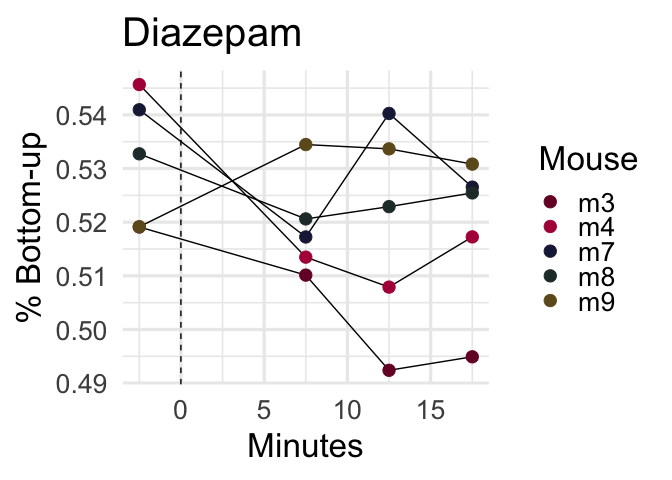
\includegraphics{Stats_n_Viz_files/figure-latex/unnamed-chunk-14-3.pdf}

\begin{Shaded}
\begin{Highlighting}[]
\CommentTok{\# Calculate AUC for each model}
\NormalTok{roc1 }\OtherTok{\textless{}{-}} \FunctionTok{roc}\NormalTok{(mergedDfPropsComplAutoCdmnFCdmnMag\_notask}\SpecialCharTok{$}\NormalTok{Drug, prob1)}
\end{Highlighting}
\end{Shaded}

\begin{verbatim}
## Setting levels: control = 0, case = 1
\end{verbatim}

\begin{verbatim}
## Setting direction: controls < cases
\end{verbatim}

\begin{Shaded}
\begin{Highlighting}[]
\NormalTok{roc2 }\OtherTok{\textless{}{-}} \FunctionTok{roc}\NormalTok{(mergedDfPropsComplAutoCdmnFCdmnMag\_notask}\SpecialCharTok{$}\NormalTok{Drug, prob2)}
\end{Highlighting}
\end{Shaded}

\begin{verbatim}
## Setting levels: control = 0, case = 1
## Setting direction: controls < cases
\end{verbatim}

\begin{Shaded}
\begin{Highlighting}[]
\CommentTok{\# Print AUC values}
\NormalTok{auc1 }\OtherTok{\textless{}{-}} \FunctionTok{auc}\NormalTok{(roc1)}
\NormalTok{auc2 }\OtherTok{\textless{}{-}} \FunctionTok{auc}\NormalTok{(roc2)}


\FunctionTok{print}\NormalTok{(}\FunctionTok{paste}\NormalTok{(}\StringTok{"AUC for DMN Correlations:"}\NormalTok{, auc1))}
\end{Highlighting}
\end{Shaded}

\begin{verbatim}
## [1] "AUC for DMN Correlations: 0.806481481481482"
\end{verbatim}

\begin{Shaded}
\begin{Highlighting}[]
\FunctionTok{print}\NormalTok{(}\FunctionTok{paste}\NormalTok{(}\StringTok{"AUC for Full Model:"}\NormalTok{, auc2))}
\end{Highlighting}
\end{Shaded}

\begin{verbatim}
## [1] "AUC for Full Model: 0.881481481481482"
\end{verbatim}

\begin{Shaded}
\begin{Highlighting}[]
\CommentTok{\# Calculate AUC difference between full and reduced models}
\NormalTok{auc\_diff }\OtherTok{\textless{}{-}}\NormalTok{ auc2 }\SpecialCharTok{{-}}\NormalTok{ auc1}
\end{Highlighting}
\end{Shaded}

\begin{Shaded}
\begin{Highlighting}[]
\CommentTok{\# Temporary comment out: output is making rstudio wonky}




\CommentTok{\# make equivalent AUC calculations on permuted data}
\CommentTok{\# initialize AUC difference vectors}
\CommentTok{\#auc\_diffs \textless{}{-} rep(NA, 1000)}
\CommentTok{\#}
\DocumentationTok{\#\# 1. permute each DMN variable (and FD)}
\CommentTok{\#set.seed(1)}
\CommentTok{\#for (i in 1:1000)\{}
\CommentTok{\#  print(i)}
\CommentTok{\#  \# permute DMNMag}
\CommentTok{\#  mergedDfPropsComplAutoCdmnFCdmnMag\_notask$DMNMag\_perm \textless{}{-} sample(mergedDfPropsComplAutoCdmnFCdmnMag\_notask$DMNMag)}
\CommentTok{\#  \# permute TDProp1}
\CommentTok{\#  mergedDfPropsComplAutoCdmnFCdmnMag\_notask$TDProp1\_perm \textless{}{-} sample(mergedDfPropsComplAutoCdmnFCdmnMag\_notask$TDProp1)}
\CommentTok{\# }
\CommentTok{\#  \# Fit logistic regression models}
\CommentTok{\#  model1 \textless{}{-} glm(Drug \textasciitilde{} MeanFD + RemTRs + DMNFC+AutoCor, data = mergedDfPropsComplAutoCdmnFCdmnMag\_notask, family = \#binomial)}
\CommentTok{\#  model2\_perm \textless{}{-} glm(Drug \textasciitilde{} MeanFD + RemTRs + DMNFC+AutoCor+TDProp1\_perm+DMNMag\_perm, data = \#mergedDfPropsComplAutoCdmnFCdmnMag\_notask, family = binomial)}
\CommentTok{\#   }
\CommentTok{\#  \# 3. calculate AUC difference between full and reduced models with permuted data}
\CommentTok{\#  roc1 \textless{}{-} roc(mergedDfPropsComplAutoCdmnFCdmnMag\_notask$Drug, predict(model1, type = "response"))}
\CommentTok{\#  roc2\_perm \textless{}{-} roc(mergedDfPropsComplAutoCdmnFCdmnMag\_notask$Drug, predict(model2\_perm, type = "response"))}
\CommentTok{\#  }
\CommentTok{\#  \# Print AUC values}
\CommentTok{\#  auc1 \textless{}{-} auc(roc1)}
\CommentTok{\#  auc2\_perm \textless{}{-}auc(roc2\_perm)}
\CommentTok{\#}
\CommentTok{\#  \# populate auc\_diff vectors}
\CommentTok{\#  \# DMN correlations vs. full (permuted props) model}
\CommentTok{\#  auc\_diffs[i] \textless{}{-} auc1 {-} auc2\_perm}
\CommentTok{\#\}}
\DocumentationTok{\#\# 4. Compare true AUC differences to permuted AUC differences}
\CommentTok{\#}
\CommentTok{\#sum(auc\_diffs\textgreater{}auc\_diff)}
\CommentTok{\# 0 indicates p \textless{}0.001}
\end{Highlighting}
\end{Shaded}

\begin{Shaded}
\begin{Highlighting}[]
\CommentTok{\# great, now let\textquotesingle{}s bootstrap them}
\CommentTok{\# Set the number of bootstrap samples}
\NormalTok{num\_bootstrap\_samples }\OtherTok{\textless{}{-}} \DecValTok{1000}
\CommentTok{\# initialize t vectors}
\NormalTok{td\_d}\OtherTok{\textless{}{-}}\FunctionTok{rep}\NormalTok{(}\DecValTok{0}\NormalTok{,num\_bootstrap\_samples)}
\NormalTok{td\_fd}\OtherTok{\textless{}{-}}\FunctionTok{rep}\NormalTok{(}\DecValTok{0}\NormalTok{,num\_bootstrap\_samples)}
\NormalTok{ta\_d}\OtherTok{\textless{}{-}}\FunctionTok{rep}\NormalTok{(}\DecValTok{0}\NormalTok{,num\_bootstrap\_samples)}
\NormalTok{ta\_fd}\OtherTok{\textless{}{-}}\FunctionTok{rep}\NormalTok{(}\DecValTok{0}\NormalTok{,num\_bootstrap\_samples)}
\NormalTok{ds\_d}\OtherTok{\textless{}{-}}\FunctionTok{rep}\NormalTok{(}\DecValTok{0}\NormalTok{,num\_bootstrap\_samples)}
\NormalTok{ds\_fd}\OtherTok{\textless{}{-}}\FunctionTok{rep}\NormalTok{(}\DecValTok{0}\NormalTok{,num\_bootstrap\_samples)}
\NormalTok{dm\_d}\OtherTok{\textless{}{-}}\FunctionTok{rep}\NormalTok{(}\DecValTok{0}\NormalTok{,num\_bootstrap\_samples)}
\NormalTok{dm\_fd}\OtherTok{\textless{}{-}}\FunctionTok{rep}\NormalTok{(}\DecValTok{0}\NormalTok{,num\_bootstrap\_samples)}

\CommentTok{\# bootstrap loops}
\FunctionTok{set.seed}\NormalTok{(}\DecValTok{1}\NormalTok{)}
\ControlFlowTok{for}\NormalTok{ (i }\ControlFlowTok{in} \DecValTok{1}\SpecialCharTok{:}\NormalTok{num\_bootstrap\_samples)\{}
  \CommentTok{\# resample data}
\NormalTok{  data}\OtherTok{=}\NormalTok{mergedDfPropsComplAutoCdmnFCdmnMag[}\FunctionTok{sample}\NormalTok{(}\FunctionTok{nrow}\NormalTok{(mergedDfPropsComplAutoCdmnFCdmnMag), }\AttributeTok{replace =} \ConstantTok{TRUE}\NormalTok{), ]}
  \CommentTok{\# fit on all models}
\NormalTok{  td\_model }\OtherTok{\textless{}{-}} \FunctionTok{lme}\NormalTok{(TDProp1 }\SpecialCharTok{\textasciitilde{}}\NormalTok{ MeanFD }\SpecialCharTok{+}\NormalTok{ Drug}\SpecialCharTok{+}\NormalTok{RemTRs}\SpecialCharTok{+}\NormalTok{Task, }\AttributeTok{random =} \SpecialCharTok{\textasciitilde{}} \DecValTok{1} \SpecialCharTok{|}\NormalTok{ Subjects, }\AttributeTok{data =}\NormalTok{ data)}
\NormalTok{  ta\_model }\OtherTok{\textless{}{-}} \FunctionTok{lme}\NormalTok{(AutoCor }\SpecialCharTok{\textasciitilde{}}\NormalTok{ MeanFD }\SpecialCharTok{+}\NormalTok{ Drug}\SpecialCharTok{+}\NormalTok{RemTRs}\SpecialCharTok{+}\NormalTok{Task, }\AttributeTok{random =} \SpecialCharTok{\textasciitilde{}} \DecValTok{1} \SpecialCharTok{|}\NormalTok{ Subjects, }\AttributeTok{data =}\NormalTok{ data)}
\NormalTok{  ds\_model }\OtherTok{\textless{}{-}} \FunctionTok{lme}\NormalTok{(DMNFC }\SpecialCharTok{\textasciitilde{}}\NormalTok{ MeanFD }\SpecialCharTok{+}\NormalTok{ Drug}\SpecialCharTok{+}\NormalTok{RemTRs}\SpecialCharTok{+}\NormalTok{Task, }\AttributeTok{random =} \SpecialCharTok{\textasciitilde{}} \DecValTok{1} \SpecialCharTok{|}\NormalTok{ Subjects, }\AttributeTok{data =}\NormalTok{ data)}
\NormalTok{  dm\_model }\OtherTok{\textless{}{-}} \FunctionTok{lme}\NormalTok{(DMNMag }\SpecialCharTok{\textasciitilde{}}\NormalTok{ MeanFD }\SpecialCharTok{+}\NormalTok{ Drug}\SpecialCharTok{+}\NormalTok{RemTRs}\SpecialCharTok{+}\NormalTok{Task, }\AttributeTok{random =} \SpecialCharTok{\textasciitilde{}} \DecValTok{1} \SpecialCharTok{|}\NormalTok{ Subjects, }\AttributeTok{data =}\NormalTok{ data)}
  \CommentTok{\# get t{-}values}
\NormalTok{  td\_d[i]}\OtherTok{=}\FunctionTok{summary}\NormalTok{(td\_model)}\SpecialCharTok{$}\NormalTok{tTable[}\FunctionTok{rownames}\NormalTok{(}\FunctionTok{summary}\NormalTok{(td\_model)}\SpecialCharTok{$}\NormalTok{tTable) }\SpecialCharTok{==} \StringTok{"Drug1"}\NormalTok{, }\StringTok{"t{-}value"}\NormalTok{]}
\NormalTok{  td\_fd[i]}\OtherTok{=}\FunctionTok{summary}\NormalTok{(td\_model)}\SpecialCharTok{$}\NormalTok{tTable[}\FunctionTok{rownames}\NormalTok{(}\FunctionTok{summary}\NormalTok{(td\_model)}\SpecialCharTok{$}\NormalTok{tTable) }\SpecialCharTok{==} \StringTok{"MeanFD"}\NormalTok{, }\StringTok{"t{-}value"}\NormalTok{]}
\NormalTok{  ta\_d[i]}\OtherTok{=}\FunctionTok{summary}\NormalTok{(ta\_model)}\SpecialCharTok{$}\NormalTok{tTable[}\FunctionTok{rownames}\NormalTok{(}\FunctionTok{summary}\NormalTok{(ta\_model)}\SpecialCharTok{$}\NormalTok{tTable) }\SpecialCharTok{==} \StringTok{"Drug1"}\NormalTok{, }\StringTok{"t{-}value"}\NormalTok{]}
\NormalTok{  ta\_fd[i]}\OtherTok{=}\FunctionTok{summary}\NormalTok{(ta\_model)}\SpecialCharTok{$}\NormalTok{tTable[}\FunctionTok{rownames}\NormalTok{(}\FunctionTok{summary}\NormalTok{(ta\_model)}\SpecialCharTok{$}\NormalTok{tTable) }\SpecialCharTok{==} \StringTok{"MeanFD"}\NormalTok{, }\StringTok{"t{-}value"}\NormalTok{]}
\NormalTok{  ds\_d[i]}\OtherTok{=}\FunctionTok{summary}\NormalTok{(ds\_model)}\SpecialCharTok{$}\NormalTok{tTable[}\FunctionTok{rownames}\NormalTok{(}\FunctionTok{summary}\NormalTok{(ds\_model)}\SpecialCharTok{$}\NormalTok{tTable) }\SpecialCharTok{==} \StringTok{"Drug1"}\NormalTok{, }\StringTok{"t{-}value"}\NormalTok{]}
\NormalTok{  ds\_fd[i]}\OtherTok{=}\FunctionTok{summary}\NormalTok{(ds\_model)}\SpecialCharTok{$}\NormalTok{tTable[}\FunctionTok{rownames}\NormalTok{(}\FunctionTok{summary}\NormalTok{(ds\_model)}\SpecialCharTok{$}\NormalTok{tTable) }\SpecialCharTok{==} \StringTok{"MeanFD"}\NormalTok{, }\StringTok{"t{-}value"}\NormalTok{]}
\NormalTok{  dm\_d[i]}\OtherTok{=}\FunctionTok{summary}\NormalTok{(dm\_model)}\SpecialCharTok{$}\NormalTok{tTable[}\FunctionTok{rownames}\NormalTok{(}\FunctionTok{summary}\NormalTok{(dm\_model)}\SpecialCharTok{$}\NormalTok{tTable) }\SpecialCharTok{==} \StringTok{"Drug1"}\NormalTok{, }\StringTok{"t{-}value"}\NormalTok{]}
\NormalTok{  dm\_fd[i]}\OtherTok{=}\FunctionTok{summary}\NormalTok{(dm\_model)}\SpecialCharTok{$}\NormalTok{tTable[}\FunctionTok{rownames}\NormalTok{(}\FunctionTok{summary}\NormalTok{(dm\_model)}\SpecialCharTok{$}\NormalTok{tTable) }\SpecialCharTok{==} \StringTok{"MeanFD"}\NormalTok{, }\StringTok{"t{-}value"}\NormalTok{]}
\NormalTok{\}}
\CommentTok{\# convert to dataframes}
\NormalTok{td\_d}\OtherTok{=}\FunctionTok{data.frame}\NormalTok{(td\_d)}
\NormalTok{ta\_d}\OtherTok{=}\FunctionTok{data.frame}\NormalTok{(ta\_d)}
\NormalTok{ds\_d}\OtherTok{=}\FunctionTok{data.frame}\NormalTok{(ds\_d)}
\NormalTok{dm\_d}\OtherTok{=}\FunctionTok{data.frame}\NormalTok{(dm\_d)}
\NormalTok{td\_fd}\OtherTok{=}\FunctionTok{data.frame}\NormalTok{(td\_fd)}
\NormalTok{ta\_fd}\OtherTok{=}\FunctionTok{data.frame}\NormalTok{(ta\_fd)}
\NormalTok{ds\_fd}\OtherTok{=}\FunctionTok{data.frame}\NormalTok{(ds\_fd)}
\NormalTok{dm\_fd}\OtherTok{=}\FunctionTok{data.frame}\NormalTok{(dm\_fd)}

\FunctionTok{colnames}\NormalTok{(td\_d)}\OtherTok{=}\StringTok{\textquotesingle{}tstat\textquotesingle{}}
\FunctionTok{colnames}\NormalTok{(ta\_d)}\OtherTok{=}\StringTok{\textquotesingle{}tstat\textquotesingle{}}
\FunctionTok{colnames}\NormalTok{(ds\_d)}\OtherTok{=}\StringTok{\textquotesingle{}tstat\textquotesingle{}}
\FunctionTok{colnames}\NormalTok{(dm\_d)}\OtherTok{=}\StringTok{\textquotesingle{}tstat\textquotesingle{}}
\FunctionTok{colnames}\NormalTok{(td\_fd)}\OtherTok{=}\StringTok{\textquotesingle{}tstat\textquotesingle{}}
\FunctionTok{colnames}\NormalTok{(ta\_fd)}\OtherTok{=}\StringTok{\textquotesingle{}tstat\textquotesingle{}}
\FunctionTok{colnames}\NormalTok{(ds\_fd)}\OtherTok{=}\StringTok{\textquotesingle{}tstat\textquotesingle{}}
\FunctionTok{colnames}\NormalTok{(dm\_fd)}\OtherTok{=}\StringTok{\textquotesingle{}tstat\textquotesingle{}}

\CommentTok{\# set column names for merging}
\NormalTok{td\_d}\SpecialCharTok{$}\NormalTok{Cov}\OtherTok{=}\StringTok{\textquotesingle{}Drug\textquotesingle{}}
\NormalTok{ta\_d}\SpecialCharTok{$}\NormalTok{Cov}\OtherTok{=}\StringTok{\textquotesingle{}Drug\textquotesingle{}}
\NormalTok{ds\_d}\SpecialCharTok{$}\NormalTok{Cov}\OtherTok{=}\StringTok{\textquotesingle{}Drug\textquotesingle{}}
\NormalTok{dm\_d}\SpecialCharTok{$}\NormalTok{Cov}\OtherTok{=}\StringTok{\textquotesingle{}Drug\textquotesingle{}}

\NormalTok{td\_fd}\SpecialCharTok{$}\NormalTok{Cov}\OtherTok{=}\StringTok{\textquotesingle{}FD\textquotesingle{}}
\NormalTok{ta\_fd}\SpecialCharTok{$}\NormalTok{Cov}\OtherTok{=}\StringTok{\textquotesingle{}FD\textquotesingle{}}
\NormalTok{ds\_fd}\SpecialCharTok{$}\NormalTok{Cov}\OtherTok{=}\StringTok{\textquotesingle{}FD\textquotesingle{}}
\NormalTok{dm\_fd}\SpecialCharTok{$}\NormalTok{Cov}\OtherTok{=}\StringTok{\textquotesingle{}FD\textquotesingle{}}

\NormalTok{td\_d}\SpecialCharTok{$}\NormalTok{Model}\OtherTok{=}\StringTok{\textquotesingle{}Bottom{-}up \%\textquotesingle{}}
\NormalTok{ta\_d}\SpecialCharTok{$}\NormalTok{Model}\OtherTok{=}\StringTok{\textquotesingle{}AutoCor\textquotesingle{}}
\NormalTok{ds\_d}\SpecialCharTok{$}\NormalTok{Model}\OtherTok{=}\StringTok{\textquotesingle{}Integration\textquotesingle{}}
\NormalTok{dm\_d}\SpecialCharTok{$}\NormalTok{Model}\OtherTok{=}\StringTok{\textquotesingle{}Magnitude\textquotesingle{}}

\NormalTok{td\_fd}\SpecialCharTok{$}\NormalTok{Model}\OtherTok{=}\StringTok{\textquotesingle{}Bottom{-}up \%\textquotesingle{}}
\NormalTok{ta\_fd}\SpecialCharTok{$}\NormalTok{Model}\OtherTok{=}\StringTok{\textquotesingle{}AutoCor\textquotesingle{}}
\NormalTok{ds\_fd}\SpecialCharTok{$}\NormalTok{Model}\OtherTok{=}\StringTok{\textquotesingle{}Integration\textquotesingle{}}
\NormalTok{dm\_fd}\SpecialCharTok{$}\NormalTok{Model}\OtherTok{=}\StringTok{\textquotesingle{}Magnitude\textquotesingle{}}

\NormalTok{bootstrap\_results\_FD}\OtherTok{=}\FunctionTok{rbind}\NormalTok{(td\_fd,ta\_fd,ds\_fd,dm\_fd)}
\NormalTok{bootstrap\_results\_Drug}\OtherTok{=}\FunctionTok{rbind}\NormalTok{(td\_d,ta\_d,ds\_d,dm\_d)}
\CommentTok{\# Calculate the average t{-}value for each Model category}
\NormalTok{average\_t\_values }\OtherTok{\textless{}{-}}\NormalTok{ bootstrap\_results\_FD }\SpecialCharTok{\%\textgreater{}\%}
  \FunctionTok{group\_by}\NormalTok{(Model) }\SpecialCharTok{\%\textgreater{}\%}
  \FunctionTok{summarize}\NormalTok{(}\AttributeTok{avg\_t\_value =} \FunctionTok{mean}\NormalTok{(}\FunctionTok{abs}\NormalTok{(tstat), }\AttributeTok{na.rm =} \ConstantTok{TRUE}\NormalTok{))}

\CommentTok{\# Reorder the Model factor based on the average t{-}values}
\NormalTok{bootstrap\_results\_FD}\SpecialCharTok{$}\NormalTok{Model }\OtherTok{\textless{}{-}} \FunctionTok{factor}\NormalTok{(bootstrap\_results\_FD}\SpecialCharTok{$}\NormalTok{Model, }
                                     \AttributeTok{levels =}\NormalTok{ average\_t\_values}\SpecialCharTok{$}\NormalTok{Model[}\FunctionTok{order}\NormalTok{(average\_t\_values}\SpecialCharTok{$}\NormalTok{avg\_t\_value)])}


\CommentTok{\# Calculate the average t{-}value for each Model category}
\NormalTok{average\_t\_values }\OtherTok{\textless{}{-}}\NormalTok{ bootstrap\_results\_Drug }\SpecialCharTok{\%\textgreater{}\%}
  \FunctionTok{group\_by}\NormalTok{(Model) }\SpecialCharTok{\%\textgreater{}\%}
  \FunctionTok{summarize}\NormalTok{(}\AttributeTok{avg\_t\_value =} \FunctionTok{mean}\NormalTok{(}\FunctionTok{abs}\NormalTok{(tstat), }\AttributeTok{na.rm =} \ConstantTok{TRUE}\NormalTok{))}

\CommentTok{\# Reorder the Model factor based on the average t{-}values}
\NormalTok{bootstrap\_results\_Drug}\SpecialCharTok{$}\NormalTok{Model }\OtherTok{\textless{}{-}} \FunctionTok{factor}\NormalTok{(bootstrap\_results\_Drug}\SpecialCharTok{$}\NormalTok{Model, }
                                     \AttributeTok{levels =}\NormalTok{ average\_t\_values}\SpecialCharTok{$}\NormalTok{Model[}\FunctionTok{order}\NormalTok{(average\_t\_values}\SpecialCharTok{$}\NormalTok{avg\_t\_value)])}

\FunctionTok{library}\NormalTok{(ggdist)}
\CommentTok{\# Generate the plot}
\FunctionTok{ggplot}\NormalTok{(bootstrap\_results\_FD, }\FunctionTok{aes}\NormalTok{(}\AttributeTok{x =}\NormalTok{ Model, }\AttributeTok{y =}\NormalTok{ tstat, }\AttributeTok{fill =}\NormalTok{ Cov)) }\SpecialCharTok{+}
    \FunctionTok{geom\_boxplot}\NormalTok{(}
        \AttributeTok{width =} \FloatTok{0.12}\NormalTok{,}
        \CommentTok{\# Removing outliers}
        \AttributeTok{outlier.color =} \ConstantTok{NA}\NormalTok{,}
        \AttributeTok{fill=}\StringTok{\textquotesingle{}\#EF9500\textquotesingle{}}
\NormalTok{    ) }\SpecialCharTok{+}
    \FunctionTok{stat\_dots}\NormalTok{(}
        \CommentTok{\# Plotting on left side}
        \AttributeTok{side =} \StringTok{"left"}\NormalTok{,}
        \CommentTok{\# Adjusting position}
        \AttributeTok{justification =} \FloatTok{1.1}\NormalTok{,}
        \CommentTok{\# Adjust grouping (binning) of observations}
        \AttributeTok{binwidth =} \FloatTok{0.08}
\NormalTok{    ) }\SpecialCharTok{+}
    \FunctionTok{labs}\NormalTok{(}\AttributeTok{x =} \StringTok{"Model"}\NormalTok{, }\AttributeTok{y =} \StringTok{"T{-}Values"}\NormalTok{, }\AttributeTok{title =} \StringTok{"Bootstrap T{-}Values for FD effect"}\NormalTok{) }\SpecialCharTok{+}
    \FunctionTok{theme\_minimal}\NormalTok{(}\AttributeTok{base\_size =} \DecValTok{18}\NormalTok{) }\SpecialCharTok{+}
    \FunctionTok{geom\_hline}\NormalTok{(}\AttributeTok{yintercept =} \DecValTok{0}\NormalTok{, }\AttributeTok{linetype =} \StringTok{"dashed"}\NormalTok{)}\SpecialCharTok{+}
    \CommentTok{\# just to prevent extra x{-}axis expansion}
    \FunctionTok{coord\_cartesian}\NormalTok{(}\AttributeTok{xlim =} \FunctionTok{c}\NormalTok{(.}\DecValTok{8}\NormalTok{, }\FunctionTok{length}\NormalTok{(}\FunctionTok{unique}\NormalTok{(bootstrap\_results\_Drug}\SpecialCharTok{$}\NormalTok{Model))))}\SpecialCharTok{+}
    \FunctionTok{theme}\NormalTok{(}\AttributeTok{legend.position =} \StringTok{"none"}\NormalTok{)}
\end{Highlighting}
\end{Shaded}

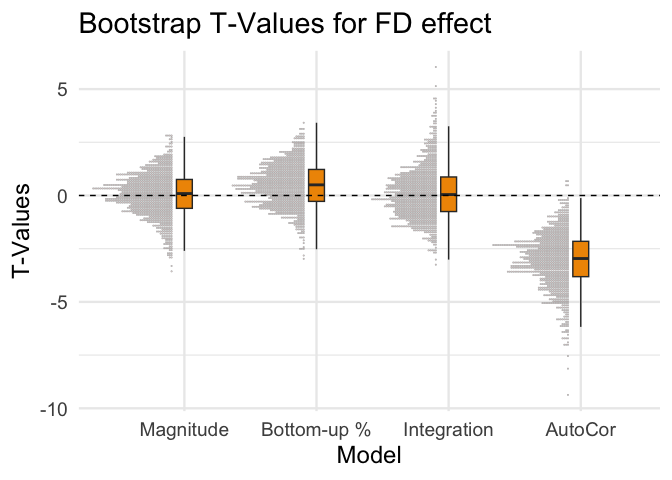
\includegraphics{Stats_n_Viz_files/figure-latex/unnamed-chunk-16-1.pdf}

\begin{Shaded}
\begin{Highlighting}[]
\CommentTok{\# Calculate the average t{-}value for each Model category}
\NormalTok{average\_t\_values }\OtherTok{\textless{}{-}}\NormalTok{ bootstrap\_results\_Drug }\SpecialCharTok{\%\textgreater{}\%}
  \FunctionTok{group\_by}\NormalTok{(Model) }\SpecialCharTok{\%\textgreater{}\%}
  \FunctionTok{summarize}\NormalTok{(}\AttributeTok{avg\_t\_value =} \FunctionTok{mean}\NormalTok{(tstat, }\AttributeTok{na.rm =} \ConstantTok{TRUE}\NormalTok{))}

\CommentTok{\# Reorder the Model factor based on the average t{-}values}
\NormalTok{bootstrap\_results\_Drug}\SpecialCharTok{$}\NormalTok{Model }\OtherTok{\textless{}{-}} \FunctionTok{factor}\NormalTok{(bootstrap\_results\_Drug}\SpecialCharTok{$}\NormalTok{Model, }
                                     \AttributeTok{levels =} \FunctionTok{c}\NormalTok{(}\StringTok{\textquotesingle{}Integration\textquotesingle{}}\NormalTok{,}\StringTok{\textquotesingle{}AutoCor\textquotesingle{}}\NormalTok{,}\StringTok{\textquotesingle{}Bottom{-}up \%\textquotesingle{}}\NormalTok{,}\StringTok{\textquotesingle{}Magnitude\textquotesingle{}}\NormalTok{))}


\CommentTok{\# add fill column}
\NormalTok{bootstrap\_results\_Drug}\SpecialCharTok{$}\NormalTok{Fill}\OtherTok{=}\StringTok{\textquotesingle{}DMN Correlatons\textquotesingle{}}
\NormalTok{bootstrap\_results\_Drug}\SpecialCharTok{$}\NormalTok{Fill[bootstrap\_results\_Drug}\SpecialCharTok{$}\NormalTok{Model}\SpecialCharTok{==}\StringTok{\textquotesingle{}Bottom{-}up \%\textquotesingle{}}\NormalTok{]}\OtherTok{=}\StringTok{\textquotesingle{}DMN Propagations\textquotesingle{}}
\NormalTok{bootstrap\_results\_Drug}\SpecialCharTok{$}\NormalTok{Fill[bootstrap\_results\_Drug}\SpecialCharTok{$}\NormalTok{Model}\SpecialCharTok{==}\StringTok{\textquotesingle{}Magnitude\textquotesingle{}}\NormalTok{]}\OtherTok{=}\StringTok{\textquotesingle{}DMN Propagations\textquotesingle{}}


\CommentTok{\# Generate the plot}
\FunctionTok{ggplot}\NormalTok{(bootstrap\_results\_Drug, }\FunctionTok{aes}\NormalTok{(}\AttributeTok{x =}\NormalTok{ Model, }\AttributeTok{y =}\NormalTok{ tstat, }\AttributeTok{fill =}\NormalTok{ Fill)) }\SpecialCharTok{+}
    \FunctionTok{geom\_boxplot}\NormalTok{(}
        \AttributeTok{width =} \FloatTok{0.12}\NormalTok{,}
        \CommentTok{\# Removing outliers}
        \AttributeTok{outlier.color =} \ConstantTok{NA}\NormalTok{) }\SpecialCharTok{+}
        \FunctionTok{scale\_fill\_manual}\NormalTok{(}\AttributeTok{values=}\FunctionTok{c}\NormalTok{(}\StringTok{"\#c12139"}\NormalTok{,}\StringTok{"\#09416b"}\NormalTok{))}\SpecialCharTok{+}
    \FunctionTok{stat\_dots}\NormalTok{(}
        \CommentTok{\# Plotting on left side}
        \AttributeTok{side =} \StringTok{"left"}\NormalTok{,}
        \CommentTok{\# Adjusting position}
        \AttributeTok{justification =} \FloatTok{1.1}\NormalTok{,}
        \CommentTok{\# Adjust grouping (binning) of observations}
        \AttributeTok{binwidth =} \FloatTok{0.08}\NormalTok{,}
        \AttributeTok{overflow =} \StringTok{"compress"}
\NormalTok{    ) }\SpecialCharTok{+}
    \FunctionTok{labs}\NormalTok{(}\AttributeTok{x =} \StringTok{"Model"}\NormalTok{, }\AttributeTok{y =} \StringTok{"T{-}Values"}\NormalTok{, }\AttributeTok{title =} \StringTok{"Bootstrap T{-}Values for MDMA effect"}\NormalTok{) }\SpecialCharTok{+}
    \FunctionTok{theme\_minimal}\NormalTok{(}\AttributeTok{base\_size =} \DecValTok{18}\NormalTok{) }\SpecialCharTok{+}
    \FunctionTok{geom\_hline}\NormalTok{(}\AttributeTok{yintercept =} \DecValTok{0}\NormalTok{, }\AttributeTok{linetype =} \StringTok{"dashed"}\NormalTok{)}\SpecialCharTok{+}
    \CommentTok{\# just to prevent extra x{-}axis expansion}
    \FunctionTok{coord\_cartesian}\NormalTok{(}\AttributeTok{xlim =} \FunctionTok{c}\NormalTok{(}\DecValTok{1}\NormalTok{, }\FunctionTok{length}\NormalTok{(}\FunctionTok{unique}\NormalTok{(bootstrap\_results\_Drug}\SpecialCharTok{$}\NormalTok{Model))))}\SpecialCharTok{+}
    \FunctionTok{theme}\NormalTok{(}\AttributeTok{legend.position =} \StringTok{"none"}\NormalTok{)}\SpecialCharTok{+}\FunctionTok{ylim}\NormalTok{(}\FunctionTok{c}\NormalTok{(}\SpecialCharTok{{-}}\FloatTok{10.5}\NormalTok{,}\FloatTok{10.5}\NormalTok{))}
\end{Highlighting}
\end{Shaded}

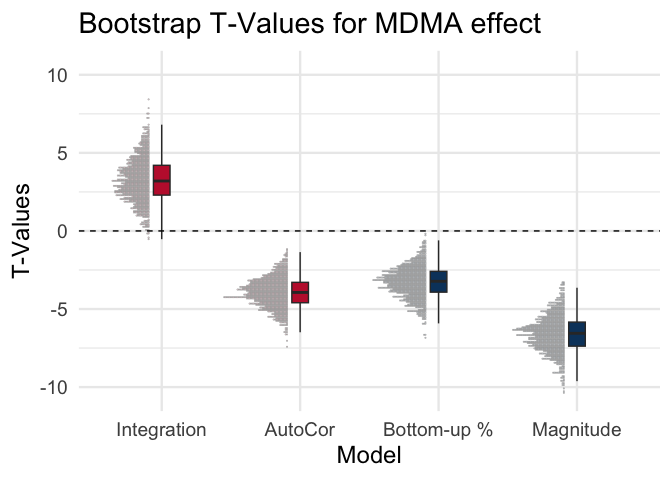
\includegraphics{Stats_n_Viz_files/figure-latex/unnamed-chunk-16-2.pdf}

\begin{Shaded}
\begin{Highlighting}[]
\CommentTok{\# now compare with VAS}
\NormalTok{vas}\OtherTok{=}\FunctionTok{read.csv}\NormalTok{(}\StringTok{\textquotesingle{}\textasciitilde{}/Downloads/MDMA\_VAS\_ASC\_forAdam\_03062023.csv\textquotesingle{}}\NormalTok{)}
\CommentTok{\# correct subject naming}
\NormalTok{vas}\SpecialCharTok{$}\NormalTok{Subjects }\OtherTok{\textless{}{-}} \FunctionTok{paste0}\NormalTok{(}\StringTok{"sub{-}MDMA"}\NormalTok{, }\FunctionTok{sprintf}\NormalTok{(}\StringTok{"\%03d"}\NormalTok{, vas}\SpecialCharTok{$}\NormalTok{Subjects))}
\NormalTok{VASmerge}\OtherTok{=}\FunctionTok{merge}\NormalTok{(vas,mergedDfPropsComplAutoCdmnFCdmnMag,}\AttributeTok{by=}\FunctionTok{c}\NormalTok{(}\StringTok{"Subjects"}\NormalTok{,}\StringTok{"Dosage"}\NormalTok{))}
\end{Highlighting}
\end{Shaded}

\begin{Shaded}
\begin{Highlighting}[]
\DocumentationTok{\#\#\#\#\#\# spin tests}
\CommentTok{\# load in y7 alignment left}
\NormalTok{y7align\_L}\OtherTok{=}\FunctionTok{read.csv}\NormalTok{(}\StringTok{\textquotesingle{}\textasciitilde{}/Downloads/perm\_vs\_obs\_DMN\_Y7\_L.csv\textquotesingle{}}\NormalTok{)}
\NormalTok{y7align\_R}\OtherTok{=}\FunctionTok{read.csv}\NormalTok{(}\StringTok{\textquotesingle{}\textasciitilde{}/Downloads/perm\_vs\_obs\_DMN\_Y7\_R.csv\textquotesingle{}}\NormalTok{)}
\CommentTok{\# add a real vs. permuted value}
\NormalTok{y7align\_L}\SpecialCharTok{$}\NormalTok{Observed}\OtherTok{=}\DecValTok{0}
\NormalTok{y7align\_R}\SpecialCharTok{$}\NormalTok{Observed}\OtherTok{=}\DecValTok{0}
\NormalTok{y7align\_L}\SpecialCharTok{$}\NormalTok{Observed[}\DecValTok{10001}\NormalTok{]}\OtherTok{=}\DecValTok{1}
\NormalTok{y7align\_R}\SpecialCharTok{$}\NormalTok{Observed[}\DecValTok{10001}\NormalTok{]}\OtherTok{=}\DecValTok{1}
\CommentTok{\# add right vs. left}
\NormalTok{y7align\_L}\SpecialCharTok{$}\NormalTok{Side}\OtherTok{=}\StringTok{\textquotesingle{}Left\textquotesingle{}}
\NormalTok{y7align\_R}\SpecialCharTok{$}\NormalTok{Side}\OtherTok{=}\StringTok{\textquotesingle{}Right\textquotesingle{}}
\NormalTok{y7plotdf}\OtherTok{=}\FunctionTok{rbind}\NormalTok{(y7align\_L,y7align\_R)}

\CommentTok{\# subset spun and nonspun df}
\NormalTok{spunL}\OtherTok{=}\NormalTok{y7align\_L[}\DecValTok{1}\SpecialCharTok{:}\DecValTok{10000}\NormalTok{,]}
\NormalTok{ObsL}\OtherTok{=}\NormalTok{y7align\_L[}\DecValTok{10001}\NormalTok{,]}
\NormalTok{spunR}\OtherTok{=}\NormalTok{y7align\_R[}\DecValTok{1}\SpecialCharTok{:}\DecValTok{10000}\NormalTok{,]}
\NormalTok{ObsR}\OtherTok{=}\NormalTok{y7align\_R[}\DecValTok{10001}\NormalTok{,]}
  
\CommentTok{\# left hemi}
\FunctionTok{ggplot}\NormalTok{(spunL,}\FunctionTok{aes}\NormalTok{(}\AttributeTok{x=}\NormalTok{Var1))}\SpecialCharTok{+}\FunctionTok{geom\_density}\NormalTok{(}\AttributeTok{size=}\FloatTok{1.5}\NormalTok{)}\SpecialCharTok{+}\FunctionTok{geom\_vline}\NormalTok{(}\AttributeTok{xintercept =}\NormalTok{ ObsL}\SpecialCharTok{$}\NormalTok{Var1,}\AttributeTok{size=}\DecValTok{2}\NormalTok{,}\AttributeTok{color=}\StringTok{\textquotesingle{}\#BC3754\textquotesingle{}}\NormalTok{)}\SpecialCharTok{+}\FunctionTok{theme\_classic}\NormalTok{(}\AttributeTok{base\_size=}\DecValTok{23}\NormalTok{)}\SpecialCharTok{+}\FunctionTok{ylab}\NormalTok{(}\StringTok{\textquotesingle{}\textquotesingle{}}\NormalTok{)}\SpecialCharTok{+}\FunctionTok{xlab}\NormalTok{(}\StringTok{\textquotesingle{}T{-}Statistics\textquotesingle{}}\NormalTok{)}\SpecialCharTok{+}\FunctionTok{guides}\NormalTok{(}\AttributeTok{y=}\StringTok{"none"}\NormalTok{)}\SpecialCharTok{+}\FunctionTok{theme}\NormalTok{(}\AttributeTok{axis.text =} \FunctionTok{element\_text}\NormalTok{(}\AttributeTok{size=}\DecValTok{22}\NormalTok{))}\SpecialCharTok{+}\FunctionTok{ggtitle}\NormalTok{(}\StringTok{\textquotesingle{}DMN localization to Yeo7 Boundary: Left hemisphere\textquotesingle{}}\NormalTok{)}
\end{Highlighting}
\end{Shaded}

\begin{verbatim}
## Warning: Using `size` aesthetic for lines was deprecated in ggplot2 3.4.0.
## i Please use `linewidth` instead.
## This warning is displayed once every 8 hours.
## Call `lifecycle::last_lifecycle_warnings()` to see where this warning was
## generated.
\end{verbatim}

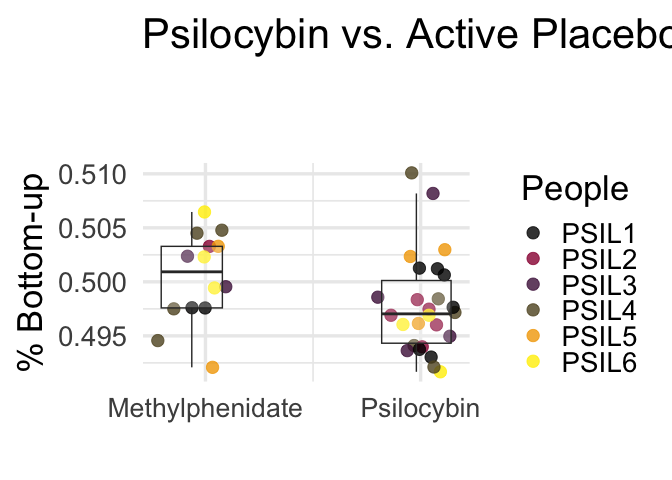
\includegraphics{Stats_n_Viz_files/figure-latex/unnamed-chunk-18-1.pdf}

\begin{Shaded}
\begin{Highlighting}[]
\CommentTok{\# right hemi}
\FunctionTok{ggplot}\NormalTok{(spunR,}\FunctionTok{aes}\NormalTok{(}\AttributeTok{x=}\NormalTok{Var1))}\SpecialCharTok{+}\FunctionTok{geom\_density}\NormalTok{(}\AttributeTok{size=}\FloatTok{1.5}\NormalTok{)}\SpecialCharTok{+}\FunctionTok{geom\_vline}\NormalTok{(}\AttributeTok{xintercept =}\NormalTok{ ObsR}\SpecialCharTok{$}\NormalTok{Var1,}\AttributeTok{size=}\DecValTok{2}\NormalTok{,}\AttributeTok{color=}\StringTok{\textquotesingle{}\#BC3754\textquotesingle{}}\NormalTok{)}\SpecialCharTok{+}\FunctionTok{theme\_classic}\NormalTok{(}\AttributeTok{base\_size=}\DecValTok{23}\NormalTok{)}\SpecialCharTok{+}\FunctionTok{ylab}\NormalTok{(}\StringTok{\textquotesingle{}\textquotesingle{}}\NormalTok{)}\SpecialCharTok{+}\FunctionTok{xlab}\NormalTok{(}\StringTok{\textquotesingle{}T{-}Statistics\textquotesingle{}}\NormalTok{)}\SpecialCharTok{+}\FunctionTok{guides}\NormalTok{(}\AttributeTok{y=}\StringTok{"none"}\NormalTok{)}\SpecialCharTok{+}\FunctionTok{theme}\NormalTok{(}\AttributeTok{axis.text =} \FunctionTok{element\_text}\NormalTok{(}\AttributeTok{size=}\DecValTok{22}\NormalTok{))}\SpecialCharTok{+}\FunctionTok{ggtitle}\NormalTok{(}\StringTok{\textquotesingle{}DMN localization to Yeo7 Boundary: Right hemisphere\textquotesingle{}}\NormalTok{)}
\end{Highlighting}
\end{Shaded}

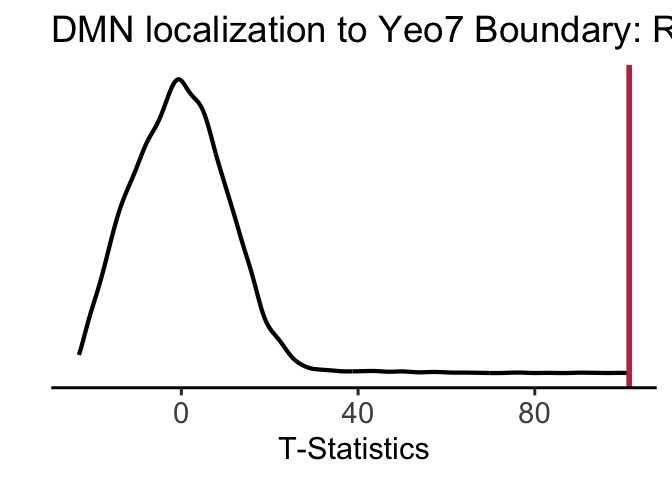
\includegraphics{Stats_n_Viz_files/figure-latex/unnamed-chunk-18-2.pdf}

\begin{Shaded}
\begin{Highlighting}[]
\CommentTok{\# now for biol psych rois}
\NormalTok{bpalign\_L}\OtherTok{=}\FunctionTok{read.csv}\NormalTok{(}\StringTok{\textquotesingle{}\textasciitilde{}/Downloads/perm\_vs\_obs\_DMN\_BiolPsych\_L.csv\textquotesingle{}}\NormalTok{)}
\NormalTok{bpalign\_R}\OtherTok{=}\FunctionTok{read.csv}\NormalTok{(}\StringTok{\textquotesingle{}\textasciitilde{}/Downloads/perm\_vs\_obs\_DMN\_BiolPsych\_R.csv\textquotesingle{}}\NormalTok{)}
\CommentTok{\# add a real vs. permuted value}
\NormalTok{bpalign\_L}\SpecialCharTok{$}\NormalTok{Observed}\OtherTok{=}\DecValTok{0}
\NormalTok{bpalign\_R}\SpecialCharTok{$}\NormalTok{Observed}\OtherTok{=}\DecValTok{0}
\NormalTok{bpalign\_L}\SpecialCharTok{$}\NormalTok{Observed[}\DecValTok{10001}\NormalTok{]}\OtherTok{=}\DecValTok{1}
\NormalTok{bpalign\_R}\SpecialCharTok{$}\NormalTok{Observed[}\DecValTok{10001}\NormalTok{]}\OtherTok{=}\DecValTok{1}
\CommentTok{\# add right vs. left}
\NormalTok{bpalign\_L}\SpecialCharTok{$}\NormalTok{Side}\OtherTok{=}\StringTok{\textquotesingle{}Left\textquotesingle{}}
\NormalTok{bpalign\_R}\SpecialCharTok{$}\NormalTok{Side}\OtherTok{=}\StringTok{\textquotesingle{}Right\textquotesingle{}}

\CommentTok{\# subset spun and nonspun df}
\NormalTok{spunL}\OtherTok{=}\NormalTok{bpalign\_L[}\DecValTok{1}\SpecialCharTok{:}\DecValTok{10000}\NormalTok{,]}
\NormalTok{ObsL}\OtherTok{=}\NormalTok{bpalign\_L[}\DecValTok{10001}\NormalTok{,]}
\NormalTok{spunR}\OtherTok{=}\NormalTok{bpalign\_R[}\DecValTok{1}\SpecialCharTok{:}\DecValTok{10000}\NormalTok{,]}
\NormalTok{ObsR}\OtherTok{=}\NormalTok{bpalign\_R[}\DecValTok{10001}\NormalTok{,]}
  
\CommentTok{\# left hemi}
\FunctionTok{ggplot}\NormalTok{(spunL,}\FunctionTok{aes}\NormalTok{(}\AttributeTok{x=}\NormalTok{Var1))}\SpecialCharTok{+}\FunctionTok{geom\_density}\NormalTok{(}\AttributeTok{size=}\FloatTok{1.5}\NormalTok{)}\SpecialCharTok{+}\FunctionTok{geom\_vline}\NormalTok{(}\AttributeTok{xintercept =}\NormalTok{ ObsL}\SpecialCharTok{$}\NormalTok{Var1,}\AttributeTok{size=}\DecValTok{2}\NormalTok{,}\AttributeTok{color=}\StringTok{\textquotesingle{}\#BC3754\textquotesingle{}}\NormalTok{)}\SpecialCharTok{+}\FunctionTok{theme\_classic}\NormalTok{(}\AttributeTok{base\_size=}\DecValTok{23}\NormalTok{)}\SpecialCharTok{+}\FunctionTok{ylab}\NormalTok{(}\StringTok{\textquotesingle{}\textquotesingle{}}\NormalTok{)}\SpecialCharTok{+}\FunctionTok{xlab}\NormalTok{(}\StringTok{\textquotesingle{}T{-}Statistics\textquotesingle{}}\NormalTok{)}\SpecialCharTok{+}\FunctionTok{guides}\NormalTok{(}\AttributeTok{y=}\StringTok{"none"}\NormalTok{)}\SpecialCharTok{+}\FunctionTok{theme}\NormalTok{(}\AttributeTok{axis.text =} \FunctionTok{element\_text}\NormalTok{(}\AttributeTok{size=}\DecValTok{22}\NormalTok{))}\SpecialCharTok{+}\FunctionTok{ggtitle}\NormalTok{(}\StringTok{\textquotesingle{}DMN localization to Biol. Psych. ROIs: Left hemisphere\textquotesingle{}}\NormalTok{)}
\end{Highlighting}
\end{Shaded}

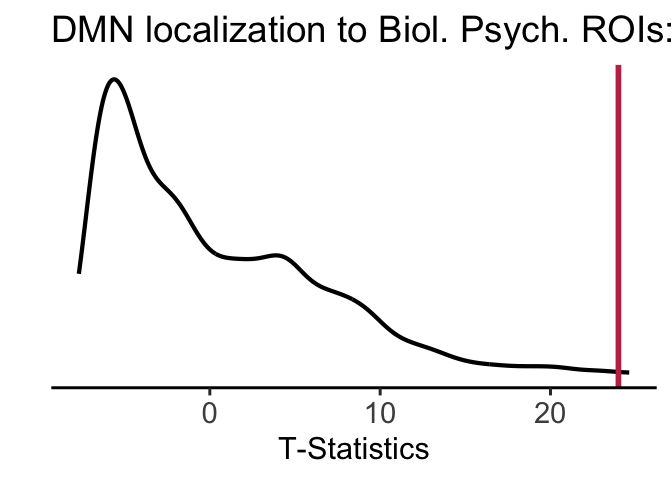
\includegraphics{Stats_n_Viz_files/figure-latex/unnamed-chunk-18-3.pdf}

\begin{Shaded}
\begin{Highlighting}[]
\CommentTok{\# right hemi}
\FunctionTok{ggplot}\NormalTok{(spunR,}\FunctionTok{aes}\NormalTok{(}\AttributeTok{x=}\NormalTok{Var1))}\SpecialCharTok{+}\FunctionTok{geom\_density}\NormalTok{(}\AttributeTok{size=}\FloatTok{1.5}\NormalTok{)}\SpecialCharTok{+}\FunctionTok{geom\_vline}\NormalTok{(}\AttributeTok{xintercept =}\NormalTok{ ObsR}\SpecialCharTok{$}\NormalTok{Var1,}\AttributeTok{size=}\DecValTok{2}\NormalTok{,}\AttributeTok{color=}\StringTok{\textquotesingle{}\#BC3754\textquotesingle{}}\NormalTok{)}\SpecialCharTok{+}\FunctionTok{theme\_classic}\NormalTok{(}\AttributeTok{base\_size=}\DecValTok{23}\NormalTok{)}\SpecialCharTok{+}\FunctionTok{ylab}\NormalTok{(}\StringTok{\textquotesingle{}\textquotesingle{}}\NormalTok{)}\SpecialCharTok{+}\FunctionTok{xlab}\NormalTok{(}\StringTok{\textquotesingle{}T{-}Statistics\textquotesingle{}}\NormalTok{)}\SpecialCharTok{+}\FunctionTok{guides}\NormalTok{(}\AttributeTok{y=}\StringTok{"none"}\NormalTok{)}\SpecialCharTok{+}\FunctionTok{theme}\NormalTok{(}\AttributeTok{axis.text =} \FunctionTok{element\_text}\NormalTok{(}\AttributeTok{size=}\DecValTok{22}\NormalTok{))}\SpecialCharTok{+}\FunctionTok{ggtitle}\NormalTok{(}\StringTok{\textquotesingle{}DMN localization to Biol. Psych. ROIs: Right hemisphere\textquotesingle{}}\NormalTok{)}
\end{Highlighting}
\end{Shaded}

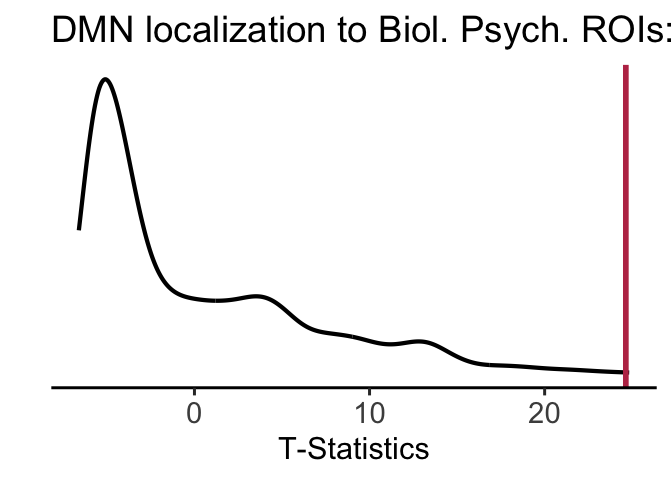
\includegraphics{Stats_n_Viz_files/figure-latex/unnamed-chunk-18-4.pdf}

\begin{Shaded}
\begin{Highlighting}[]
\CommentTok{\# calculate change in DAS to investigate inter{-}psychedelic{-}session variability}
\CommentTok{\# initialize change columns}
\NormalTok{DAS\_Change\_Subject}\OtherTok{=}\FunctionTok{c}\NormalTok{(}\StringTok{\textquotesingle{}\textquotesingle{}}\NormalTok{)}
\NormalTok{DAS\_Change\_Dosage}\OtherTok{=}\FunctionTok{c}\NormalTok{(}\StringTok{\textquotesingle{}\textquotesingle{}}\NormalTok{)}
\NormalTok{DAS\_Change\_ChangeTA}\OtherTok{=}\DecValTok{0}
\NormalTok{DAS\_Change\_ChangeFC}\OtherTok{=}\DecValTok{0}
\NormalTok{DAS\_Change\_ChangeBUP}\OtherTok{=}\DecValTok{0}
\NormalTok{DAS\_Change\_ChangeMag}\OtherTok{=}\DecValTok{0}

\CommentTok{\# isolate drug sessions}
\NormalTok{VASmerge\_DrugSeshs}\OtherTok{=}\NormalTok{VASmerge[VASmerge}\SpecialCharTok{$}\NormalTok{Drug}\SpecialCharTok{==}\DecValTok{1}\NormalTok{,]}
\NormalTok{VASmerge\_Plac}\OtherTok{=}\NormalTok{VASmerge[VASmerge}\SpecialCharTok{$}\NormalTok{Drug}\SpecialCharTok{==}\DecValTok{0}\NormalTok{,]}
\NormalTok{eachSubj}\OtherTok{=}\FunctionTok{unique}\NormalTok{(VASmerge}\SpecialCharTok{$}\NormalTok{Subjects)}

\CommentTok{\# create change from placebo column}
\ControlFlowTok{for}\NormalTok{ (i }\ControlFlowTok{in} \DecValTok{1}\SpecialCharTok{:}\FunctionTok{length}\NormalTok{(eachSubj))\{}
  \CommentTok{\# extract drug sessions}
\NormalTok{  SubjDrug}\OtherTok{=}\NormalTok{VASmerge\_DrugSeshs[VASmerge\_DrugSeshs}\SpecialCharTok{$}\NormalTok{Subjects}\SpecialCharTok{==}\NormalTok{eachSubj[i],]}
\NormalTok{  Subj80}\OtherTok{=}\NormalTok{SubjDrug[SubjDrug}\SpecialCharTok{$}\NormalTok{Dosage}\SpecialCharTok{==}\StringTok{\textquotesingle{}80mg\textquotesingle{}}\NormalTok{,]}
\NormalTok{  Subj120}\OtherTok{=}\NormalTok{SubjDrug[SubjDrug}\SpecialCharTok{$}\NormalTok{Dosage}\SpecialCharTok{==}\StringTok{\textquotesingle{}120mg\textquotesingle{}}\NormalTok{,]}
  \CommentTok{\# extract placebo session}
\NormalTok{  SubjPlac}\OtherTok{=}\NormalTok{VASmerge\_Plac[VASmerge\_Plac}\SpecialCharTok{$}\NormalTok{Subjects}\SpecialCharTok{==}\NormalTok{eachSubj[i],]}

  \CommentTok{\# calculate mean change across scans (TA)}
\NormalTok{  TA\_Plac}\OtherTok{=}\FunctionTok{mean}\NormalTok{(SubjPlac}\SpecialCharTok{$}\NormalTok{AutoCor)}
\NormalTok{  TA\_80}\OtherTok{=}\FunctionTok{mean}\NormalTok{(Subj80}\SpecialCharTok{$}\NormalTok{AutoCor)}
\NormalTok{  TA\_120}\OtherTok{=}\FunctionTok{mean}\NormalTok{(Subj120}\SpecialCharTok{$}\NormalTok{AutoCor)}
\NormalTok{  SubjChange\_TA\_80}\OtherTok{=}\NormalTok{TA\_Plac}\SpecialCharTok{{-}}\NormalTok{TA\_80}
\NormalTok{  SubjChange\_TA\_120}\OtherTok{=}\NormalTok{TA\_Plac}\SpecialCharTok{{-}}\NormalTok{TA\_120}
  
  \CommentTok{\# calculate mean change across scans (DMN integration)}
\NormalTok{  FC\_Plac}\OtherTok{=}\FunctionTok{mean}\NormalTok{(SubjPlac}\SpecialCharTok{$}\NormalTok{DMNFC)}
\NormalTok{  FC\_80}\OtherTok{=}\FunctionTok{mean}\NormalTok{(Subj80}\SpecialCharTok{$}\NormalTok{DMNFC)}
\NormalTok{  FC\_120}\OtherTok{=}\FunctionTok{mean}\NormalTok{(Subj120}\SpecialCharTok{$}\NormalTok{DMNFC)}
\NormalTok{  SubjChange\_FC\_80}\OtherTok{=}\NormalTok{FC\_Plac}\SpecialCharTok{{-}}\NormalTok{FC\_80}
\NormalTok{  SubjChange\_FC\_120}\OtherTok{=}\NormalTok{FC\_Plac}\SpecialCharTok{{-}}\NormalTok{FC\_120}
  
  \CommentTok{\# calculate mean change across scans (BUP)}
\NormalTok{  BUP\_Plac}\OtherTok{=}\FunctionTok{mean}\NormalTok{(SubjPlac}\SpecialCharTok{$}\NormalTok{TDProp1)}
\NormalTok{  BUP\_80}\OtherTok{=}\FunctionTok{mean}\NormalTok{(Subj80}\SpecialCharTok{$}\NormalTok{TDProp1)}
\NormalTok{  BUP\_120}\OtherTok{=}\FunctionTok{mean}\NormalTok{(Subj120}\SpecialCharTok{$}\NormalTok{TDProp1)}
\NormalTok{  SubjChange\_BUP\_80}\OtherTok{=}\NormalTok{BUP\_Plac}\SpecialCharTok{{-}}\NormalTok{BUP\_80}
\NormalTok{  SubjChange\_BUP\_120}\OtherTok{=}\NormalTok{BUP\_Plac}\SpecialCharTok{{-}}\NormalTok{BUP\_120}
  
  \CommentTok{\# calculate mean change across scans (Magnitude)}
\NormalTok{  Mag\_Plac}\OtherTok{=}\FunctionTok{mean}\NormalTok{(SubjPlac}\SpecialCharTok{$}\NormalTok{DMNMag)}
\NormalTok{  Mag\_80}\OtherTok{=}\FunctionTok{mean}\NormalTok{(Subj80}\SpecialCharTok{$}\NormalTok{DMNMag)}
\NormalTok{  Mag\_120}\OtherTok{=}\FunctionTok{mean}\NormalTok{(Subj120}\SpecialCharTok{$}\NormalTok{DMNMag)}
\NormalTok{  SubjChange\_Mag\_80}\OtherTok{=}\NormalTok{Mag\_Plac}\SpecialCharTok{{-}}\NormalTok{Mag\_80}
\NormalTok{  SubjChange\_Mag\_120}\OtherTok{=}\NormalTok{Mag\_Plac}\SpecialCharTok{{-}}\NormalTok{Mag\_120}
  
  \CommentTok{\# put into VAS\_change, 80mg}
\NormalTok{  DAS\_Change\_Subject}\OtherTok{\textless{}{-}}\FunctionTok{c}\NormalTok{(DAS\_Change\_Subject,eachSubj[i])}
\NormalTok{  DAS\_Change\_Dosage}\OtherTok{\textless{}{-}}\FunctionTok{c}\NormalTok{(DAS\_Change\_Dosage,}\StringTok{\textquotesingle{}80mg\textquotesingle{}}\NormalTok{)}
\NormalTok{  DAS\_Change\_ChangeFC}\OtherTok{\textless{}{-}}\FunctionTok{c}\NormalTok{(DAS\_Change\_ChangeFC,SubjChange\_TA\_80)}
\NormalTok{  DAS\_Change\_ChangeTA}\OtherTok{\textless{}{-}}\FunctionTok{c}\NormalTok{(DAS\_Change\_ChangeTA,SubjChange\_FC\_80)}
\NormalTok{  DAS\_Change\_ChangeBUP}\OtherTok{\textless{}{-}}\FunctionTok{c}\NormalTok{(DAS\_Change\_ChangeBUP,SubjChange\_BUP\_80)}
\NormalTok{  DAS\_Change\_ChangeMag}\OtherTok{\textless{}{-}}\FunctionTok{c}\NormalTok{(DAS\_Change\_ChangeMag,SubjChange\_Mag\_80)}
  \CommentTok{\# 120}
\NormalTok{  DAS\_Change\_Subject}\OtherTok{\textless{}{-}}\FunctionTok{c}\NormalTok{(DAS\_Change\_Subject,eachSubj[i])}
\NormalTok{  DAS\_Change\_Dosage}\OtherTok{\textless{}{-}}\FunctionTok{c}\NormalTok{(DAS\_Change\_Dosage,}\StringTok{\textquotesingle{}120mg\textquotesingle{}}\NormalTok{)}
\NormalTok{  DAS\_Change\_ChangeFC}\OtherTok{\textless{}{-}}\FunctionTok{c}\NormalTok{(DAS\_Change\_ChangeFC,SubjChange\_TA\_120)}
\NormalTok{  DAS\_Change\_ChangeTA}\OtherTok{\textless{}{-}}\FunctionTok{c}\NormalTok{(DAS\_Change\_ChangeTA,SubjChange\_FC\_120)}
\NormalTok{  DAS\_Change\_ChangeBUP}\OtherTok{\textless{}{-}}\FunctionTok{c}\NormalTok{(DAS\_Change\_ChangeBUP,SubjChange\_BUP\_120)}
\NormalTok{  DAS\_Change\_ChangeMag}\OtherTok{\textless{}{-}}\FunctionTok{c}\NormalTok{(DAS\_Change\_ChangeMag,SubjChange\_Mag\_120)}
\NormalTok{\}}

\NormalTok{DAS\_changeDF}\OtherTok{=}\FunctionTok{data.frame}\NormalTok{(DAS\_Change\_Subject,DAS\_Change\_Dosage,DAS\_Change\_ChangeFC,DAS\_Change\_ChangeTA,DAS\_Change\_ChangeBUP,DAS\_Change\_ChangeMag)}
\CommentTok{\# drop first row (initialization row)}
\NormalTok{DAS\_changeDF}\OtherTok{=}\NormalTok{DAS\_changeDF[}\SpecialCharTok{{-}}\FunctionTok{c}\NormalTok{(}\DecValTok{1}\NormalTok{),]}
\FunctionTok{colnames}\NormalTok{(DAS\_changeDF)}\OtherTok{\textless{}{-}}\FunctionTok{c}\NormalTok{(}\StringTok{\textquotesingle{}Subjects\textquotesingle{}}\NormalTok{,}\StringTok{\textquotesingle{}Dosage\textquotesingle{}}\NormalTok{,}\StringTok{\textquotesingle{}FC\_Decrease\textquotesingle{}}\NormalTok{,}\StringTok{\textquotesingle{}TA\_Decrease\textquotesingle{}}\NormalTok{,}\StringTok{\textquotesingle{}BUP\_Decrease\textquotesingle{}}\NormalTok{,}\StringTok{\textquotesingle{}Mag\_Decrease\textquotesingle{}}\NormalTok{)}
\CommentTok{\# merge with DAS scores}
\NormalTok{DAS\_changeDF}\OtherTok{=}\FunctionTok{merge}\NormalTok{(DAS\_changeDF,vas,}\AttributeTok{by=}\FunctionTok{c}\NormalTok{(}\StringTok{"Subjects"}\NormalTok{,}\StringTok{"Dosage"}\NormalTok{))}
\CommentTok{\# omit NA rows}
\NormalTok{DAS\_changeDF}\OtherTok{=}\NormalTok{DAS\_changeDF[DAS\_changeDF}\SpecialCharTok{$}\NormalTok{FC\_Decrease}\SpecialCharTok{!=}\StringTok{\textquotesingle{}NaN\textquotesingle{}}\NormalTok{,]}



\CommentTok{\# initialize output correlation stats}
\NormalTok{corvec}\OtherTok{=}\ConstantTok{NULL}
\NormalTok{pvec}\OtherTok{=}\ConstantTok{NULL}
\NormalTok{colNameVec}\OtherTok{=}\ConstantTok{NULL}
\NormalTok{counter}\OtherTok{=}\DecValTok{1}
\CommentTok{\# plot change from placebo with reported DAS scores}
\ControlFlowTok{for}\NormalTok{ (i }\ControlFlowTok{in} \DecValTok{41}\SpecialCharTok{:}\DecValTok{57}\NormalTok{)\{}
  \FunctionTok{plot}\NormalTok{(DAS\_changeDF}\SpecialCharTok{$}\NormalTok{BUP\_Decrease,DAS\_changeDF[,i],}\AttributeTok{main=}\FunctionTok{colnames}\NormalTok{(DAS\_changeDF)[i])}
  \CommentTok{\# note das scores are not normally distriuted, even from drug sessions}
\NormalTok{  a}\OtherTok{=}\FunctionTok{cor.test}\NormalTok{(DAS\_changeDF}\SpecialCharTok{$}\NormalTok{BUP\_Decrease,DAS\_changeDF[,i])}
\NormalTok{  corvec[counter]}\OtherTok{=}\NormalTok{a}\SpecialCharTok{$}\NormalTok{estimate}
\NormalTok{  pvec[counter]}\OtherTok{=}\NormalTok{a}\SpecialCharTok{$}\NormalTok{p.value}
\NormalTok{  colNameVec[counter]}\OtherTok{=}\FunctionTok{colnames}\NormalTok{(DAS\_changeDF)[i]}
\NormalTok{  counter}\OtherTok{=}\NormalTok{counter}\SpecialCharTok{+}\DecValTok{1}
\NormalTok{\}}
\end{Highlighting}
\end{Shaded}

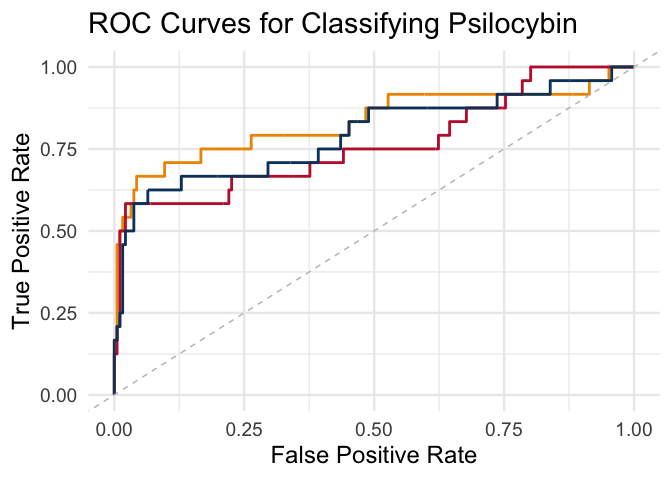
\includegraphics{Stats_n_Viz_files/figure-latex/unnamed-chunk-19-1.pdf}
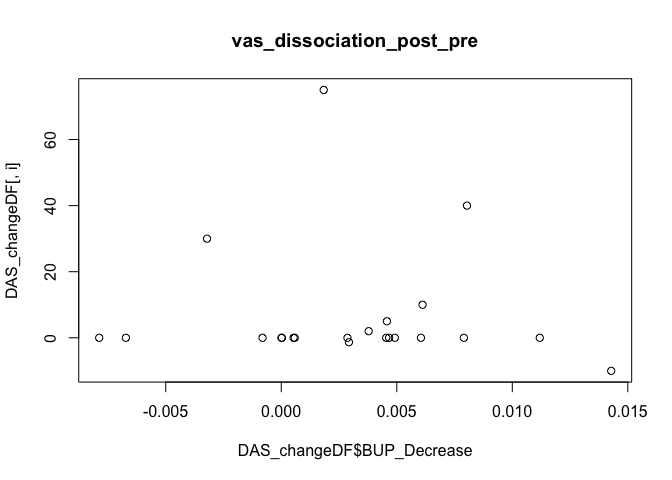
\includegraphics{Stats_n_Viz_files/figure-latex/unnamed-chunk-19-2.pdf}
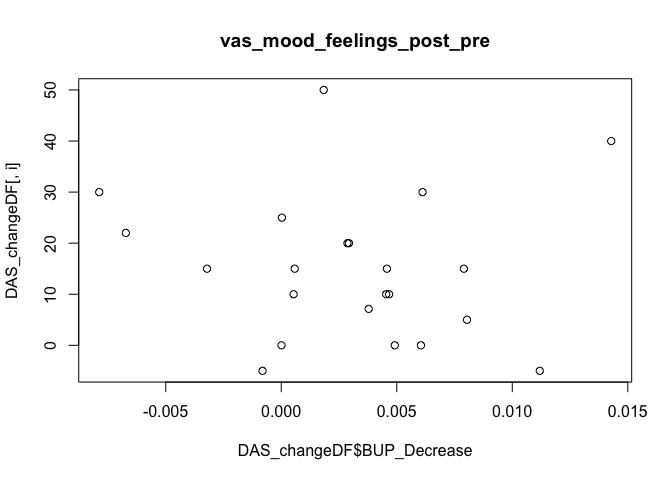
\includegraphics{Stats_n_Viz_files/figure-latex/unnamed-chunk-19-3.pdf}
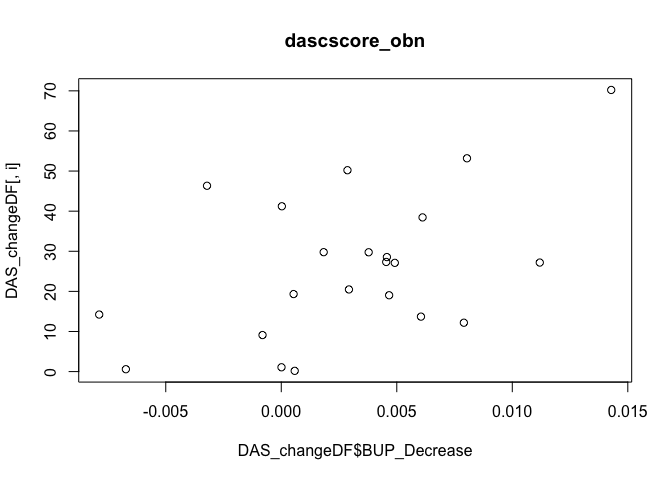
\includegraphics{Stats_n_Viz_files/figure-latex/unnamed-chunk-19-4.pdf}
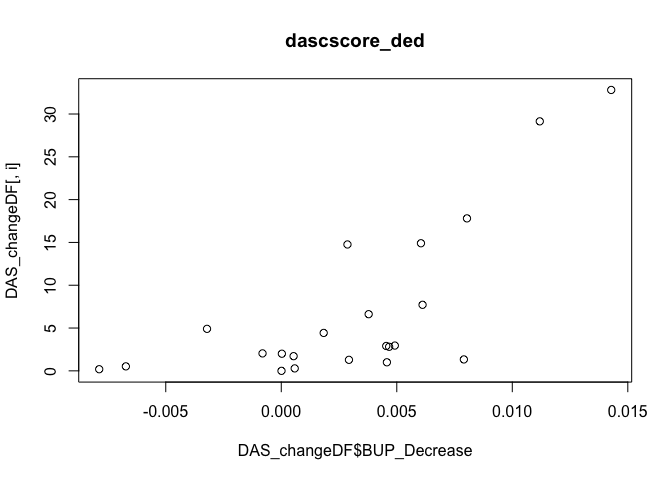
\includegraphics{Stats_n_Viz_files/figure-latex/unnamed-chunk-19-5.pdf}
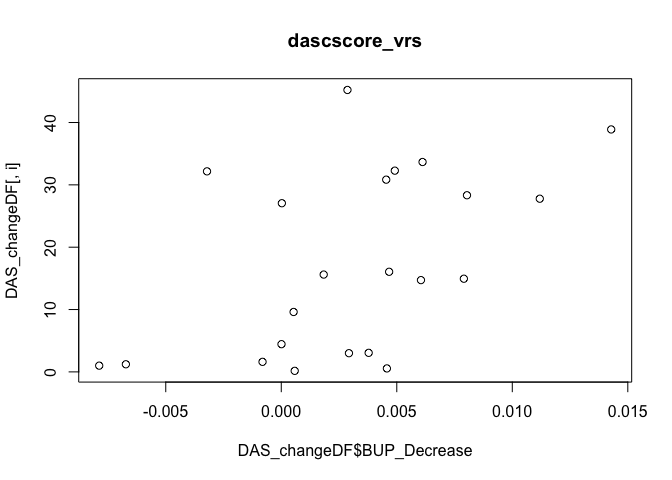
\includegraphics{Stats_n_Viz_files/figure-latex/unnamed-chunk-19-6.pdf}
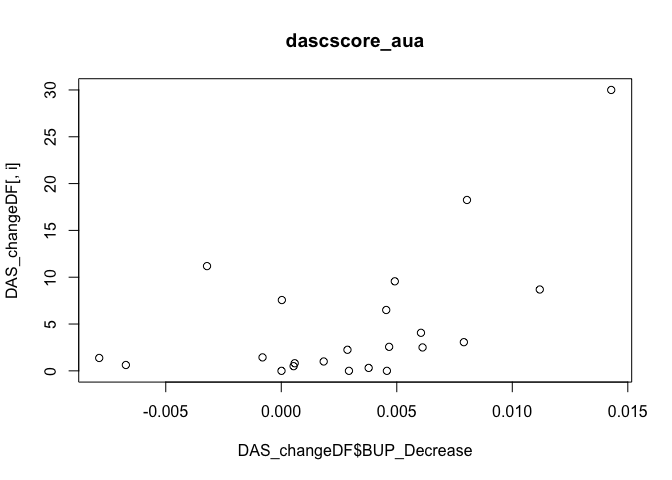
\includegraphics{Stats_n_Viz_files/figure-latex/unnamed-chunk-19-7.pdf}
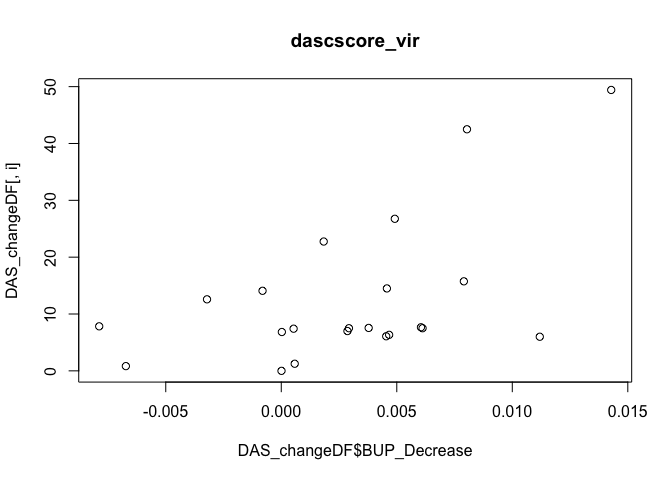
\includegraphics{Stats_n_Viz_files/figure-latex/unnamed-chunk-19-8.pdf}
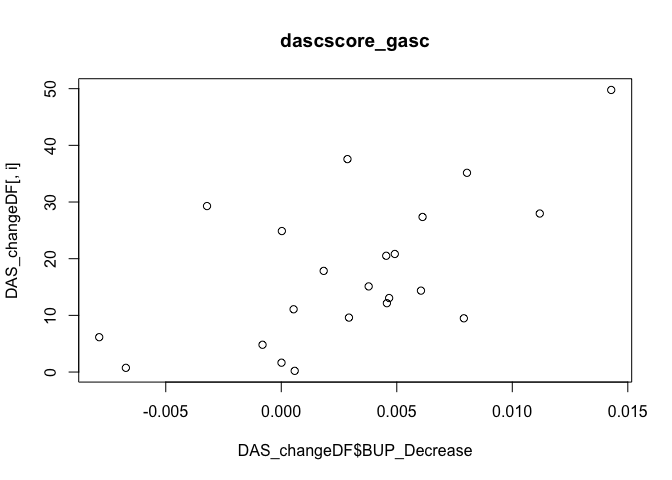
\includegraphics{Stats_n_Viz_files/figure-latex/unnamed-chunk-19-9.pdf}
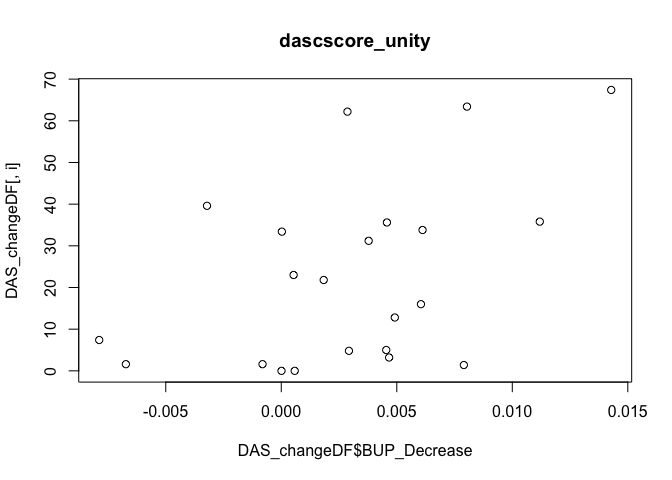
\includegraphics{Stats_n_Viz_files/figure-latex/unnamed-chunk-19-10.pdf}
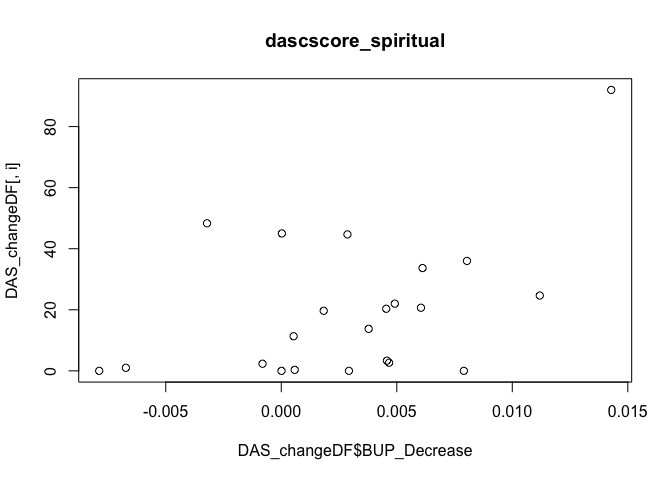
\includegraphics{Stats_n_Viz_files/figure-latex/unnamed-chunk-19-11.pdf}
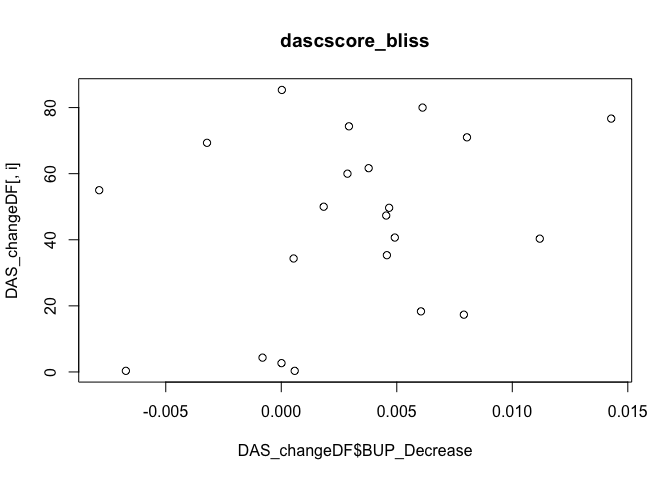
\includegraphics{Stats_n_Viz_files/figure-latex/unnamed-chunk-19-12.pdf}
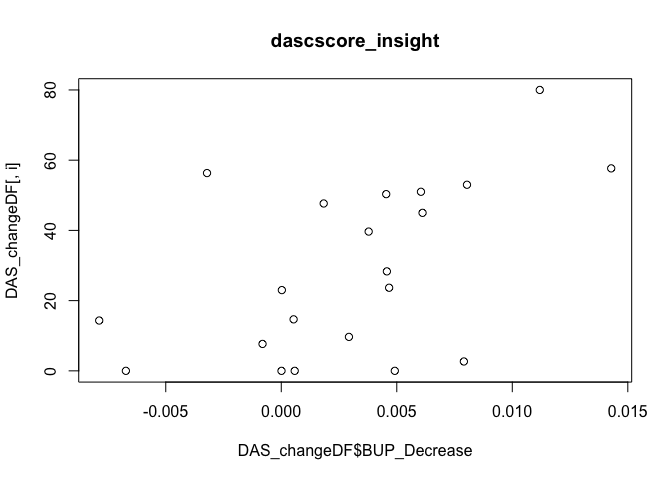
\includegraphics{Stats_n_Viz_files/figure-latex/unnamed-chunk-19-13.pdf}
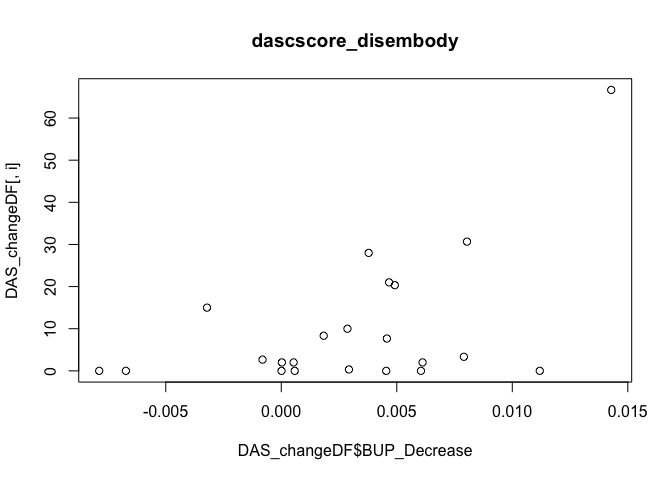
\includegraphics{Stats_n_Viz_files/figure-latex/unnamed-chunk-19-14.pdf}
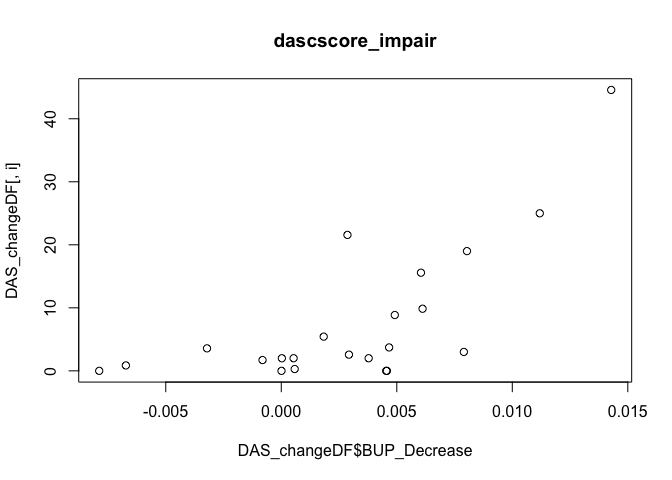
\includegraphics{Stats_n_Viz_files/figure-latex/unnamed-chunk-19-15.pdf}
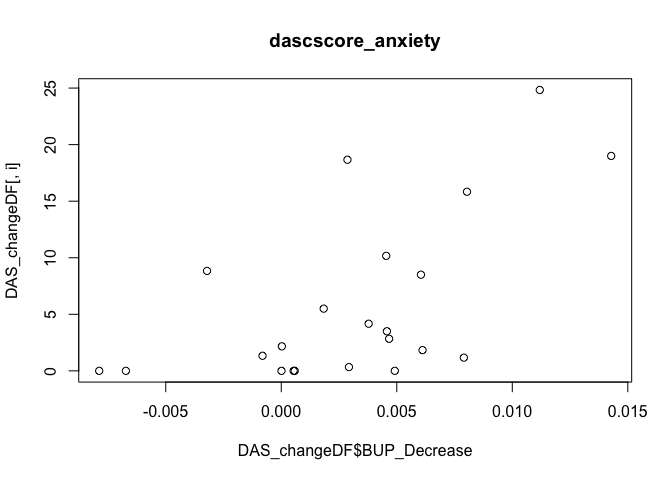
\includegraphics{Stats_n_Viz_files/figure-latex/unnamed-chunk-19-16.pdf}
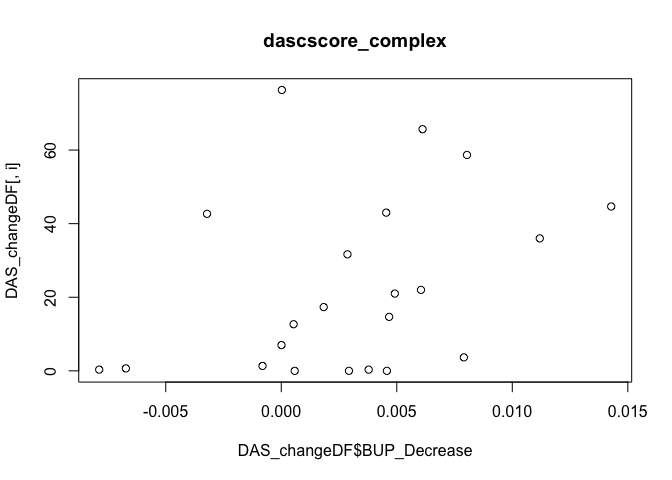
\includegraphics{Stats_n_Viz_files/figure-latex/unnamed-chunk-19-17.pdf}

\begin{Shaded}
\begin{Highlighting}[]
\CommentTok{\# set some colorations to be consistent in new df by subject}
\NormalTok{DAS\_changeDF}\SpecialCharTok{$}\NormalTok{Subjects}\OtherTok{\textless{}{-}}\FunctionTok{as.factor}\NormalTok{(DAS\_changeDF}\SpecialCharTok{$}\NormalTok{Subjects)}
\NormalTok{DAS\_changeDF}\SpecialCharTok{$}\NormalTok{Colors }\OtherTok{\textless{}{-}}\NormalTok{ generated\_colors[DAS\_changeDF}\SpecialCharTok{$}\NormalTok{Subjects]}
\NormalTok{DAS\_changeDF\_people }\OtherTok{\textless{}{-}} \FunctionTok{merge}\NormalTok{(DAS\_changeDF, unique\_pairs, }\AttributeTok{by =} \StringTok{\textquotesingle{}Subjects\textquotesingle{}}\NormalTok{, }\AttributeTok{all.x =} \ConstantTok{TRUE}\NormalTok{)}
\NormalTok{DAS\_changeDF\_people}\SpecialCharTok{$}\NormalTok{SubjectsCols }\OtherTok{\textless{}{-}} \FunctionTok{factor}\NormalTok{(DAS\_changeDF\_people}\SpecialCharTok{$}\NormalTok{Subjects, }\AttributeTok{levels =} \FunctionTok{names}\NormalTok{(generated\_colors))}
\end{Highlighting}
\end{Shaded}

\begin{Shaded}
\begin{Highlighting}[]
\DocumentationTok{\#\#\# figure 3B {-} coarse}
\CommentTok{\# make a vector of DAS scale names \textbackslash{}n is a newline for the ggplots}
\NormalTok{dascNames }\OtherTok{\textless{}{-}} \FunctionTok{c}\NormalTok{(}
  \StringTok{\textquotesingle{}Oceaninc}\SpecialCharTok{\textbackslash{}n}\StringTok{Boundlessness\textquotesingle{}}\NormalTok{,}
  \StringTok{\textquotesingle{}Dread of Ego}\SpecialCharTok{\textbackslash{}n}\StringTok{Dissolution\textquotesingle{}}\NormalTok{,}
  \StringTok{\textquotesingle{}Visionary}\SpecialCharTok{\textbackslash{}n}\StringTok{Restructuralization\textquotesingle{}}\NormalTok{,}
  \StringTok{\textquotesingle{}Auditory}\SpecialCharTok{\textbackslash{}n}\StringTok{Alterations\textquotesingle{}}\NormalTok{,}
  \StringTok{\textquotesingle{}Vigilance}\SpecialCharTok{\textbackslash{}n}\StringTok{Reduction\textquotesingle{}}
\NormalTok{)}

\NormalTok{dascNamesAcr }\OtherTok{\textless{}{-}} \FunctionTok{c}\NormalTok{(}
  \StringTok{\textquotesingle{}O.B.\textquotesingle{}}\NormalTok{,}
  \StringTok{\textquotesingle{}D.E.D.\textquotesingle{}}\NormalTok{,}
  \StringTok{\textquotesingle{}V.Res.\textquotesingle{}}\NormalTok{,}
  \StringTok{\textquotesingle{}A.A.\textquotesingle{}}\NormalTok{,}
  \StringTok{\textquotesingle{}V.Red.\textquotesingle{}}
\NormalTok{)}


\DocumentationTok{\#\#\#\#\# Propagation directions}
\CommentTok{\# initialize correlation vector for dasc}
\NormalTok{BUP\_corvec}\OtherTok{=}\ConstantTok{NULL}
\NormalTok{BUP\_pvec}\OtherTok{=}\ConstantTok{NULL}
\NormalTok{colNameVec}\OtherTok{=}\ConstantTok{NULL}
\CommentTok{\# initialize counter}
\NormalTok{counter}\OtherTok{=}\DecValTok{1}
\ControlFlowTok{for}\NormalTok{ (i }\ControlFlowTok{in} \DecValTok{44}\SpecialCharTok{:}\DecValTok{48}\NormalTok{)\{}
\NormalTok{  a}\OtherTok{=}\FunctionTok{cor.test}\NormalTok{(DAS\_changeDF}\SpecialCharTok{$}\NormalTok{BUP\_Decrease,DAS\_changeDF[,i])}
\NormalTok{  BUP\_corvec[counter] }\OtherTok{\textless{}{-}}\NormalTok{ a}\SpecialCharTok{$}\NormalTok{estimate}
\NormalTok{  BUP\_pvec[counter] }\OtherTok{\textless{}{-}}\NormalTok{ a}\SpecialCharTok{$}\NormalTok{p.value}
\NormalTok{  counter}\OtherTok{=}\NormalTok{counter}\SpecialCharTok{+}\DecValTok{1}
\NormalTok{\}}


\DocumentationTok{\#\#\#\#\#\#\#\#\#}
\CommentTok{\# equivalent for AutoCor}
\DocumentationTok{\#\#\#\#\#\#\#\#\#}

\NormalTok{TA\_corvec}\OtherTok{=}\ConstantTok{NULL}
\NormalTok{TA\_pvec}\OtherTok{=}\ConstantTok{NULL}
\CommentTok{\# initialize counter}
\NormalTok{counter}\OtherTok{=}\DecValTok{1}
\ControlFlowTok{for}\NormalTok{ (i }\ControlFlowTok{in} \DecValTok{44}\SpecialCharTok{:}\DecValTok{48}\NormalTok{)\{}
\NormalTok{  a}\OtherTok{=}\FunctionTok{cor.test}\NormalTok{(DAS\_changeDF}\SpecialCharTok{$}\NormalTok{TA\_Decrease,DAS\_changeDF[,i])}
\NormalTok{  TA\_corvec[counter] }\OtherTok{\textless{}{-}}\NormalTok{ a}\SpecialCharTok{$}\NormalTok{estimate}
\NormalTok{  TA\_pvec[counter] }\OtherTok{\textless{}{-}}\NormalTok{ a}\SpecialCharTok{$}\NormalTok{p.value}
\NormalTok{  counter}\OtherTok{=}\NormalTok{counter}\SpecialCharTok{+}\DecValTok{1}
\NormalTok{\}}


\DocumentationTok{\#\#\#\#\#\#\#\#\#}
\CommentTok{\# equivalent for DMN seg}
\DocumentationTok{\#\#\#\#\#\#\#\#\#}

\NormalTok{S\_corvec}\OtherTok{=}\ConstantTok{NULL}
\NormalTok{S\_pvec}\OtherTok{=}\ConstantTok{NULL}
\CommentTok{\# initialize counter}
\NormalTok{counter}\OtherTok{=}\DecValTok{1}
\ControlFlowTok{for}\NormalTok{ (i }\ControlFlowTok{in} \DecValTok{44}\SpecialCharTok{:}\DecValTok{48}\NormalTok{)\{}
\NormalTok{  a}\OtherTok{=}\FunctionTok{cor.test}\NormalTok{(DAS\_changeDF}\SpecialCharTok{$}\NormalTok{FC\_Decrease,DAS\_changeDF[,i])}
\NormalTok{  S\_corvec[counter] }\OtherTok{\textless{}{-}}\NormalTok{ a}\SpecialCharTok{$}\NormalTok{estimate}
\NormalTok{  S\_pvec[counter] }\OtherTok{\textless{}{-}}\NormalTok{ a}\SpecialCharTok{$}\NormalTok{p.value}
\NormalTok{  counter}\OtherTok{=}\NormalTok{counter}\SpecialCharTok{+}\DecValTok{1}
\NormalTok{\}}

\DocumentationTok{\#\#\#\#\#\#\#\#\#}
\CommentTok{\# equivalent for DMN Magnitude}
\DocumentationTok{\#\#\#\#\#\#\#\#\#}

\NormalTok{M\_corvec}\OtherTok{=}\ConstantTok{NULL}
\NormalTok{M\_pvec}\OtherTok{=}\ConstantTok{NULL}
\CommentTok{\# initialize counter}
\NormalTok{counter}\OtherTok{=}\DecValTok{1}
\ControlFlowTok{for}\NormalTok{ (i }\ControlFlowTok{in} \DecValTok{44}\SpecialCharTok{:}\DecValTok{48}\NormalTok{)\{}
\NormalTok{  a}\OtherTok{=}\FunctionTok{cor.test}\NormalTok{(DAS\_changeDF}\SpecialCharTok{$}\NormalTok{Mag\_Decrease,DAS\_changeDF[,i])}
\NormalTok{  M\_corvec[counter] }\OtherTok{\textless{}{-}}\NormalTok{ a}\SpecialCharTok{$}\NormalTok{estimate}
\NormalTok{  M\_pvec[counter] }\OtherTok{\textless{}{-}}\NormalTok{ a}\SpecialCharTok{$}\NormalTok{p.value}
\NormalTok{  counter}\OtherTok{=}\NormalTok{counter}\SpecialCharTok{+}\DecValTok{1}
\NormalTok{\}}

\CommentTok{\# correct all for multiple comparisons}
\NormalTok{allPs}\OtherTok{=}\FunctionTok{c}\NormalTok{(S\_pvec,TA\_pvec,BUP\_pvec,M\_pvec)}
\NormalTok{allPs\_MC}\OtherTok{=}\FunctionTok{p.adjust}\NormalTok{(allPs,}\AttributeTok{method=}\StringTok{\textquotesingle{}fdr\textquotesingle{}}\NormalTok{)}

\CommentTok{\# pull out S pvecs}
\NormalTok{S\_pvec\_mc}\OtherTok{=}\NormalTok{allPs\_MC[}\DecValTok{1}\SpecialCharTok{:}\DecValTok{5}\NormalTok{]}
\NormalTok{TA\_pvec\_mc}\OtherTok{=}\NormalTok{allPs\_MC[}\DecValTok{6}\SpecialCharTok{:}\DecValTok{10}\NormalTok{]}
\NormalTok{BUP\_pvec\_mc}\OtherTok{=}\NormalTok{allPs\_MC[}\DecValTok{11}\SpecialCharTok{:}\DecValTok{15}\NormalTok{]}
\NormalTok{M\_pvec\_mc}\OtherTok{=}\NormalTok{allPs\_MC[}\DecValTok{16}\SpecialCharTok{:}\DecValTok{20}\NormalTok{]}

\CommentTok{\# BAR PLOTS FOR ALL}
\CommentTok{\# DMN SEGREGATION}
\CommentTok{\# Create a dataframe with the values and column names}
\NormalTok{df }\OtherTok{\textless{}{-}} \FunctionTok{data.frame}\NormalTok{(}\AttributeTok{Values =}\NormalTok{ S\_corvec, }\AttributeTok{pvals=}\NormalTok{S\_pvec)}

\CommentTok{\# make a color vector by significance}
\NormalTok{colorvec}\OtherTok{=}\FunctionTok{rep}\NormalTok{(}\StringTok{\textquotesingle{}NS\textquotesingle{}}\NormalTok{,}\DecValTok{5}\NormalTok{)}
\NormalTok{colorvec[S\_pvec}\SpecialCharTok{\textless{}}\NormalTok{.}\DecValTok{05}\NormalTok{]}\OtherTok{=}\StringTok{\textquotesingle{}Uncr\textquotesingle{}}
\NormalTok{colorvec[S\_pvec\_mc}\SpecialCharTok{\textless{}}\NormalTok{.}\DecValTok{05}\NormalTok{]}\OtherTok{=}\StringTok{\textquotesingle{}FDR\textquotesingle{}}
\NormalTok{df}\SpecialCharTok{$}\NormalTok{Sig }\OtherTok{\textless{}{-}} \FunctionTok{factor}\NormalTok{(colorvec, }\AttributeTok{levels =} \FunctionTok{c}\NormalTok{(}\StringTok{\textquotesingle{}NS\textquotesingle{}}\NormalTok{, }\StringTok{\textquotesingle{}Uncr\textquotesingle{}}\NormalTok{, }\StringTok{\textquotesingle{}FDR\textquotesingle{}}\NormalTok{))}
\CommentTok{\# Specify color scale manually}
\NormalTok{colors }\OtherTok{\textless{}{-}} \FunctionTok{c}\NormalTok{(}\StringTok{\textquotesingle{}NS\textquotesingle{}} \OtherTok{=} \StringTok{\textquotesingle{}\#002642\textquotesingle{}}\NormalTok{, }\StringTok{\textquotesingle{}Uncr\textquotesingle{}} \OtherTok{=} \StringTok{\textquotesingle{}\#EF9500\textquotesingle{}}\NormalTok{, }\StringTok{\textquotesingle{}FDR\textquotesingle{}} \OtherTok{=} \StringTok{\textquotesingle{}\#840032\textquotesingle{}}\NormalTok{)}
\NormalTok{df}\SpecialCharTok{$}\NormalTok{ColumnNamesAcr}\OtherTok{\textless{}{-}}\FunctionTok{c}\NormalTok{(dascNames)}
\CommentTok{\# linear version}
\FunctionTok{ggplot}\NormalTok{(df, }\FunctionTok{aes}\NormalTok{(}\AttributeTok{x =}\NormalTok{ Values, }\AttributeTok{y =}\NormalTok{ dascNames,}\AttributeTok{fill=}\NormalTok{Sig)) }\SpecialCharTok{+}
  \FunctionTok{geom\_bar}\NormalTok{(}\AttributeTok{size=}\DecValTok{3}\NormalTok{,}\AttributeTok{stat =} \StringTok{"identity"}\NormalTok{)}\SpecialCharTok{+}
  \FunctionTok{scale\_fill\_manual}\NormalTok{(}\AttributeTok{values =}\NormalTok{ colors) }\SpecialCharTok{+}
  \FunctionTok{labs}\NormalTok{(}\AttributeTok{y =} \StringTok{""}\NormalTok{, }\AttributeTok{x =} \StringTok{"Subscale Correlation"}\NormalTok{,}\AttributeTok{title=}\StringTok{"Change in Integration"}\NormalTok{)}\SpecialCharTok{+}\FunctionTok{theme\_minimal}\NormalTok{(}\AttributeTok{base\_size=}\DecValTok{17}\NormalTok{)}\SpecialCharTok{+}\FunctionTok{xlim}\NormalTok{(}\FunctionTok{c}\NormalTok{(}\SpecialCharTok{{-}}\NormalTok{.}\DecValTok{3}\NormalTok{,.}\DecValTok{8}\NormalTok{))}\SpecialCharTok{+}
  \FunctionTok{theme}\NormalTok{(}\AttributeTok{legend.position=}\StringTok{\textquotesingle{}none\textquotesingle{}}\NormalTok{)}
\end{Highlighting}
\end{Shaded}

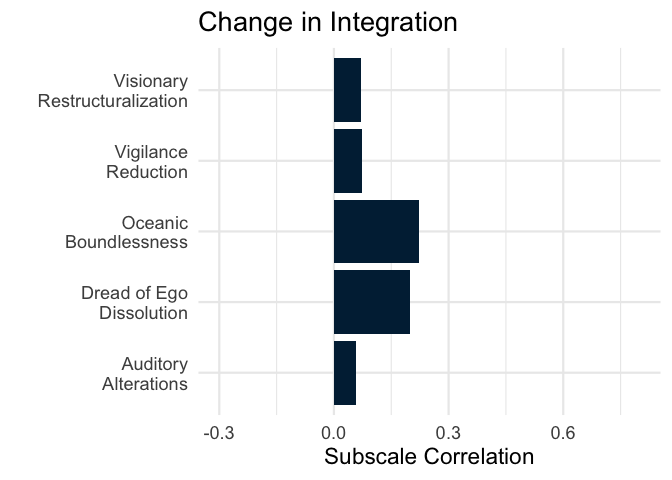
\includegraphics{Stats_n_Viz_files/figure-latex/unnamed-chunk-20-1.pdf}

\begin{Shaded}
\begin{Highlighting}[]
\CommentTok{\# DMN AUTOCOTR}
\CommentTok{\# Create a dataframe with the values and column names}
\NormalTok{df }\OtherTok{\textless{}{-}} \FunctionTok{data.frame}\NormalTok{(}\AttributeTok{Values =}\NormalTok{ TA\_corvec, }\AttributeTok{pvals=}\NormalTok{TA\_pvec)}

\CommentTok{\# make a color vector by significance}
\NormalTok{colorvec}\OtherTok{=}\FunctionTok{rep}\NormalTok{(}\StringTok{\textquotesingle{}NS\textquotesingle{}}\NormalTok{,}\DecValTok{5}\NormalTok{)}
\NormalTok{colorvec[TA\_pvec}\SpecialCharTok{\textless{}}\NormalTok{.}\DecValTok{05}\NormalTok{]}\OtherTok{=}\StringTok{\textquotesingle{}Uncr\textquotesingle{}}
\NormalTok{colorvec[TA\_pvec\_mc}\SpecialCharTok{\textless{}}\NormalTok{.}\DecValTok{05}\NormalTok{]}\OtherTok{=}\StringTok{\textquotesingle{}FDR\textquotesingle{}}
\NormalTok{df}\SpecialCharTok{$}\NormalTok{Sig }\OtherTok{\textless{}{-}} \FunctionTok{factor}\NormalTok{(colorvec, }\AttributeTok{levels =} \FunctionTok{c}\NormalTok{(}\StringTok{\textquotesingle{}NS\textquotesingle{}}\NormalTok{, }\StringTok{\textquotesingle{}Uncr\textquotesingle{}}\NormalTok{, }\StringTok{\textquotesingle{}FDR\textquotesingle{}}\NormalTok{))}
\CommentTok{\# Specify color scale manually}
\NormalTok{colors }\OtherTok{\textless{}{-}} \FunctionTok{c}\NormalTok{(}\StringTok{\textquotesingle{}NS\textquotesingle{}} \OtherTok{=} \StringTok{\textquotesingle{}\#002642\textquotesingle{}}\NormalTok{, }\StringTok{\textquotesingle{}Uncr\textquotesingle{}} \OtherTok{=} \StringTok{\textquotesingle{}\#EF9500\textquotesingle{}}\NormalTok{, }\StringTok{\textquotesingle{}FDR\textquotesingle{}} \OtherTok{=} \StringTok{\textquotesingle{}\#840032\textquotesingle{}}\NormalTok{)}
\NormalTok{df}\SpecialCharTok{$}\NormalTok{ColumnNamesAcr}\OtherTok{\textless{}{-}}\FunctionTok{c}\NormalTok{(dascNamesAcr)}
\CommentTok{\# bar version}
\FunctionTok{ggplot}\NormalTok{(df, }\FunctionTok{aes}\NormalTok{(}\AttributeTok{x =}\NormalTok{ Values, }\AttributeTok{y =}\NormalTok{ ColumnNamesAcr,}\AttributeTok{fill=}\NormalTok{Sig)) }\SpecialCharTok{+}
  \FunctionTok{geom\_bar}\NormalTok{(}\AttributeTok{size=}\DecValTok{3}\NormalTok{,}\AttributeTok{stat =} \StringTok{"identity"}\NormalTok{)}\SpecialCharTok{+}
  \FunctionTok{scale\_fill\_manual}\NormalTok{(}\AttributeTok{values =}\NormalTok{ colors) }\SpecialCharTok{+}
  \FunctionTok{labs}\NormalTok{(}\AttributeTok{y =} \StringTok{""}\NormalTok{, }\AttributeTok{x =} \StringTok{"Subscale Correlation"}\NormalTok{,}\AttributeTok{title=}\StringTok{"Change in Autocorrelation"}\NormalTok{)}\SpecialCharTok{+}\FunctionTok{theme\_minimal}\NormalTok{(}\AttributeTok{base\_size=}\DecValTok{17}\NormalTok{)}\SpecialCharTok{+}\FunctionTok{xlim}\NormalTok{(}\FunctionTok{c}\NormalTok{(}\SpecialCharTok{{-}}\NormalTok{.}\DecValTok{3}\NormalTok{,.}\DecValTok{8}\NormalTok{))}\SpecialCharTok{+}
  \FunctionTok{theme}\NormalTok{(}\AttributeTok{legend.position=}\StringTok{\textquotesingle{}none\textquotesingle{}}\NormalTok{)}
\end{Highlighting}
\end{Shaded}

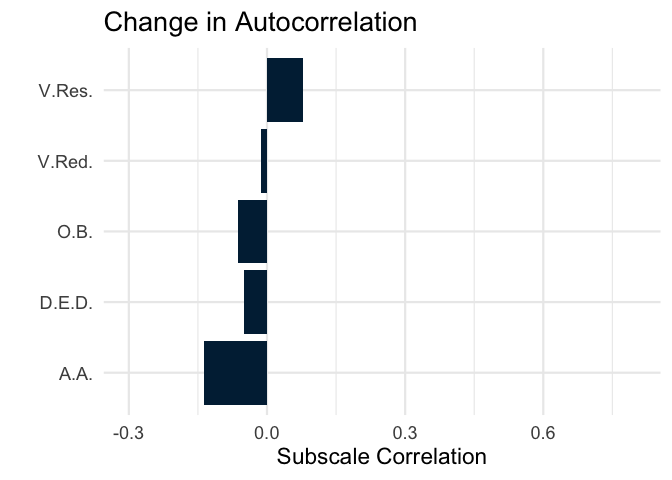
\includegraphics{Stats_n_Viz_files/figure-latex/unnamed-chunk-20-2.pdf}

\begin{Shaded}
\begin{Highlighting}[]
\CommentTok{\# DMN BUP}
\CommentTok{\# Create a dataframe with the values and column names}
\NormalTok{df }\OtherTok{\textless{}{-}} \FunctionTok{data.frame}\NormalTok{(}\AttributeTok{Values =}\NormalTok{ BUP\_corvec, }\AttributeTok{pvals=}\NormalTok{BUP\_pvec)}

\CommentTok{\# make a color vector by significance}
\NormalTok{colorvec}\OtherTok{=}\FunctionTok{rep}\NormalTok{(}\StringTok{\textquotesingle{}NS\textquotesingle{}}\NormalTok{,}\DecValTok{5}\NormalTok{)}
\NormalTok{colorvec[BUP\_pvec}\SpecialCharTok{\textless{}}\NormalTok{.}\DecValTok{05}\NormalTok{]}\OtherTok{=}\StringTok{\textquotesingle{}Uncr\textquotesingle{}}
\NormalTok{colorvec[BUP\_pvec\_mc}\SpecialCharTok{\textless{}}\NormalTok{.}\DecValTok{05}\NormalTok{]}\OtherTok{=}\StringTok{\textquotesingle{}FDR\textquotesingle{}}
\NormalTok{df}\SpecialCharTok{$}\NormalTok{Sig }\OtherTok{\textless{}{-}} \FunctionTok{factor}\NormalTok{(colorvec, }\AttributeTok{levels =} \FunctionTok{c}\NormalTok{(}\StringTok{\textquotesingle{}NS\textquotesingle{}}\NormalTok{, }\StringTok{\textquotesingle{}Uncr\textquotesingle{}}\NormalTok{, }\StringTok{\textquotesingle{}FDR\textquotesingle{}}\NormalTok{))}
\CommentTok{\# Specify color scale manually}
\NormalTok{colors }\OtherTok{\textless{}{-}} \FunctionTok{c}\NormalTok{(}\StringTok{\textquotesingle{}NS\textquotesingle{}} \OtherTok{=} \StringTok{\textquotesingle{}\#002642\textquotesingle{}}\NormalTok{, }\StringTok{\textquotesingle{}Uncr\textquotesingle{}} \OtherTok{=} \StringTok{\textquotesingle{}\#EF9500\textquotesingle{}}\NormalTok{, }\StringTok{\textquotesingle{}FDR\textquotesingle{}} \OtherTok{=} \StringTok{\textquotesingle{}\#840032\textquotesingle{}}\NormalTok{)}
\NormalTok{df}\SpecialCharTok{$}\NormalTok{ColumnNamesAcr}\OtherTok{\textless{}{-}}\FunctionTok{c}\NormalTok{(dascNamesAcr)}
\CommentTok{\# bar version}
\FunctionTok{ggplot}\NormalTok{(df, }\FunctionTok{aes}\NormalTok{(}\AttributeTok{x =}\NormalTok{ Values, }\AttributeTok{y =}\NormalTok{ ColumnNamesAcr,}\AttributeTok{fill=}\NormalTok{Sig)) }\SpecialCharTok{+}
  \FunctionTok{geom\_bar}\NormalTok{(}\AttributeTok{size=}\DecValTok{3}\NormalTok{,}\AttributeTok{stat =} \StringTok{"identity"}\NormalTok{)}\SpecialCharTok{+}
  \FunctionTok{scale\_fill\_manual}\NormalTok{(}\AttributeTok{values =}\NormalTok{ colors) }\SpecialCharTok{+}
  \FunctionTok{labs}\NormalTok{(}\AttributeTok{y =} \StringTok{""}\NormalTok{, }\AttributeTok{x =} \StringTok{"Subscale Correlation"}\NormalTok{,}\AttributeTok{title=}\StringTok{"Change in Prop. Direction"}\NormalTok{)}\SpecialCharTok{+}\FunctionTok{theme\_minimal}\NormalTok{(}\AttributeTok{base\_size=}\DecValTok{17}\NormalTok{)}\SpecialCharTok{+}\FunctionTok{xlim}\NormalTok{(}\FunctionTok{c}\NormalTok{(}\SpecialCharTok{{-}}\NormalTok{.}\DecValTok{3}\NormalTok{,.}\DecValTok{8}\NormalTok{))}\SpecialCharTok{+}
  \FunctionTok{theme}\NormalTok{(}\AttributeTok{legend.position=}\StringTok{\textquotesingle{}none\textquotesingle{}}\NormalTok{)}
\end{Highlighting}
\end{Shaded}

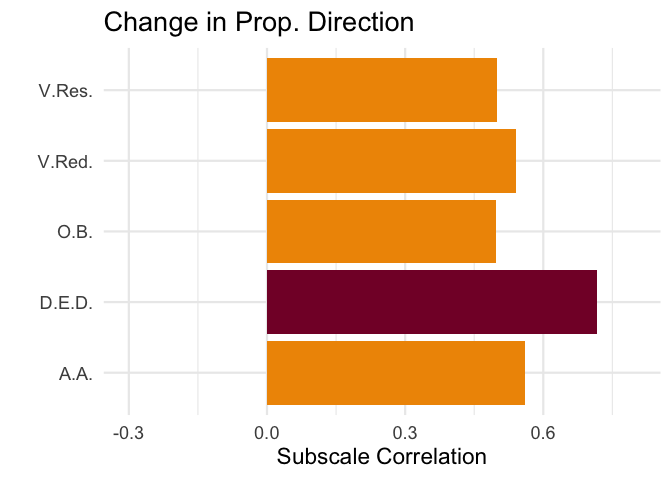
\includegraphics{Stats_n_Viz_files/figure-latex/unnamed-chunk-20-3.pdf}

\begin{Shaded}
\begin{Highlighting}[]
\CommentTok{\# DMN Mag}
\CommentTok{\# Create a dataframe with the values and column names}
\NormalTok{df }\OtherTok{\textless{}{-}} \FunctionTok{data.frame}\NormalTok{(}\AttributeTok{Values =}\NormalTok{ M\_corvec, }\AttributeTok{pvals=}\NormalTok{M\_pvec)}

\CommentTok{\# make a color vector by significance}
\NormalTok{colorvec}\OtherTok{=}\FunctionTok{rep}\NormalTok{(}\StringTok{\textquotesingle{}NS\textquotesingle{}}\NormalTok{,}\DecValTok{5}\NormalTok{)}
\NormalTok{colorvec[M\_pvec}\SpecialCharTok{\textless{}}\NormalTok{.}\DecValTok{05}\NormalTok{]}\OtherTok{=}\StringTok{\textquotesingle{}Uncr\textquotesingle{}}
\NormalTok{colorvec[M\_pvec\_mc}\SpecialCharTok{\textless{}}\NormalTok{.}\DecValTok{05}\NormalTok{]}\OtherTok{=}\StringTok{\textquotesingle{}FDR\textquotesingle{}}
\NormalTok{df}\SpecialCharTok{$}\NormalTok{Sig }\OtherTok{\textless{}{-}} \FunctionTok{factor}\NormalTok{(colorvec, }\AttributeTok{levels =} \FunctionTok{c}\NormalTok{(}\StringTok{\textquotesingle{}NS\textquotesingle{}}\NormalTok{, }\StringTok{\textquotesingle{}Uncr\textquotesingle{}}\NormalTok{, }\StringTok{\textquotesingle{}FDR\textquotesingle{}}\NormalTok{))}
\CommentTok{\# Specify color scale manually}
\NormalTok{colors }\OtherTok{\textless{}{-}} \FunctionTok{c}\NormalTok{(}\StringTok{\textquotesingle{}NS\textquotesingle{}} \OtherTok{=} \StringTok{\textquotesingle{}\#002642\textquotesingle{}}\NormalTok{, }\StringTok{\textquotesingle{}Uncr\textquotesingle{}} \OtherTok{=} \StringTok{\textquotesingle{}\#EF9500\textquotesingle{}}\NormalTok{, }\StringTok{\textquotesingle{}FDR\textquotesingle{}} \OtherTok{=} \StringTok{\textquotesingle{}\#840032\textquotesingle{}}\NormalTok{)}
\NormalTok{df}\SpecialCharTok{$}\NormalTok{ColumnNamesAcr}\OtherTok{\textless{}{-}}\FunctionTok{c}\NormalTok{(dascNamesAcr)}
\CommentTok{\# bar version}
\FunctionTok{ggplot}\NormalTok{(df, }\FunctionTok{aes}\NormalTok{(}\AttributeTok{x =}\NormalTok{ Values, }\AttributeTok{y =}\NormalTok{ ColumnNamesAcr,}\AttributeTok{fill=}\NormalTok{Sig)) }\SpecialCharTok{+}
  \FunctionTok{geom\_bar}\NormalTok{(}\AttributeTok{size=}\DecValTok{3}\NormalTok{,}\AttributeTok{stat =} \StringTok{"identity"}\NormalTok{)}\SpecialCharTok{+}
  \FunctionTok{scale\_fill\_manual}\NormalTok{(}\AttributeTok{values =}\NormalTok{ colors) }\SpecialCharTok{+}
  \FunctionTok{labs}\NormalTok{(}\AttributeTok{y =} \StringTok{""}\NormalTok{, }\AttributeTok{x =} \StringTok{"Subscale Correlation"}\NormalTok{,}\AttributeTok{title=}\StringTok{"Change in Prop. Magnitudes"}\NormalTok{)}\SpecialCharTok{+}\FunctionTok{theme\_minimal}\NormalTok{(}\AttributeTok{base\_size=}\DecValTok{17}\NormalTok{)}\SpecialCharTok{+}\FunctionTok{xlim}\NormalTok{(}\FunctionTok{c}\NormalTok{(}\SpecialCharTok{{-}}\NormalTok{.}\DecValTok{4}\NormalTok{,.}\DecValTok{9}\NormalTok{))}\SpecialCharTok{+}
  \FunctionTok{theme}\NormalTok{(}\AttributeTok{legend.position=}\StringTok{\textquotesingle{}none\textquotesingle{}}\NormalTok{)}
\end{Highlighting}
\end{Shaded}

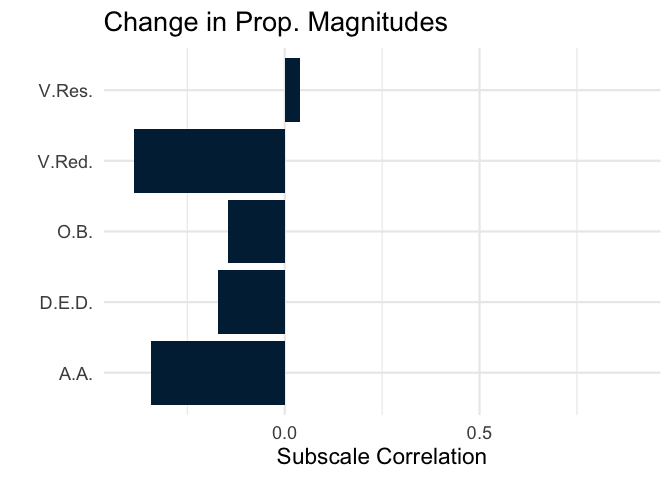
\includegraphics{Stats_n_Viz_files/figure-latex/unnamed-chunk-20-4.pdf}

\begin{Shaded}
\begin{Highlighting}[]
\CommentTok{\# pull out BUP\textasciitilde{}DED correlation}
\FunctionTok{ggplot}\NormalTok{(}\AttributeTok{data=}\NormalTok{DAS\_changeDF\_people,}\FunctionTok{aes}\NormalTok{(}\AttributeTok{y=}\NormalTok{dascscore\_ded,}\AttributeTok{x=}\NormalTok{BUP\_Decrease))}\SpecialCharTok{+}
  \FunctionTok{geom\_point}\NormalTok{(}\AttributeTok{size=}\DecValTok{4}\NormalTok{,}\FunctionTok{aes}\NormalTok{(}\AttributeTok{color =}\NormalTok{ People))}\SpecialCharTok{+}
  \FunctionTok{labs}\NormalTok{(}\AttributeTok{x =} \StringTok{"Decrease in Bottom{-}up \%"}\NormalTok{, }\AttributeTok{y =} \StringTok{"Increase in Dread of Ego Dissolution"}\NormalTok{, }\AttributeTok{color =} \StringTok{"People"}\NormalTok{) }\SpecialCharTok{+}
  \FunctionTok{scale\_color\_manual}\NormalTok{(}\AttributeTok{values =}\NormalTok{ generated\_colors) }\SpecialCharTok{+}
  \FunctionTok{theme\_minimal}\NormalTok{(}\AttributeTok{base\_size =} \DecValTok{16}\NormalTok{)}
\end{Highlighting}
\end{Shaded}

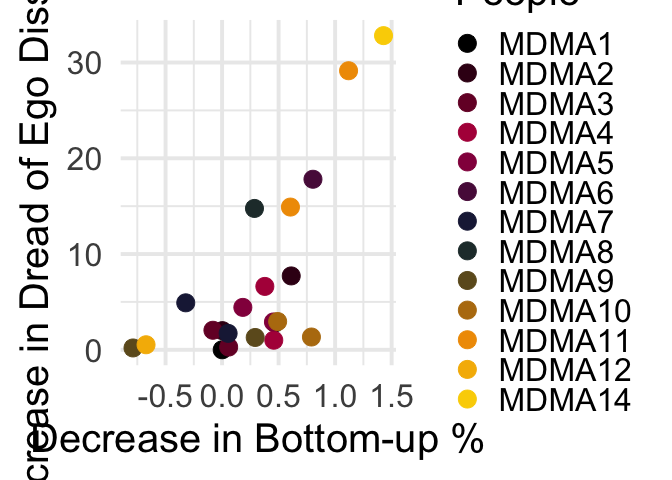
\includegraphics{Stats_n_Viz_files/figure-latex/unnamed-chunk-20-5.pdf}

\begin{Shaded}
\begin{Highlighting}[]
\FunctionTok{cor.test}\NormalTok{(DAS\_changeDF\_people}\SpecialCharTok{$}\NormalTok{dascscore\_ded,DAS\_changeDF\_people}\SpecialCharTok{$}\NormalTok{BUP\_Decrease)}
\end{Highlighting}
\end{Shaded}

\begin{verbatim}
## 
##  Pearson's product-moment correlation
## 
## data:  DAS_changeDF_people$dascscore_ded and DAS_changeDF_people$BUP_Decrease
## t = 4.5982, df = 20, p-value = 0.0001741
## alternative hypothesis: true correlation is not equal to 0
## 95 percent confidence interval:
##  0.4231442 0.8742441
## sample estimates:
##       cor 
## 0.7168634
\end{verbatim}

\begin{Shaded}
\begin{Highlighting}[]
\DocumentationTok{\#\#\# figure 3B {-} granular}
\CommentTok{\# make a vector of DAS scale names \textbackslash{}n is a newline for the ggplots}
\NormalTok{dascNames}\OtherTok{=}\FunctionTok{c}\NormalTok{(}\StringTok{\textquotesingle{}Experience of Unity\textquotesingle{}}\NormalTok{,}\StringTok{\textquotesingle{}Spirtual Experience\textquotesingle{}}\NormalTok{,}\StringTok{\textquotesingle{}Blissful State\textquotesingle{}}\NormalTok{,}\StringTok{\textquotesingle{}Insightfulness\textquotesingle{}}\NormalTok{,}\StringTok{\textquotesingle{}Disembodiment\textquotesingle{}}\NormalTok{,}\StringTok{\textquotesingle{}Impaired Control\textquotesingle{}}\NormalTok{,}\StringTok{\textquotesingle{}Anxiety\textquotesingle{}}\NormalTok{,}\StringTok{\textquotesingle{}Complex Imagery\textquotesingle{}}\NormalTok{,}\StringTok{\textquotesingle{}Elementary Imagery\textquotesingle{}}\NormalTok{,}\StringTok{\textquotesingle{}Synsthesia\textquotesingle{}}\NormalTok{,}\StringTok{\textquotesingle{}Changed meaning}\SpecialCharTok{\textbackslash{}n}\StringTok{ of precepts\textquotesingle{}}\NormalTok{)}

\NormalTok{dascNamesAcr }\OtherTok{\textless{}{-}} \FunctionTok{c}\NormalTok{(}
  \StringTok{\textquotesingle{}E.U.\textquotesingle{}}\NormalTok{,}
  \StringTok{\textquotesingle{}S.E.\textquotesingle{}}\NormalTok{,}
  \StringTok{\textquotesingle{}B.S.\textquotesingle{}}\NormalTok{,}
  \StringTok{\textquotesingle{}Ins.\textquotesingle{}}\NormalTok{,}
  \StringTok{\textquotesingle{}Disemb.\textquotesingle{}}\NormalTok{,}
  \StringTok{\textquotesingle{}I.C.\textquotesingle{}}\NormalTok{,}
  \StringTok{\textquotesingle{}Anx.\textquotesingle{}}\NormalTok{,}
  \StringTok{\textquotesingle{}C.Im.\textquotesingle{}}\NormalTok{,}
  \StringTok{\textquotesingle{}E.Im.\textquotesingle{}}\NormalTok{,}
  \StringTok{\textquotesingle{}Syn.\textquotesingle{}}\NormalTok{,}
  \StringTok{\textquotesingle{}C.M.O.P.\textquotesingle{}}
\NormalTok{)}
\DocumentationTok{\#\#\#\#\# Propagation directions}
\CommentTok{\# initialize correlation vector for dasc}
\NormalTok{BUP\_corvec}\OtherTok{=}\ConstantTok{NULL}
\NormalTok{BUP\_pvec}\OtherTok{=}\ConstantTok{NULL}
\NormalTok{colNameVec}\OtherTok{=}\ConstantTok{NULL}
\CommentTok{\# initialize counter}
\NormalTok{counter}\OtherTok{=}\DecValTok{1}
\ControlFlowTok{for}\NormalTok{ (i }\ControlFlowTok{in} \DecValTok{50}\SpecialCharTok{:}\DecValTok{60}\NormalTok{)\{}
\NormalTok{  a}\OtherTok{=}\FunctionTok{cor.test}\NormalTok{(DAS\_changeDF}\SpecialCharTok{$}\NormalTok{BUP\_Decrease,DAS\_changeDF[,i])}
\NormalTok{  BUP\_corvec[counter] }\OtherTok{\textless{}{-}}\NormalTok{ a}\SpecialCharTok{$}\NormalTok{estimate}
\NormalTok{  BUP\_pvec[counter] }\OtherTok{\textless{}{-}}\NormalTok{ a}\SpecialCharTok{$}\NormalTok{p.value}
\NormalTok{  counter}\OtherTok{=}\NormalTok{counter}\SpecialCharTok{+}\DecValTok{1}
\NormalTok{\}}


\DocumentationTok{\#\#\#\#\#\#\#\#\#}
\CommentTok{\# equivalent for AutoCor}
\DocumentationTok{\#\#\#\#\#\#\#\#\#}

\NormalTok{TA\_corvec}\OtherTok{=}\ConstantTok{NULL}
\NormalTok{TA\_pvec}\OtherTok{=}\ConstantTok{NULL}
\CommentTok{\# initialize counter}
\NormalTok{counter}\OtherTok{=}\DecValTok{1}
\ControlFlowTok{for}\NormalTok{ (i }\ControlFlowTok{in} \DecValTok{50}\SpecialCharTok{:}\DecValTok{60}\NormalTok{)\{}
\NormalTok{  a}\OtherTok{=}\FunctionTok{cor.test}\NormalTok{(DAS\_changeDF}\SpecialCharTok{$}\NormalTok{TA\_Decrease,DAS\_changeDF[,i])}
\NormalTok{  TA\_corvec[counter] }\OtherTok{\textless{}{-}}\NormalTok{ a}\SpecialCharTok{$}\NormalTok{estimate}
\NormalTok{  TA\_pvec[counter] }\OtherTok{\textless{}{-}}\NormalTok{ a}\SpecialCharTok{$}\NormalTok{p.value}
\NormalTok{  counter}\OtherTok{=}\NormalTok{counter}\SpecialCharTok{+}\DecValTok{1}
\NormalTok{\}}


\DocumentationTok{\#\#\#\#\#\#\#\#\#}
\CommentTok{\# equivalent for DMN seg}
\DocumentationTok{\#\#\#\#\#\#\#\#\#}

\NormalTok{S\_corvec}\OtherTok{=}\ConstantTok{NULL}
\NormalTok{S\_pvec}\OtherTok{=}\ConstantTok{NULL}
\CommentTok{\# initialize counter}
\NormalTok{counter}\OtherTok{=}\DecValTok{1}
\ControlFlowTok{for}\NormalTok{ (i }\ControlFlowTok{in} \DecValTok{50}\SpecialCharTok{:}\DecValTok{60}\NormalTok{)\{}
\NormalTok{  a}\OtherTok{=}\FunctionTok{cor.test}\NormalTok{(DAS\_changeDF}\SpecialCharTok{$}\NormalTok{FC\_Decrease,DAS\_changeDF[,i])}
\NormalTok{  S\_corvec[counter] }\OtherTok{\textless{}{-}}\NormalTok{ a}\SpecialCharTok{$}\NormalTok{estimate}
\NormalTok{  S\_pvec[counter] }\OtherTok{\textless{}{-}}\NormalTok{ a}\SpecialCharTok{$}\NormalTok{p.value}
\NormalTok{  counter}\OtherTok{=}\NormalTok{counter}\SpecialCharTok{+}\DecValTok{1}
\NormalTok{\}}

\DocumentationTok{\#\#\#\#\#\#\#\#\#}
\CommentTok{\# equivalent for DMN Magnitude}
\DocumentationTok{\#\#\#\#\#\#\#\#\#}

\NormalTok{M\_corvec}\OtherTok{=}\ConstantTok{NULL}
\NormalTok{M\_pvec}\OtherTok{=}\ConstantTok{NULL}
\CommentTok{\# initialize counter}
\NormalTok{counter}\OtherTok{=}\DecValTok{1}
\ControlFlowTok{for}\NormalTok{ (i }\ControlFlowTok{in} \DecValTok{50}\SpecialCharTok{:}\DecValTok{60}\NormalTok{)\{}
\NormalTok{  a}\OtherTok{=}\FunctionTok{cor.test}\NormalTok{(DAS\_changeDF}\SpecialCharTok{$}\NormalTok{Mag\_Decrease,DAS\_changeDF[,i])}
\NormalTok{  M\_corvec[counter] }\OtherTok{\textless{}{-}}\NormalTok{ a}\SpecialCharTok{$}\NormalTok{estimate}
\NormalTok{  M\_pvec[counter] }\OtherTok{\textless{}{-}}\NormalTok{ a}\SpecialCharTok{$}\NormalTok{p.value}
\NormalTok{  counter}\OtherTok{=}\NormalTok{counter}\SpecialCharTok{+}\DecValTok{1}
\NormalTok{\}}

\CommentTok{\# correct all for multiple comparisons}
\NormalTok{allPs}\OtherTok{=}\FunctionTok{c}\NormalTok{(S\_pvec,TA\_pvec,BUP\_pvec,M\_pvec)}
\NormalTok{allPs\_MC}\OtherTok{=}\FunctionTok{p.adjust}\NormalTok{(allPs,}\AttributeTok{method=}\StringTok{\textquotesingle{}fdr\textquotesingle{}}\NormalTok{)}

\CommentTok{\# pull out S pvecs}
\NormalTok{S\_pvec\_mc}\OtherTok{=}\NormalTok{allPs\_MC[}\DecValTok{1}\SpecialCharTok{:}\DecValTok{11}\NormalTok{]}
\NormalTok{TA\_pvec\_mc}\OtherTok{=}\NormalTok{allPs\_MC[}\DecValTok{12}\SpecialCharTok{:}\DecValTok{22}\NormalTok{]}
\NormalTok{BUP\_pvec\_mc}\OtherTok{=}\NormalTok{allPs\_MC[}\DecValTok{23}\SpecialCharTok{:}\DecValTok{33}\NormalTok{]}
\NormalTok{M\_pvec\_mc}\OtherTok{=}\NormalTok{allPs\_MC[}\DecValTok{34}\SpecialCharTok{:}\DecValTok{44}\NormalTok{]}

\CommentTok{\# BAR PLOTS FOR ALL}
\CommentTok{\# DMN SEGREGATION}
\CommentTok{\# Create a dataframe with the values and column names}
\NormalTok{df }\OtherTok{\textless{}{-}} \FunctionTok{data.frame}\NormalTok{(}\AttributeTok{Values =}\NormalTok{ S\_corvec, }\AttributeTok{pvals=}\NormalTok{S\_pvec)}

\CommentTok{\# make a color vector by significance}
\NormalTok{colorvec}\OtherTok{=}\FunctionTok{rep}\NormalTok{(}\StringTok{\textquotesingle{}NS\textquotesingle{}}\NormalTok{,}\DecValTok{11}\NormalTok{)}
\NormalTok{colorvec[S\_pvec}\SpecialCharTok{\textless{}}\NormalTok{.}\DecValTok{05}\NormalTok{]}\OtherTok{=}\StringTok{\textquotesingle{}Uncr\textquotesingle{}}
\NormalTok{colorvec[S\_pvec\_mc}\SpecialCharTok{\textless{}}\NormalTok{.}\DecValTok{05}\NormalTok{]}\OtherTok{=}\StringTok{\textquotesingle{}FDR\textquotesingle{}}
\NormalTok{df}\SpecialCharTok{$}\NormalTok{Sig }\OtherTok{\textless{}{-}} \FunctionTok{factor}\NormalTok{(colorvec, }\AttributeTok{levels =} \FunctionTok{c}\NormalTok{(}\StringTok{\textquotesingle{}NS\textquotesingle{}}\NormalTok{, }\StringTok{\textquotesingle{}Uncr\textquotesingle{}}\NormalTok{, }\StringTok{\textquotesingle{}FDR\textquotesingle{}}\NormalTok{))}
\CommentTok{\# Specify color scale manually}
\NormalTok{colors }\OtherTok{\textless{}{-}} \FunctionTok{c}\NormalTok{(}\StringTok{\textquotesingle{}NS\textquotesingle{}} \OtherTok{=} \StringTok{\textquotesingle{}\#002642\textquotesingle{}}\NormalTok{, }\StringTok{\textquotesingle{}Uncr\textquotesingle{}} \OtherTok{=} \StringTok{\textquotesingle{}\#EF9500\textquotesingle{}}\NormalTok{, }\StringTok{\textquotesingle{}FDR\textquotesingle{}} \OtherTok{=} \StringTok{\textquotesingle{}\#840032\textquotesingle{}}\NormalTok{)}
\NormalTok{df}\SpecialCharTok{$}\NormalTok{ColumnNamesAcr}\OtherTok{\textless{}{-}}\FunctionTok{c}\NormalTok{(dascNames)}
\CommentTok{\# linear version}
\FunctionTok{ggplot}\NormalTok{(df, }\FunctionTok{aes}\NormalTok{(}\AttributeTok{x =}\NormalTok{ Values, }\AttributeTok{y =}\NormalTok{ dascNames,}\AttributeTok{fill=}\NormalTok{Sig)) }\SpecialCharTok{+}
  \FunctionTok{geom\_bar}\NormalTok{(}\AttributeTok{size=}\DecValTok{3}\NormalTok{,}\AttributeTok{stat =} \StringTok{"identity"}\NormalTok{)}\SpecialCharTok{+}
  \FunctionTok{scale\_fill\_manual}\NormalTok{(}\AttributeTok{values =}\NormalTok{ colors) }\SpecialCharTok{+}
  \FunctionTok{labs}\NormalTok{(}\AttributeTok{y =} \StringTok{""}\NormalTok{, }\AttributeTok{x =} \StringTok{"Subscale Correlation"}\NormalTok{,}\AttributeTok{title=}\StringTok{"Change in Integration"}\NormalTok{)}\SpecialCharTok{+}\FunctionTok{theme\_minimal}\NormalTok{(}\AttributeTok{base\_size=}\DecValTok{17}\NormalTok{)}\SpecialCharTok{+}\FunctionTok{xlim}\NormalTok{(}\FunctionTok{c}\NormalTok{(}\SpecialCharTok{{-}}\NormalTok{.}\DecValTok{3}\NormalTok{,.}\DecValTok{8}\NormalTok{))}\SpecialCharTok{+}
  \FunctionTok{theme}\NormalTok{(}\AttributeTok{legend.position=}\StringTok{\textquotesingle{}none\textquotesingle{}}\NormalTok{)}
\end{Highlighting}
\end{Shaded}

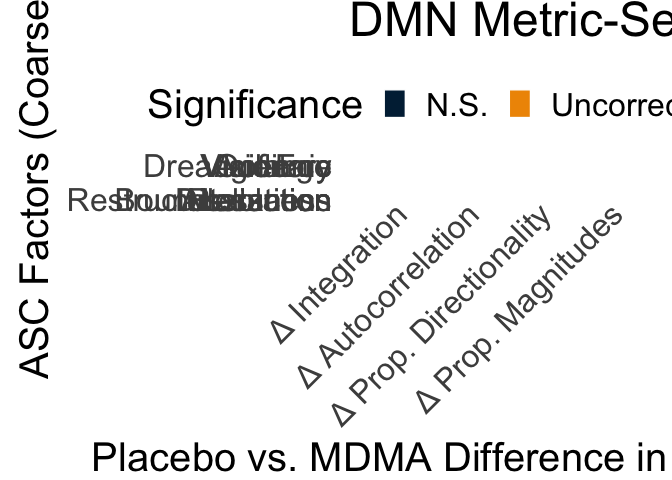
\includegraphics{Stats_n_Viz_files/figure-latex/unnamed-chunk-21-1.pdf}

\begin{Shaded}
\begin{Highlighting}[]
\CommentTok{\# DMN AUTOCOR}
\CommentTok{\# Create a dataframe with the values and column names}
\NormalTok{df }\OtherTok{\textless{}{-}} \FunctionTok{data.frame}\NormalTok{(}\AttributeTok{Values =}\NormalTok{ TA\_corvec, }\AttributeTok{pvals=}\NormalTok{TA\_pvec)}

\CommentTok{\# make a color vector by significance}
\NormalTok{colorvec}\OtherTok{=}\FunctionTok{rep}\NormalTok{(}\StringTok{\textquotesingle{}NS\textquotesingle{}}\NormalTok{,}\DecValTok{11}\NormalTok{)}
\NormalTok{colorvec[TA\_pvec}\SpecialCharTok{\textless{}}\NormalTok{.}\DecValTok{05}\NormalTok{]}\OtherTok{=}\StringTok{\textquotesingle{}Uncr\textquotesingle{}}
\NormalTok{colorvec[TA\_pvec\_mc}\SpecialCharTok{\textless{}}\NormalTok{.}\DecValTok{05}\NormalTok{]}\OtherTok{=}\StringTok{\textquotesingle{}FDR\textquotesingle{}}
\NormalTok{df}\SpecialCharTok{$}\NormalTok{Sig }\OtherTok{\textless{}{-}} \FunctionTok{factor}\NormalTok{(colorvec, }\AttributeTok{levels =} \FunctionTok{c}\NormalTok{(}\StringTok{\textquotesingle{}NS\textquotesingle{}}\NormalTok{, }\StringTok{\textquotesingle{}Uncr\textquotesingle{}}\NormalTok{, }\StringTok{\textquotesingle{}FDR\textquotesingle{}}\NormalTok{))}
\CommentTok{\# Specify color scale manually}
\NormalTok{colors }\OtherTok{\textless{}{-}} \FunctionTok{c}\NormalTok{(}\StringTok{\textquotesingle{}NS\textquotesingle{}} \OtherTok{=} \StringTok{\textquotesingle{}\#002642\textquotesingle{}}\NormalTok{, }\StringTok{\textquotesingle{}Uncr\textquotesingle{}} \OtherTok{=} \StringTok{\textquotesingle{}\#EF9500\textquotesingle{}}\NormalTok{, }\StringTok{\textquotesingle{}FDR\textquotesingle{}} \OtherTok{=} \StringTok{\textquotesingle{}\#840032\textquotesingle{}}\NormalTok{)}
\CommentTok{\# extra step needs to be done to maintain same row ordering as previous plot}
\NormalTok{df}\SpecialCharTok{$}\NormalTok{ColumnNamesAcr}\OtherTok{\textless{}{-}}\FunctionTok{c}\NormalTok{(dascNamesAcr)}
\NormalTok{df}\SpecialCharTok{$}\NormalTok{ColumnNamesAcr}\OtherTok{\textless{}{-}}\FunctionTok{factor}\NormalTok{(df}\SpecialCharTok{$}\NormalTok{ColumnNamesAcr,}\AttributeTok{levels=}\FunctionTok{c}\NormalTok{(}\StringTok{\textquotesingle{}Anx.\textquotesingle{}}\NormalTok{,}\StringTok{\textquotesingle{}B.S.\textquotesingle{}}\NormalTok{,}\StringTok{\textquotesingle{}C.M.O.P.\textquotesingle{}}\NormalTok{,}\StringTok{\textquotesingle{}C.Im.\textquotesingle{}}\NormalTok{,}\StringTok{\textquotesingle{}Disemb.\textquotesingle{}}\NormalTok{,}\StringTok{\textquotesingle{}E.Im.\textquotesingle{}}\NormalTok{,}\StringTok{\textquotesingle{}E.U.\textquotesingle{}}\NormalTok{,}\StringTok{\textquotesingle{}I.C.\textquotesingle{}}\NormalTok{,}\StringTok{\textquotesingle{}Ins.\textquotesingle{}}\NormalTok{,}\StringTok{\textquotesingle{}S.E.\textquotesingle{}}\NormalTok{,}\StringTok{\textquotesingle{}Syn.\textquotesingle{}}\NormalTok{))}
\CommentTok{\# bar version}
\FunctionTok{ggplot}\NormalTok{(df, }\FunctionTok{aes}\NormalTok{(}\AttributeTok{x =}\NormalTok{ Values, }\AttributeTok{y =}\NormalTok{ ColumnNamesAcr,}\AttributeTok{fill=}\NormalTok{Sig)) }\SpecialCharTok{+}
  \FunctionTok{geom\_bar}\NormalTok{(}\AttributeTok{size=}\DecValTok{3}\NormalTok{,}\AttributeTok{stat =} \StringTok{"identity"}\NormalTok{)}\SpecialCharTok{+}
  \FunctionTok{scale\_fill\_manual}\NormalTok{(}\AttributeTok{values =}\NormalTok{ colors) }\SpecialCharTok{+}
  \FunctionTok{labs}\NormalTok{(}\AttributeTok{y =} \StringTok{""}\NormalTok{, }\AttributeTok{x =} \StringTok{"Subscale Correlation"}\NormalTok{,}\AttributeTok{title=}\StringTok{"Change in Autocorrelation"}\NormalTok{)}\SpecialCharTok{+}\FunctionTok{theme\_minimal}\NormalTok{(}\AttributeTok{base\_size=}\DecValTok{17}\NormalTok{)}\SpecialCharTok{+}\FunctionTok{xlim}\NormalTok{(}\FunctionTok{c}\NormalTok{(}\SpecialCharTok{{-}}\NormalTok{.}\DecValTok{3}\NormalTok{,.}\DecValTok{8}\NormalTok{))}\SpecialCharTok{+}
  \FunctionTok{theme}\NormalTok{(}\AttributeTok{legend.position=}\StringTok{\textquotesingle{}none\textquotesingle{}}\NormalTok{)}
\end{Highlighting}
\end{Shaded}

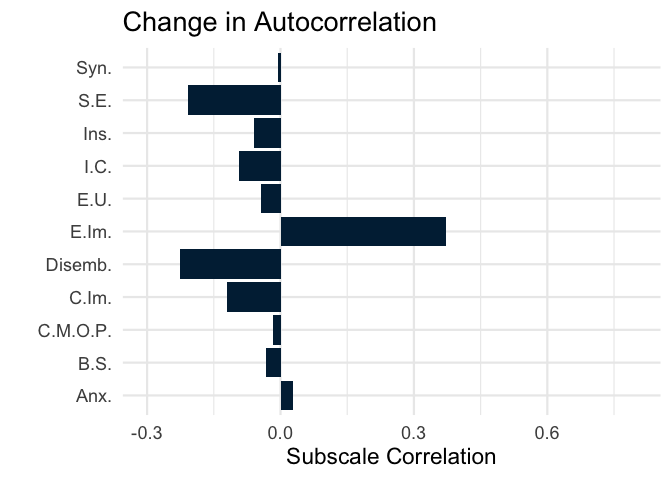
\includegraphics{Stats_n_Viz_files/figure-latex/unnamed-chunk-21-2.pdf}

\begin{Shaded}
\begin{Highlighting}[]
\CommentTok{\# DMN BUP}
\CommentTok{\# Create a dataframe with the values and column names}
\NormalTok{df }\OtherTok{\textless{}{-}} \FunctionTok{data.frame}\NormalTok{(}\AttributeTok{Values =}\NormalTok{ BUP\_corvec, }\AttributeTok{pvals=}\NormalTok{BUP\_pvec)}

\CommentTok{\# make a color vector by significance}
\NormalTok{colorvec}\OtherTok{=}\FunctionTok{rep}\NormalTok{(}\StringTok{\textquotesingle{}NS\textquotesingle{}}\NormalTok{,}\DecValTok{11}\NormalTok{)}
\NormalTok{colorvec[BUP\_pvec}\SpecialCharTok{\textless{}}\NormalTok{.}\DecValTok{05}\NormalTok{]}\OtherTok{=}\StringTok{\textquotesingle{}Uncr\textquotesingle{}}
\NormalTok{colorvec[BUP\_pvec\_mc}\SpecialCharTok{\textless{}}\NormalTok{.}\DecValTok{05}\NormalTok{]}\OtherTok{=}\StringTok{\textquotesingle{}FDR\textquotesingle{}}
\NormalTok{df}\SpecialCharTok{$}\NormalTok{Sig }\OtherTok{\textless{}{-}} \FunctionTok{factor}\NormalTok{(colorvec, }\AttributeTok{levels =} \FunctionTok{c}\NormalTok{(}\StringTok{\textquotesingle{}NS\textquotesingle{}}\NormalTok{, }\StringTok{\textquotesingle{}Uncr\textquotesingle{}}\NormalTok{, }\StringTok{\textquotesingle{}FDR\textquotesingle{}}\NormalTok{))}
\CommentTok{\# Specify color scale manually}
\NormalTok{colors }\OtherTok{\textless{}{-}} \FunctionTok{c}\NormalTok{(}\StringTok{\textquotesingle{}NS\textquotesingle{}} \OtherTok{=} \StringTok{\textquotesingle{}\#002642\textquotesingle{}}\NormalTok{, }\StringTok{\textquotesingle{}Uncr\textquotesingle{}} \OtherTok{=} \StringTok{\textquotesingle{}\#EF9500\textquotesingle{}}\NormalTok{, }\StringTok{\textquotesingle{}FDR\textquotesingle{}} \OtherTok{=} \StringTok{\textquotesingle{}\#840032\textquotesingle{}}\NormalTok{)}
\CommentTok{\# extra step needs to be done to maintain same row ordering as previous plot}
\NormalTok{df}\SpecialCharTok{$}\NormalTok{ColumnNamesAcr}\OtherTok{\textless{}{-}}\FunctionTok{c}\NormalTok{(dascNamesAcr)}
\NormalTok{df}\SpecialCharTok{$}\NormalTok{ColumnNamesAcr}\OtherTok{\textless{}{-}}\FunctionTok{factor}\NormalTok{(df}\SpecialCharTok{$}\NormalTok{ColumnNamesAcr,}\AttributeTok{levels=}\FunctionTok{c}\NormalTok{(}\StringTok{\textquotesingle{}Anx.\textquotesingle{}}\NormalTok{,}\StringTok{\textquotesingle{}B.S.\textquotesingle{}}\NormalTok{,}\StringTok{\textquotesingle{}C.M.O.P.\textquotesingle{}}\NormalTok{,}\StringTok{\textquotesingle{}C.Im.\textquotesingle{}}\NormalTok{,}\StringTok{\textquotesingle{}Disemb.\textquotesingle{}}\NormalTok{,}\StringTok{\textquotesingle{}E.Im.\textquotesingle{}}\NormalTok{,}\StringTok{\textquotesingle{}E.U.\textquotesingle{}}\NormalTok{,}\StringTok{\textquotesingle{}I.C.\textquotesingle{}}\NormalTok{,}\StringTok{\textquotesingle{}Ins.\textquotesingle{}}\NormalTok{,}\StringTok{\textquotesingle{}S.E.\textquotesingle{}}\NormalTok{,}\StringTok{\textquotesingle{}Syn.\textquotesingle{}}\NormalTok{))}

\CommentTok{\# bar version}
\FunctionTok{ggplot}\NormalTok{(df, }\FunctionTok{aes}\NormalTok{(}\AttributeTok{x =}\NormalTok{ Values, }\AttributeTok{y =}\NormalTok{ ColumnNamesAcr,}\AttributeTok{fill=}\NormalTok{Sig)) }\SpecialCharTok{+}
  \FunctionTok{geom\_bar}\NormalTok{(}\AttributeTok{size=}\DecValTok{3}\NormalTok{,}\AttributeTok{stat =} \StringTok{"identity"}\NormalTok{)}\SpecialCharTok{+}
  \FunctionTok{scale\_fill\_manual}\NormalTok{(}\AttributeTok{values =}\NormalTok{ colors) }\SpecialCharTok{+}
  \FunctionTok{labs}\NormalTok{(}\AttributeTok{y =} \StringTok{""}\NormalTok{, }\AttributeTok{x =} \StringTok{"Subscale Correlation"}\NormalTok{,}\AttributeTok{title=}\StringTok{"Change in Prop. Direction"}\NormalTok{)}\SpecialCharTok{+}\FunctionTok{theme\_minimal}\NormalTok{(}\AttributeTok{base\_size=}\DecValTok{17}\NormalTok{)}\SpecialCharTok{+}\FunctionTok{xlim}\NormalTok{(}\FunctionTok{c}\NormalTok{(}\SpecialCharTok{{-}}\NormalTok{.}\DecValTok{3}\NormalTok{,.}\DecValTok{8}\NormalTok{))}\SpecialCharTok{+}
  \FunctionTok{theme}\NormalTok{(}\AttributeTok{legend.position=}\StringTok{\textquotesingle{}none\textquotesingle{}}\NormalTok{)}
\end{Highlighting}
\end{Shaded}

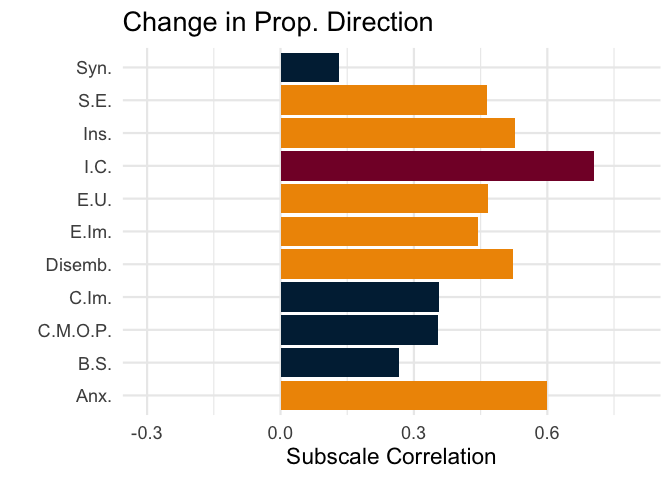
\includegraphics{Stats_n_Viz_files/figure-latex/unnamed-chunk-21-3.pdf}

\begin{Shaded}
\begin{Highlighting}[]
\CommentTok{\# and one just for the legend}
\NormalTok{df}\SpecialCharTok{$}\NormalTok{Significant}\OtherTok{=}\NormalTok{df}\SpecialCharTok{$}\NormalTok{Sig}
\FunctionTok{ggplot}\NormalTok{(df, }\FunctionTok{aes}\NormalTok{(}\AttributeTok{x =}\NormalTok{ Values, }\AttributeTok{y =}\NormalTok{ ColumnNamesAcr,}\AttributeTok{fill=}\NormalTok{Significant)) }\SpecialCharTok{+}
  \FunctionTok{geom\_bar}\NormalTok{(}\AttributeTok{size=}\DecValTok{3}\NormalTok{,}\AttributeTok{stat =} \StringTok{"identity"}\NormalTok{)}\SpecialCharTok{+}
  \FunctionTok{scale\_fill\_manual}\NormalTok{(}\AttributeTok{values =}\NormalTok{ colors) }\SpecialCharTok{+}
  \FunctionTok{labs}\NormalTok{(}\AttributeTok{y =} \StringTok{""}\NormalTok{, }\AttributeTok{x =} \StringTok{"Subscale Correlation"}\NormalTok{,}\AttributeTok{title=}\StringTok{"Change in Prop. Direction"}\NormalTok{)}\SpecialCharTok{+}\FunctionTok{theme\_minimal}\NormalTok{(}\AttributeTok{base\_size=}\DecValTok{17}\NormalTok{)}\SpecialCharTok{+}\FunctionTok{xlim}\NormalTok{(}\FunctionTok{c}\NormalTok{(}\SpecialCharTok{{-}}\NormalTok{.}\DecValTok{3}\NormalTok{,.}\DecValTok{8}\NormalTok{))}
\end{Highlighting}
\end{Shaded}

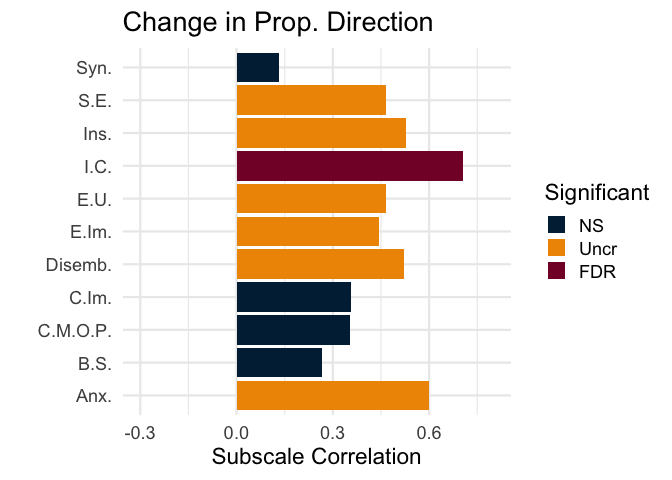
\includegraphics{Stats_n_Viz_files/figure-latex/unnamed-chunk-21-4.pdf}

\begin{Shaded}
\begin{Highlighting}[]
\CommentTok{\# DMN Mag}
\CommentTok{\# Create a dataframe with the values and column names}
\NormalTok{df }\OtherTok{\textless{}{-}} \FunctionTok{data.frame}\NormalTok{(}\AttributeTok{Values =}\NormalTok{ M\_corvec, }\AttributeTok{pvals=}\NormalTok{M\_pvec)}

\CommentTok{\# make a color vector by significance}
\NormalTok{colorvec}\OtherTok{=}\FunctionTok{rep}\NormalTok{(}\StringTok{\textquotesingle{}NS\textquotesingle{}}\NormalTok{,}\DecValTok{11}\NormalTok{)}
\NormalTok{colorvec[M\_pvec}\SpecialCharTok{\textless{}}\NormalTok{.}\DecValTok{05}\NormalTok{]}\OtherTok{=}\StringTok{\textquotesingle{}Uncr\textquotesingle{}}
\NormalTok{colorvec[M\_pvec\_mc}\SpecialCharTok{\textless{}}\NormalTok{.}\DecValTok{05}\NormalTok{]}\OtherTok{=}\StringTok{\textquotesingle{}FDR\textquotesingle{}}
\NormalTok{df}\SpecialCharTok{$}\NormalTok{Sig }\OtherTok{\textless{}{-}} \FunctionTok{factor}\NormalTok{(colorvec, }\AttributeTok{levels =} \FunctionTok{c}\NormalTok{(}\StringTok{\textquotesingle{}NS\textquotesingle{}}\NormalTok{, }\StringTok{\textquotesingle{}Uncr\textquotesingle{}}\NormalTok{, }\StringTok{\textquotesingle{}FDR\textquotesingle{}}\NormalTok{))}
\CommentTok{\# Specify color scale manually}
\NormalTok{colors }\OtherTok{\textless{}{-}} \FunctionTok{c}\NormalTok{(}\StringTok{\textquotesingle{}NS\textquotesingle{}} \OtherTok{=} \StringTok{\textquotesingle{}\#002642\textquotesingle{}}\NormalTok{, }\StringTok{\textquotesingle{}Uncr\textquotesingle{}} \OtherTok{=} \StringTok{\textquotesingle{}\#EF9500\textquotesingle{}}\NormalTok{, }\StringTok{\textquotesingle{}FDR\textquotesingle{}} \OtherTok{=} \StringTok{\textquotesingle{}\#840032\textquotesingle{}}\NormalTok{)}
\NormalTok{df}\SpecialCharTok{$}\NormalTok{ColumnNamesAcr}\OtherTok{\textless{}{-}}\FunctionTok{c}\NormalTok{(dascNamesAcr)}
\CommentTok{\# bar version}
\FunctionTok{ggplot}\NormalTok{(df, }\FunctionTok{aes}\NormalTok{(}\AttributeTok{x =}\NormalTok{ Values, }\AttributeTok{y =}\NormalTok{ ColumnNamesAcr,}\AttributeTok{fill=}\NormalTok{Sig)) }\SpecialCharTok{+}
  \FunctionTok{geom\_bar}\NormalTok{(}\AttributeTok{size=}\DecValTok{3}\NormalTok{,}\AttributeTok{stat =} \StringTok{"identity"}\NormalTok{)}\SpecialCharTok{+}
  \FunctionTok{scale\_fill\_manual}\NormalTok{(}\AttributeTok{values =}\NormalTok{ colors) }\SpecialCharTok{+}
  \FunctionTok{labs}\NormalTok{(}\AttributeTok{y =} \StringTok{""}\NormalTok{, }\AttributeTok{x =} \StringTok{"Subscale Correlation"}\NormalTok{,}\AttributeTok{title=}\StringTok{"Change in Prop. Magnitudes"}\NormalTok{)}\SpecialCharTok{+}\FunctionTok{theme\_minimal}\NormalTok{(}\AttributeTok{base\_size=}\DecValTok{17}\NormalTok{)}\SpecialCharTok{+}\FunctionTok{xlim}\NormalTok{(}\FunctionTok{c}\NormalTok{(}\SpecialCharTok{{-}}\NormalTok{.}\DecValTok{3}\NormalTok{,.}\DecValTok{8}\NormalTok{))}\SpecialCharTok{+}
  \FunctionTok{theme}\NormalTok{(}\AttributeTok{legend.position=}\StringTok{\textquotesingle{}none\textquotesingle{}}\NormalTok{)}
\end{Highlighting}
\end{Shaded}

\begin{verbatim}
## Warning: Removed 1 row containing missing values or values outside the scale range
## (`geom_bar()`).
\end{verbatim}

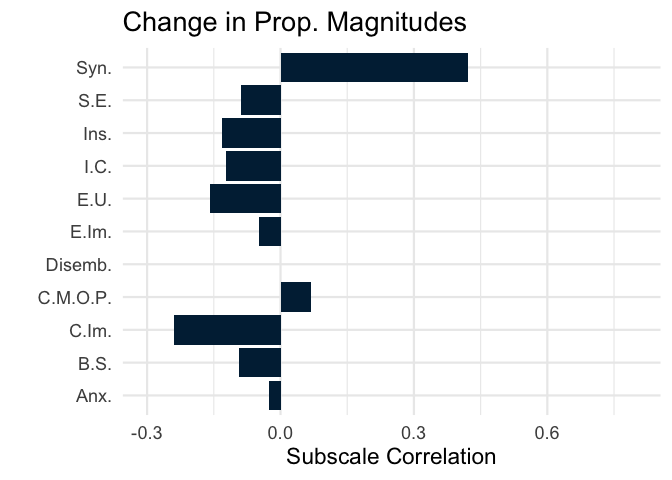
\includegraphics{Stats_n_Viz_files/figure-latex/unnamed-chunk-21-5.pdf}

\begin{Shaded}
\begin{Highlighting}[]
\CommentTok{\# pull out BUP\textasciitilde{}Impaired Control correlation}
\FunctionTok{ggplot}\NormalTok{(}\AttributeTok{data=}\NormalTok{DAS\_changeDF\_people,}\FunctionTok{aes}\NormalTok{(}\AttributeTok{y=}\NormalTok{dascscore\_impair,}\AttributeTok{x=}\NormalTok{BUP\_Decrease))}\SpecialCharTok{+}
  \FunctionTok{geom\_point}\NormalTok{(}\AttributeTok{size=}\DecValTok{4}\NormalTok{,}\FunctionTok{aes}\NormalTok{(}\AttributeTok{color =}\NormalTok{ People))}\SpecialCharTok{+}
  \FunctionTok{labs}\NormalTok{(}\AttributeTok{x =} \StringTok{"Decrease in Bottom{-}up \%"}\NormalTok{, }\AttributeTok{y =} \StringTok{"Increase in Impaired Control"}\NormalTok{, }\AttributeTok{color =} \StringTok{"People"}\NormalTok{) }\SpecialCharTok{+}
  \FunctionTok{scale\_color\_manual}\NormalTok{(}\AttributeTok{values =}\NormalTok{ generated\_colors) }\SpecialCharTok{+}
  \FunctionTok{theme\_minimal}\NormalTok{(}\AttributeTok{base\_size =} \DecValTok{16}\NormalTok{)}
\end{Highlighting}
\end{Shaded}

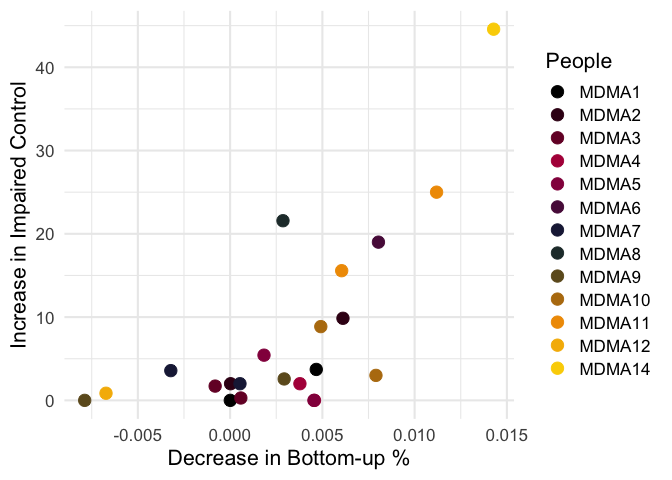
\includegraphics{Stats_n_Viz_files/figure-latex/unnamed-chunk-21-6.pdf}

\begin{Shaded}
\begin{Highlighting}[]
\FunctionTok{cor.test}\NormalTok{(DAS\_changeDF\_people}\SpecialCharTok{$}\NormalTok{dascscore\_impair,DAS\_changeDF\_people}\SpecialCharTok{$}\NormalTok{BUP\_Decrease)}
\end{Highlighting}
\end{Shaded}

\begin{verbatim}
## 
##  Pearson's product-moment correlation
## 
## data:  DAS_changeDF_people$dascscore_impair and DAS_changeDF_people$BUP_Decrease
## t = 4.4524, df = 20, p-value = 0.0002444
## alternative hypothesis: true correlation is not equal to 0
## 95 percent confidence interval:
##  0.4041507 0.8687335
## sample estimates:
##       cor 
## 0.7055399
\end{verbatim}

\end{document}
